\chapter{Chaîne de Simulation}
\label{chapter4}

\section{Motivations}

Afin de pouvoir r\'ealiser des \'etudes d'alignement d'\'echelles double face \textit{PLUME} et de super-plans \textit{SALAT}, une simulation num\'erique de ces objets est requise. C'est pourquoi, une cha\^ine de simulation capable de reproduire les caract\'eristiques des capteurs CMOS d\'evelopp\'es au sein de l'IPHC a \'et\'e mise en place. Cette simulation permettra d'étudier \`a la fois les capteurs de grande surface \'equipant le t\'elescope \textit{SALAT} mais aussi les \'echelles double face de type \textit{PLUME}. Nous d\'ecrirons premi\`erement le fonctionnement de la simulation d'un capteur CMOS bas\'ee sur le logiciel \textit{GEANT4} et sur les capteurs \textit{MIMOSA-22 AHR} et \textit{MIMOSA-28 HR15}. Pour cela nous \'etudierons le d\'ep\^ot de charges dans la couche épitaxiée du capteur simul\'e puis nous effectuerons le transport de ces charges vers les pixels. Ensuite nous ajusterons les param\`etres de la simulation afin de reproduire les performances des capteurs r\'eels. Enfin, nous \'etudierons les performances de quelques t\'elescopes simul\'es.

\section{Description et fonctionnement}

  Dans cette partie nous pr\'esenterons la conception d'une chaîne de simulation compl\`ete de capteurs CMOS. Elle se base sur le logiciel GEANT4 et sur l'\'etude des capteurs analogiques effectu\'ee par le groupe. Ce travail a \'et\'e initi\'e afin de posséder une simulation Monte-Carlo rendant compte des propri\'et\'es des capteurs d\'evelopp\'es dans le groupe.

  \subsection{MIMOSA-22 AHR et MIMOSA-28 THR}
  
  Les capteurs MIMOSA-22 AHR et MIMOSA-28 HR15 sont les deux capteurs \`a la base de notre simulation. La matrice S7 de MIMOSA-22 AHR est \`a sortie analogique alors que le capteur MIMOSA-28 HR15, bas\'e sur la matrice S7 de MIMOSA-22 AHR est un capteur \`a sortie digitale incluant une suppression de z\'eros. Une sortie analogique beaucoup plus lente, r\'eserv\'ee aux tests en laboratoire, est aussi pr\'esente sur MIMOSA-28 HR15. Les tests en faisceau du capteur MIMOSA-22 AHR nous permettront plus loin de conna\^itre la r\'epartition des charges collect\'es dans les pixels des amas. Ces deux capteurs sont r\'ealis\'es avec la technologie AMS dot\'ee d'une taille de grille de 0.35 $\mu m$. Ce processus de fabrication permet d'introduire une couche \'epitaxi\'ee de haute r\'esistivit\'e ($> 400 \, \Omega.cm$). Cette haute r\'esistivit\'e permet d'augmenter la zone d\'epl\'et\'ee autour des diodes N-Well.
 
   \begin{figure}[!htb]
   \begin{center}
    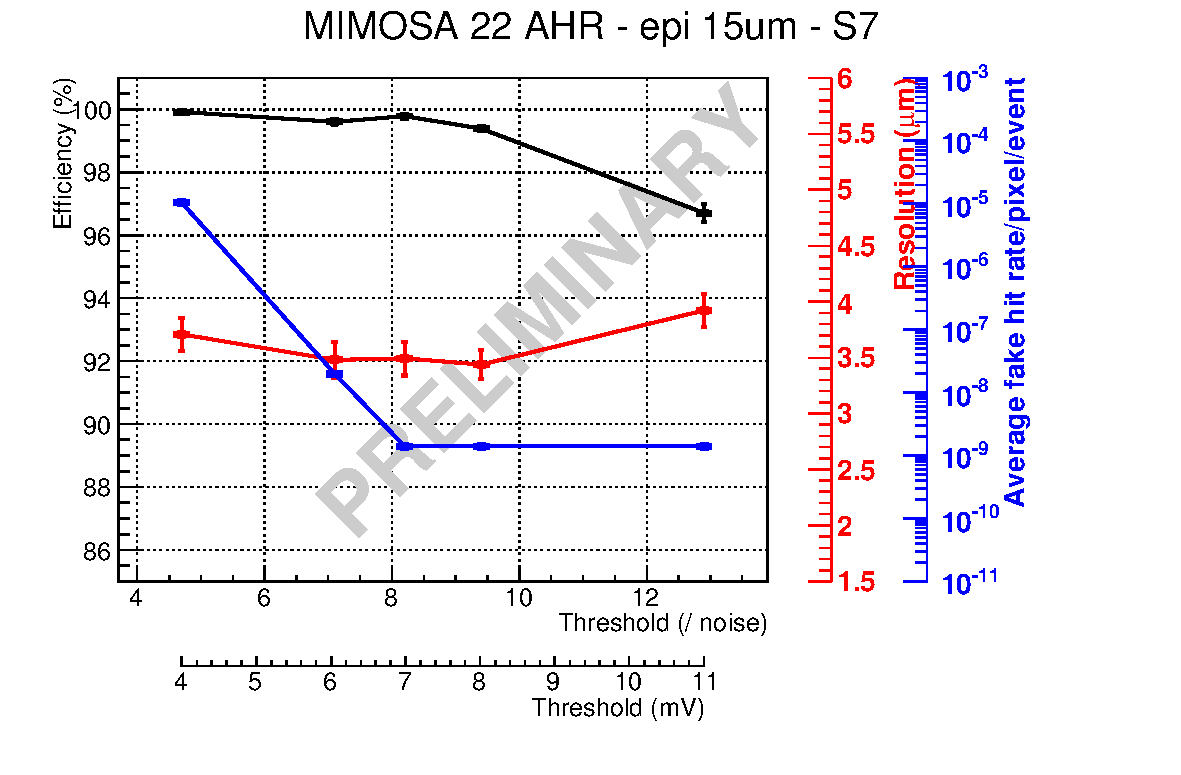
\includegraphics[scale=0.60]{./figures/perf_MI22AHR-S7-eps-converted-to.pdf}
    \caption{Performances de la matrice S7 du capteur MIMOSA-22 AHR. En noir l'efficacit\'e de d\'etection, en bleu le taux d'impacts fant\^omes et en rouge la r\'esolution spatiale en fonction du seuil des discriminateurs en multiple du bruit moyen ou en $mV$.}
    \label{fig:Mi22AHR}
   \end{center}
  \end{figure}
  
   La campagne de tests de MIMOSA-22 AHR a \'et\'e effectu\'ee au SPS avec un faisceau de pions charg\'es d'impulsion 120 $GeV/c$. Durant les prises de donn\'ees, un refroidissement \`a 20 \ensuremath{^\circ C} du \textit{DUT} a \'et\'e r\'ealis\'e. Les performances de la matrice de pixels S7 du capteur MIMOSA-22 AHR sont illustr\'ees en figure \ref{fig:Mi22AHR}. Au seuil de $7 \, \sigma$ cette matrice fournit une efficacit\'e sup\'erieure \`a 99 $\%$ pour un taux de fant\^omes inférieurs \`a $10^{-6}$ et une r\'esolution spatiale d'environ 3.5 $\mu m$.
 
  \medskip
 
  \begin{figure}[!htb]
   \begin{center} 
    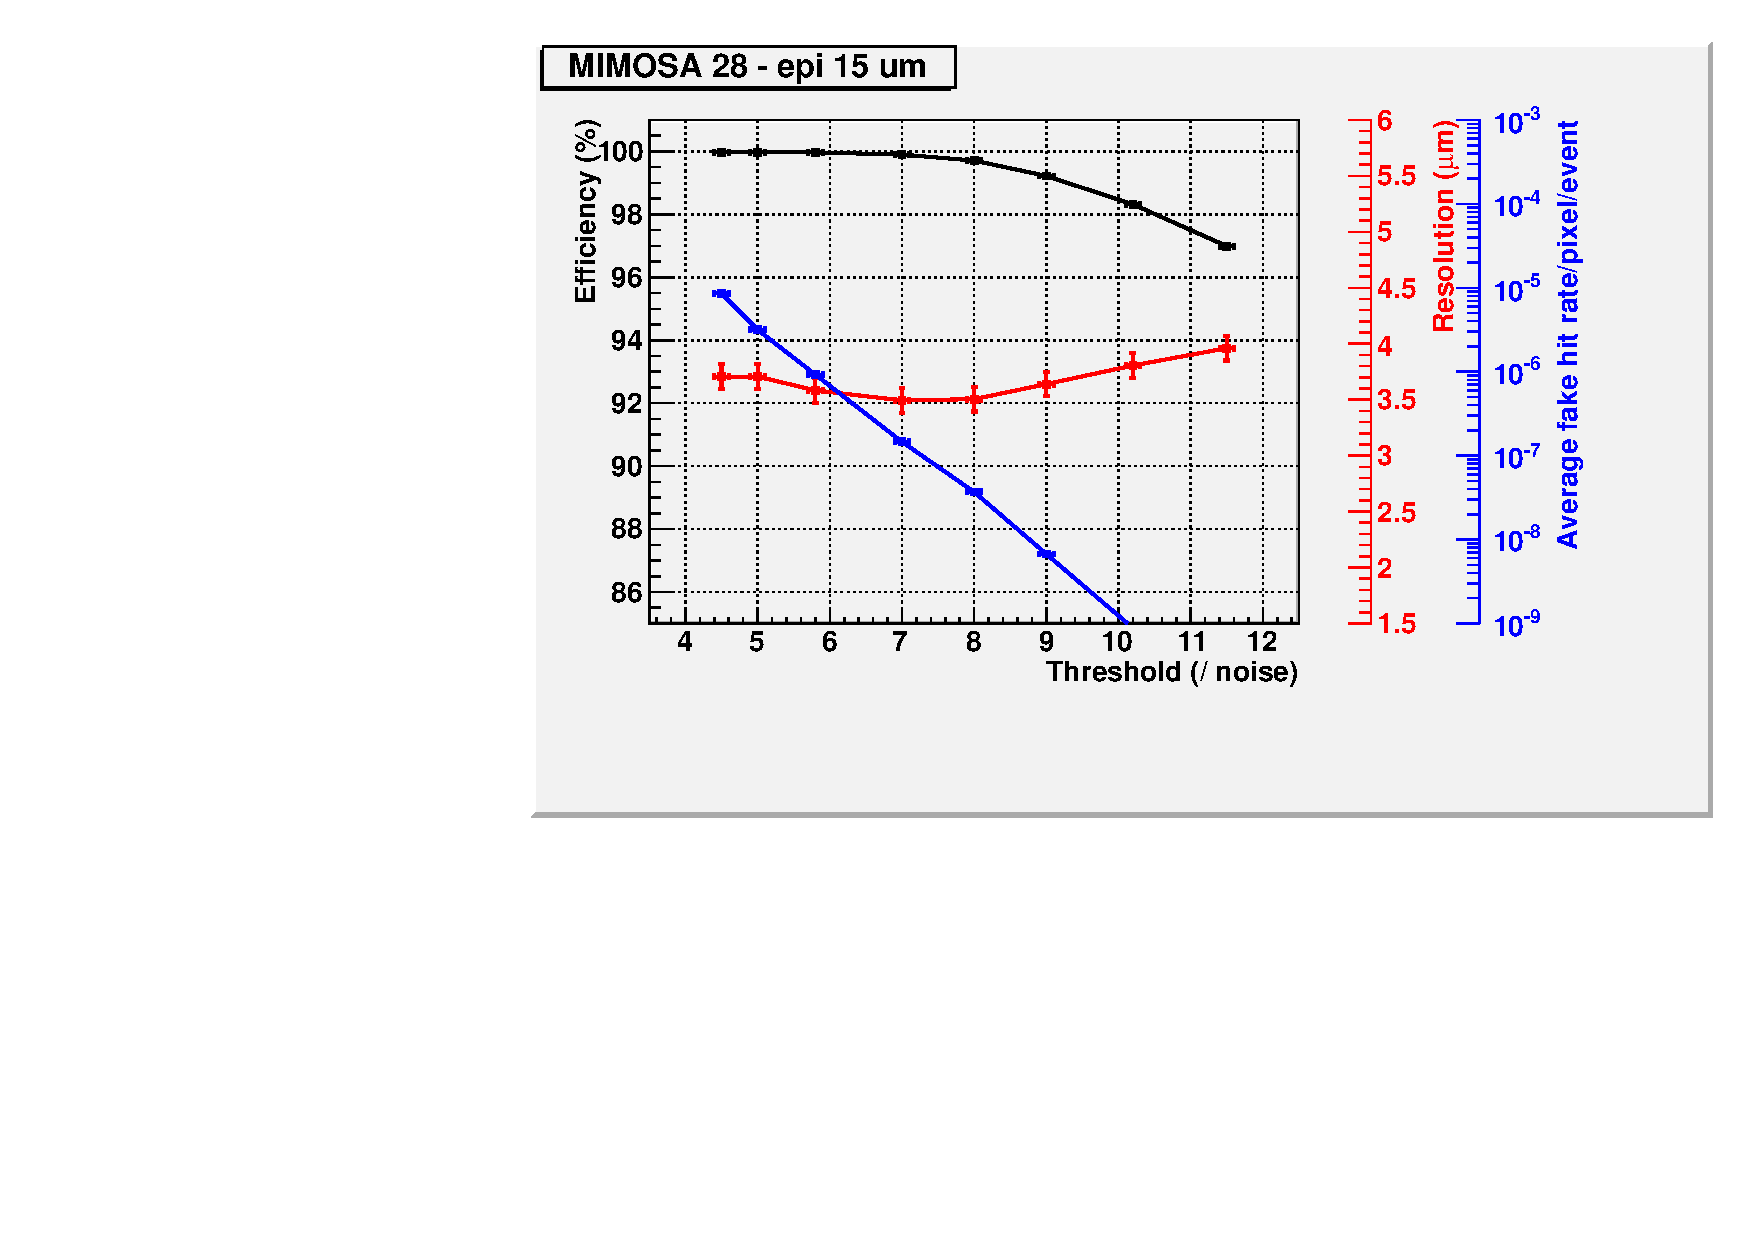
\includegraphics[scale=0.60]{./figures/Mi28_results.pdf}
    \caption{Performances du capteur MIMOSA28 HR15. En noir l'efficacit\'e de d\'etection, en bleu le taux d'impacts fant\^omes et en rouge la r\'esolution spatiale. Les tests ont \'et\'e effectu\'es avec une temp\'erature de 15 \ensuremath{^\circ C} }
    \label{fig:Mim28perf}
   \end{center}
  \end{figure} 

  Nous allons \`a pr\'esent dresser le portrait des caract\'eristiques du capteur MIMOSA-28 HR15. Comme son nom l'indique, il poss\`ede une couche épitaxiée de haute r\'esistivit\'e d'environ 15 $\mu m$ d'\'epaisseur. Ce capteur a \'et\'e \'etudi\'e durant la campagne de test en faisceau d'octobre 2011 au SPS avec un faisceau de pions charg\'es dot\'es d'une impulsion de 120 $GeV/c$. Nous allons nous atteler \`a \'etudier les param\`etres cl\'es qui caract\'erisent ce capteur CMOS, \`a savoir, l'efficacit\'e de d\'etection, le taux d'impacts fant\^omes et la r\'esolution spatiale. La figure \ref{fig:Mim28perf} r\'esume les performances obtenues. L'efficacit\'e de d\'etection et le taux d'impacts fant\^omes sont deux param\`etres li\'es qui d\'ependent du seuil appliqu\'e au capteur. Un balayage en seuil a \'et\'e effectu\'e pour des seuils appliqu\'es aux discriminateurs allant de 4 \`a 11.5 fois la valeur moyenne du bruit. Le but de cette op\'eration est de trouver un point de fonctionnement alliant l'efficacit\'e la plus \'elev\'ee possible avec un taux d'impacts fant\^omes acceptable. Plus le seuil est \'elev\'e plus l'efficacit\'e et le taux d'impacts fant\^omes diminuent. La r\'esolution spatiale varie quant \`a elle entre 3.5 et 4 $\mu m$ avec son minimum de 3.5 $\mu m$ atteint pour les seuils de 7 et 8 $\sigma$. Le point de fonctionnement choisi est celui pour un seuil des discriminateurs de 7 $\sigma$. L'efficacit\'e est alors de $99.9 \, \%$ pour un taux d'impacts fant\^omes de $1.6 \, 10^{-7}$ et une r\'esolution de 3.5 $\mu m$.
  
%  Haute resistivit\'e
%  Description mimosa 22 thra
%  Descritpion mimosa 28 thr
  
  
  \subsection{Simulation de capteurs CMOS avec GEANT4}

    \subsubsection{GEANT4}
    
%Le framework Geant4 est composé de différents paquetages, qui permettent de définir tous les aspects de la simulation :
%Géometrie spécifie la disposition et les propriétés physiques de tous les éléments présents (détecteurs, absorbeurs, etc...).
%Tracking simule le passage des particules à travers la matière. Il prend en compte les interactions et les processus de désintégration radioactive possibles.
%Détection enregistre une particule quand elle entre dans le volume lié au détecteur et simule la réponse effective du détecteur.
%Run management enregistre les détails de chaque run, où un run est une collection d'évènements tout simulés dans des conditions identiques. Ce module permet de gérer le changement des conditions expérimentales d'un run à l'autre.
%Visualisation: Geant4 offre plusieurs options, notamment OpenGL, pour visualiser la géométrie d'une expérience et les trajectoires simulées.
%Une interface utilisateur basée sur tcsh est disponible, qui permet de commander la simulation soit interactivement soit par un script.
   
    Pour nos simulations Monte Carlo, nous allons utiliser le logiciel \textit{GEANT4}. \textit{GEANT4} est une plate-forme logicielle disponible dans le domaine public, et téléchargeable gratuitement, permettant de r\'ealiser des simulations Monte-Carlo de particules traversant la mati\`ere. Bas\'ee sur le langage C++ et la programmation orient\'ee objet on compte parmi ses fonctionnalit\'es : la construction d'une géométrie, différents mod\`eles de physique, une gestion des impacts, un syst\`eme de trajectom\'etrie et un syst\`eme de visualisation. 
    
%     La figure ~\ref{fig:graphG4} illustre ces fonctionnalit\'es.
    
%     \begin{figure}[h]
%     \begin{center}
%     \begin{tikzpicture}
%      \path[small mindmap,concept color=black,text=white]
%        node[concept] {\textbf{GEANT4}}
%        [clockwise from=0]
%        child[concept color=green!50!black] {
%        node[concept] {\textbf{G\'eom\'etrie : G4Detector Construction}}
%        [clockwise from=45]
%        child { node[concept] {\textbf{G\'eom\'etrie de l'exp\'erience}} }
%        child { node[concept] {\textbf{Mat\'eriaux, densit\'e, ...}} }
%        }  
%        child[concept color=blue] {
%        node[concept] {\textbf{Faisceau : G4Primary Event Action}}
%        [clockwise from=-30]
%        child { node[concept] {\textbf{Type de particule}} }
%        child { node[concept] {\textbf{Position initiale et direction}} }
%        child { node[concept] {\textbf{Impulsion}} }
%        }
%        child[concept color=red] {
%        node[concept] {\textbf{Mod\`eles de physique : G4Physic List}} 
%        [clockwise from=-120]
%        child { node[concept] {\textbf{Type de particules}} }
%        child { node[concept] {\textbf{Processus d'interactions}} }
%        }
%        child[concept color=purple] { 
%        node[concept] {\textbf{Gestion des impacts}} 
%        [clockwise from=-150]
%        child { node[concept] {\textbf{Gestion des coups}} }
%        child { node[concept] {\textbf{Gestion des coups digitis\'es}} }
%        }
%        child[concept color=orange] { node[concept] {\textbf{Visuali- sation}} };
%     \end{tikzpicture}
%     \end{center}
%     \caption{Graphe des principales fonctionnalit\'es de GEANT4.}
%     \label{fig:graphG4}
%     \end{figure}
%     
    \paragraph{Principe de base}

    \textit{GEANT4} est bas\'e sur le principe de la simulation Monte-Carlo. Il s'agit d'une m\'ethode ayant pour objectif le calcul de valeurs num\'eriques \`a l'aide de proc\'ed\'es probabilistes d\'ecrivant les processus physiques \'etudi\'es. Dans \textit{GEANT4} le transport des particules \`a travers la mati\`ere est d\'ecoup\'e en plusieurs \'el\'ements appel\'es \textit{pas} ou \textit{step}. \`A chaque \textit{step} la direction et la perte d'\'energie de la particule sont calcul\'ees. La particule peut aussi, par exemple, se d\'esint\'egrer en plusieurs autres particules ou être stopp\'ee par la mati\`ere. \\
    
%     Cette m\'ethode fut d\'ecrite pour la premi\`ere fois dans un article co-\'ecrit par Nicholas Metropolis et Stanislaw Ulam en 1949 \cite{Metropolis_et_Stanislaw} dans le cadre du projet Manatthan ayant pour but le développement de la bombe atomique aux \'Etats-unis. 
   
%     ou interagir selon un autre proc\'ed\'e physique.

    \paragraph{Mod\`eles de physique}
    
    Dans \textit{GEANT4}, il existe différents mod\`eles de lois physiques r\'egissant le comportement des particules. Ces lois, appel\'ees \textit{physics list} peuvent être choisies en fonction du type de physique mis en jeu dans l'exp\'erience. Par exemple, il existe des \textit{physics list} pour les interactions \'electromagn\'etiques ou hadroniques. Le choix de la \textit{physics list} est r\'ealis\'e en fonction du type de particule et du domaine en \'energie voulus. Dans notre simulation, les fichiers relatifs \`a la \textit{physics list} sont : \textit{DigiCmosPhysicsList.cc} et \textit{DigiCMOS.cc}. Dans notre cas on utilise la \textit{physics list} \textit{FTFP\_BERT}. En particulier, elle g\`ere les processus de \textit{bremsstrahlung}, d'ionisation, de diffusion multiple, de production de paires, d'annihilation et de d\'esint\'egrations.  \\
    
    \paragraph{Géométrie}
   
    Con\c{c}u pour construire différentes g\'eom\'etries des plus simples aux plus complexes, \textit{GEANT4} dispose de m\'ethodes ing\'enieuses pour r\'ealiser simplement la g\'eom\'etrie d\'esir\'ee. Dans \textit{GEANT4} la g\'eom\'etrie est construite \`a base de volumes. Il existe 2 types de volumes, les volumes physiques et les volumes logiques. 
    
    \medskip
    
    Les volumes logiques poss\`edent une forme pr\'ealablement définie et peuvent accueillir d'autres volumes logiques. Ils ont comme propri\'et\'e la nature du mat\'eriau qui le constitue et peuvent aussi être sensibles aux passages des particules qui le traversent. Lorsque un volume est sensible, il renvoie les coordonn\'ees des \textit{steps} qui le traversent dans le r\'ef\'erentiel de son volume logique et la quantit\'e d'\'energie d\'epos\'ee. Cependant, les volumes logiques ne contiennent pas d'information sur la localisation physique du volume dans le d\'etecteur. Le volume logique de base, c'est \`a dire celui qui contient toute l'exp\'erience est appel\'e \textit{World}.
    
    \medskip
    
    Les volumes dits physiques sont ceux qui contiennent les informations de positions des volumes logiques fils par rapport aux volumes logiques parents. Ainsi, un volume logique peut contenir un empilement d'autres volumes logiques, \`a la condition que ceux-ci ne se chevauchent pas. Un m\^eme volume logique, qui contient tous ses sous-volumes, peut \^etre r\'epliqu\'e \`a plusieurs endroits dans le d\'etecteur. Cela permet un gain non n\'egligeable de m\'emoire vive consomm\'ee.
    
    \medskip
    
    Chaque volume logique peut adopter une forme pr\'ed\'efinie. Le volume peut être cubique, cylindrique, sph\'erique, trap\'ezo\"idal, etc ... Si la forme voulue n'est pas pr\'esente dans les formes de base, on peut la cr\'eer par union, soustraction ou intersection de formes de base. Ainsi, une g\'eom\'etrie est constitu\'ee d'un empilement de volumes logiques plac\'es physiquement dans le volume \textit{World} grâce aux volumes physiques. Ils forment alors un empilement de blocs qui constituent l'expérience d\'esir\'ee. 
    
%     Dans notre simulation les fichiers relatifs aux g\'eom\'etries sont : \textit{DigiCmosDetectorConstruction.cc}, \textit{mimosaSensor.cc}, \textit{ladderSimpleFace.cc}, \textit{ladderPLUME.cc} et \textit{salat.cc}.
    
    \paragraph{Gestion des impacts}

    Comme vu pr\'ec\'edemment, certains volumes peuvent \^etre sensibles c'est-\`a-dire renvoyer les propri\'et\'es des \textit{step} qui le traverse. Un syst\`eme de collection d'impacts est impl\'ement\'e dans \textit{GEANT4}, il permet de stocker les diff\'erents impacts collect\'es par les volumes sensibles. A chaque volume sensible correspond une collection d'impacts diff\'erente. Pour chaque impact les positions des extr\'emités des \textit{step} appel\'ees \textit{pre-step} et \textit{post-step} (voir figure \ref{fig:step}), le temps de vol ainsi que l'\'energie d\'eposée le long des \textit{step} sont enregistr\'es. Dans notre simulation, les fichiers relatifs \`a ces collections sont \textit{DigiCmosChipSD.cc} et \textit{DigiCmosChipHit.cc}.
    
    \begin{figure}[!htb]
     \begin{center} 
      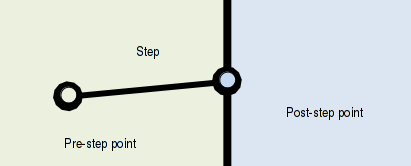
\includegraphics[scale=0.60]{./figures/step_geant4.png}
      \caption{\textit{Pre-step} et \textit{post-step} dans \textit{GEANT4}.}
      \label{fig:step}
     \end{center}
    \end{figure}
    
    Dans notre simulation, un autre syst\`eme de collections est utilis\'e, il s'agit du syst\`eme de num\'erisation du signal collect\'e dans les pixels des capteurs simul\'es. Ce syst\`eme reproduit le fonctionnement d'un discriminateur en sortie de pixel. Une fois discrimin\'e selon un certain seuil les propri\'et\'es des pixels touch\'es (position et charge) sont rang\'es dans des collections de pixels num\'eris\'es.
    
%     Dans notre simulation de capteur CMOS, ce sont elles qui sont lues et \'ecrites dans un fichier de sortie appel\'e \textit{outDigit.log}. Les fichiers relatifs \`a ces collections sont \textit{DigiCmosDigi.cc}, \textit{DigiCmosDigitizer.cc}, \textit{DigiCmosDigitizerMessenger.cc} et \textit{probaPixel.cc}.
    
    \paragraph{Faisceau}
    
    Le type et la forme du faisceau de particules employ\'e pour notre simulation avec \textit{GEANT4} sont param\'etrables. On peut ainsi choisir un type de particule, sa gamme en énergie mais aussi sa direction. Par exemple dans notre cas, pour reproduire les tests en faisceau des pions n\'egatifs \`a 120 $GeV/c$ et un faisceau droit sont choisis. Plus loin, pour chacune de nos simulations nous d\'ecrirons les paramètres du faisceau utilis\'e.
    
%     seront d\'ecrits plus loin dans le chapitre résultats \ref{sect:resultatsSIMU}. 
    
%     Dans notre simulation, ces param\`etres sont r\'eglables dans le fichier \textit{DigiCmosPrimaryGeneratorAction.cc}. Le nombre de particules envoy\'ees dans le faisceau est d\'efinie dans le fichier \textit{vis.mac}.
    
    \paragraph{Syst\`emes de visualisation}
    
    Plusieurs systèmes de visualisation de la g\'eom\'etrie et des \'ev\`enements sont pr\'esents dans \textit{GEANT4}. Outre la visualisation de la g\'eom\'etrie du d\'etecteur, ils permettent de visualiser le parcours des particules dans la mati\`ere. Dans notre cas, nous utilisons le pilote \textit{OpenGL} pour le rendu en trois dimensions.
    
    \subsubsection{Géométrie d'un capteur}
    
    \begin{figure}[!htb]
     \begin{center} 
      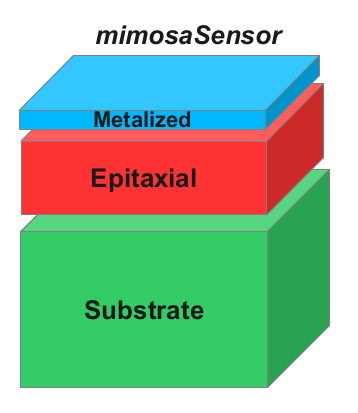
\includegraphics[scale=0.40]{./figures/couches_capteur.png}
      \caption{Diff\'erentes couches de la simulation d'un capteur CMOS.}
     \end{center}
    \end{figure}
    Dans notre simulation un capteur est construit gr\^ace \`a un assemblage de 3 couches de silicium : une couche de substrat, une couche épitaxiée et une couche de métallisation. Seule la couche épitaxiée est rendue sensible. La couche de substrat est \'epaisse de 36 $\mu m$, la couche \'epitaxi\'ee de 9 $\mu m$ et la couche d'oxyde et de m\'etal de 5 $\mu m$. L'épaisseur du capteur est alors de 50 $\mu m$. La longueur du \textit{step} dans la couche épitaxiée est \'egale \`a la longueur travers\'ee par la particule dans cette m\^eme couche. On notera que l'\'epaisseur de la couche \'epitaxi\'ee n'est pas de $15 \, \mu m$ comme pour le capteur MIMOSA-28. Nous verrons plus loin dans ce chapitre les raisons de ce choix.

    \medskip
    
    Comme nous l'avons d\'ej\`a vu pr\'ec\'edemment, la simulation de nos capteurs se base sur le capteur MIMOSA-28. Les capteurs simul\'es doivent ainsi poss\'eder 960 colonnes et 928 lignes. Comme le pas inter-pixel entre chaque pixel est de 20.7 $\mu m$, en hauteur comme en largeur, la largeur du capteur mesure $960 \times 20.7 = 19872 \, \mu m$ et la hauteur : $928 \times 20.7 = 19209.6 \,\mu m$.
    
    \medskip
    
    Chaque capteur peut être situ\'e dans l'espace de l'exp\'erience selon les coordonn\'ees de son centre $(X_{capteur}, Y_{capteur}, Z_{capteur})$ par rapport au r\'ef\'erentiel du volume \textit{World}. De plus le capteur mis en jeu peut être inclin\'e selon les axes Ox, Oy et Oz (d\'efinis par les dimensions du volume \textit{World}.). 
    
%     La g\'eom\'etrie et la position des capteurs sont r\'eglables dans les fichiers  : \textit{DigiCmosDetectorConstruction.cc} et \textit{mimosaSensor.cc}.
    
  \subsection{Pixels et num\'erisation}
  
  Afin de rendre compte des pixels et de la nature binaire de la sortie de notre capteur, le transport des charges vers les pixels puis la discrimination du signal collect\'e dans les pixels sont effectu\'es. Chacune des \'etapes conduisant au signal final d\'etecté dans chaque pixel seront d\'ecrites dans cette section. Nous partirons du d\'epôt d'\'energie le long de la couche épitaxiée puis nous transporterons les charges induites vers les pixels du capteur, ensuite, une fois le bruit pour chaque pixel ajout\'e, nous numériserons le signal de chaque pixel. Enfin, nous effectuerons une suppression de z\'ero.
   
   \medskip

   Pour de fines \'epaisseurs de silicium, comme celle de notre capteur CMOS ($50 \, \mu m$ pour l'ensemble du capteur, $15 \, \mu m$ pour la couche \'epitaxi\'ee) le d\'epôt de charge dans la mati\`ere suit une distribution de Landau (voir section \ref{sect:bethe_bloch}). Diff\'erentes mesures du signal r\'ecolt\'e dans les pixels des capteurs CMOS du groupe, ont montr\'e que la valeur la plus probable (MPV) du d\'epôt de charge le long de la couche \'epitaxi\'ee, pour des pions charg\'es et dot\'es d'une impulsion de l'ordre de 120 $GeV$, \'etait d'environ $80 \, e^-/\mu m$.  
  
   \begin{figure}[!htb]
    \begin{center} 
     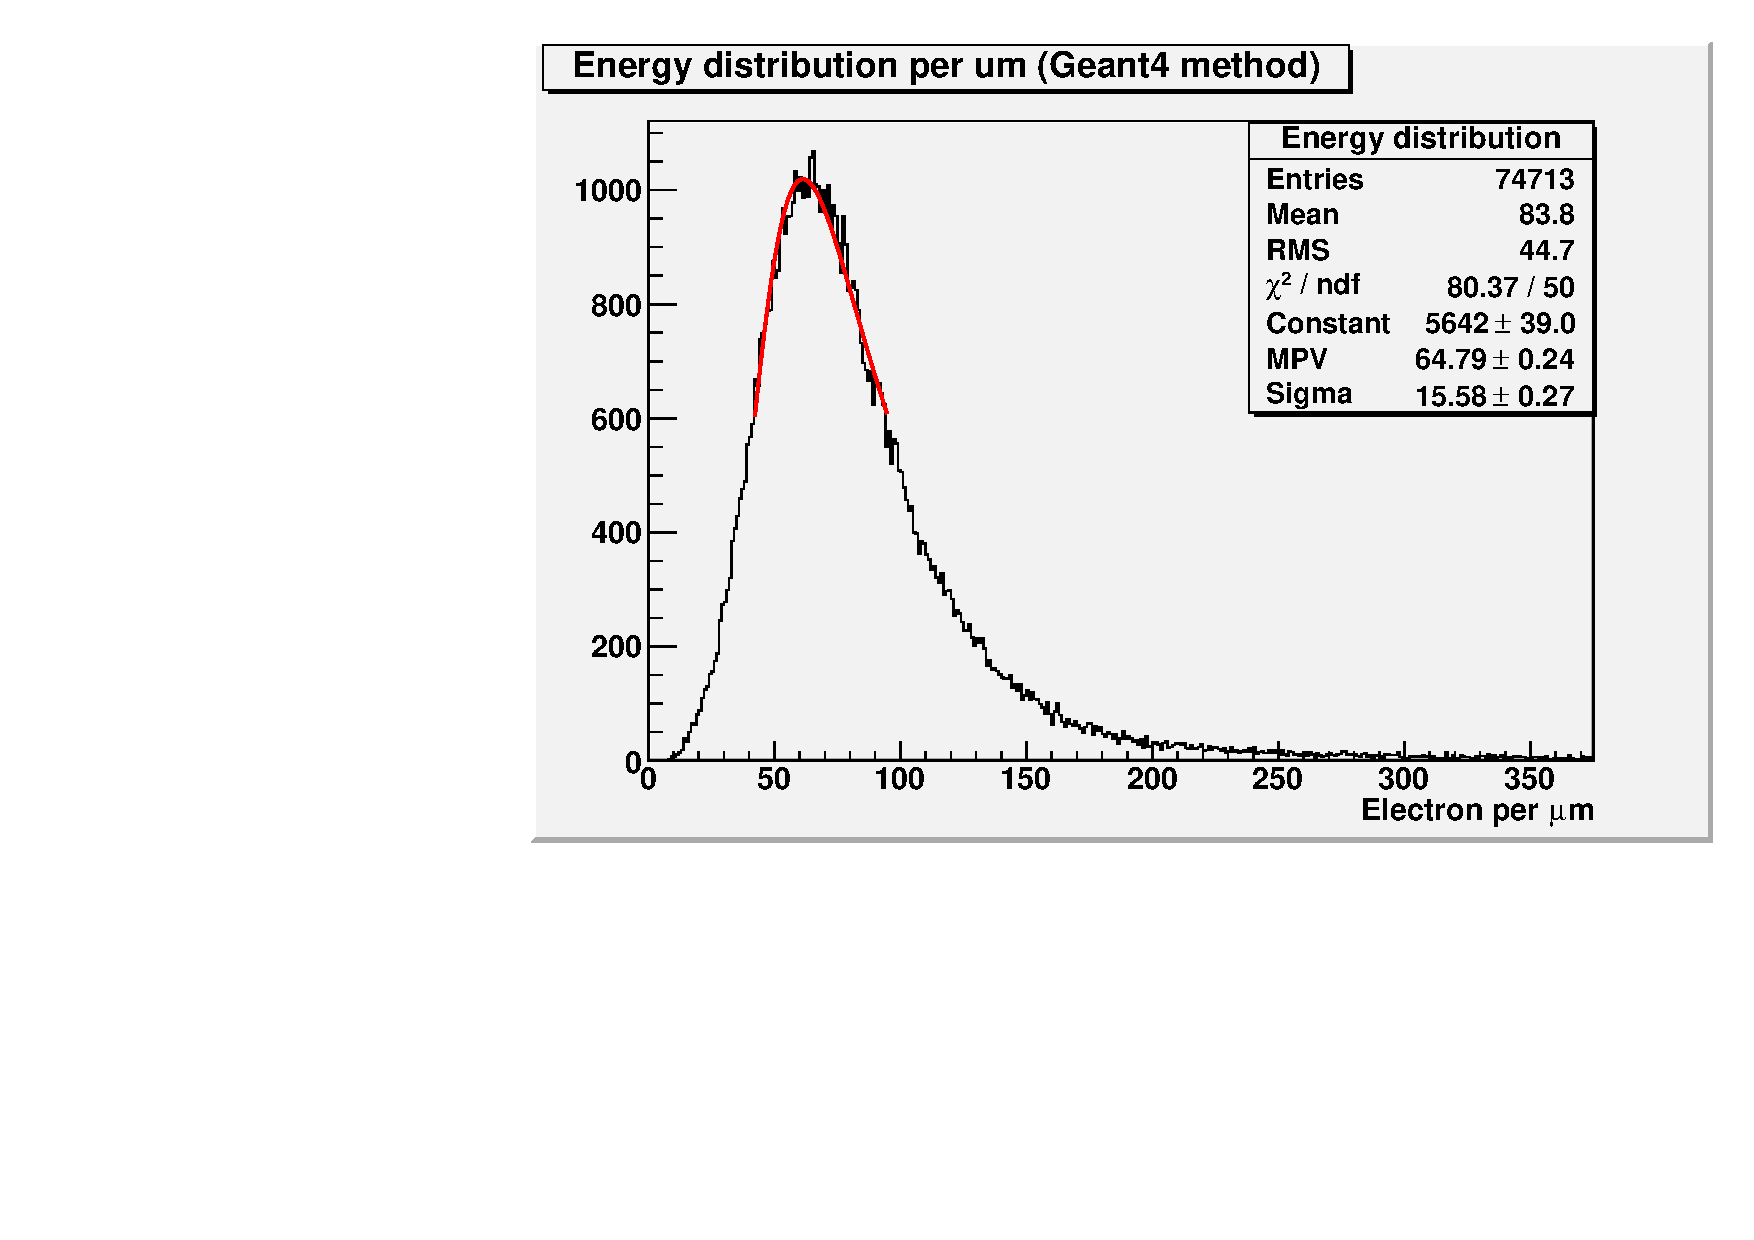
\includegraphics[scale=0.60]{./figures/energy_distrib_Geant4_3.pdf}
     \caption{\label{fig:distribEnergie} Distribution d'énergie par $\mu m$ dans GEANT4.}
    \end{center}
   \end{figure}

   \medskip
   
    Nous allons alors \'etudier la distribution du d\'epôt d'\'energie de \textit{GEANT4} pour une impulsion des pions de $120 GeV/c$ et une \'epaisseur de couche épitaxiée de $15 \mu m$. Cette distribution est visible en figure ~\ref{fig:distribEnergie}. Cette distribution n'est ni une distribution Gaussienne, ni une distribution de Laudau. En ajustant une distribution de Landau \`a cette distribution, la valeur la plus probable trouv\'ee est de $65 \, e^-/\mu m$. Afin d'obtenir une valeur la plus probable de $80 \, e^-/\mu m$ un facteur correctif de $1.25$ a \'et\'e ajout\'e. Comme la distribution du d\'epôt d'énergie n'est pas de type Landau mais s'en rapproche, l'ajout de ce facteur corrige essentiellement la zone autour de la valeur la plus probable. Les probabilit\'es pour de faibles d\'ep\^ots ($< 25 e^-/ \mu $m) ou de forts d\'ep\^ots ($> 125 e^-/ \mu m$) dans la mati\`ere restent quant \`a elles \'eloign\'ees des valeurs donn\'ees par une distribution de Landau.
    
    \medskip
    
    Une seconde option a \'et\'e de générer une distribution de dépôt d'\'energie \`a l'aide d'une distribution de Landau de MPV \'egale \`a $80 \, e^-/\mu m$ et d'une "largeur" (voir la d\'efinition de ROOT) proportionnelle \`a celle de la couche épitaxiée. Nous verrons dans la section résultats (\ref{sect:resultatsSIMU}) que notre choix pour le d\'epôt d'\'energie, s'est orient\'e vers cette distribution de Landau. Les r\'esultats obtenus avec celle-ci se rapprochant le plus de ceux des donn\'ees des tests en faisceau. 
   
    %depot energie dans la couche epitaxiale -> distribution de landau MPV $80 e^-/\mu m$  PAS GEANT4 -> Pourquoi ?\\
    %Plot Landau vs GEANT4 \\
  
    \subsubsection{Transport des charges}
 
    Le volume déserté autour des puits N \'etant r\'eduit et n'exc\'edant pas quelques $\mu m$ de profondeur (il  d\'epend en majeure partie de la r\'esistivit\'e de la couche épitaxiée), les porteurs de charge cr\'e\'es lors du passage de chaque particule \`a travers la couche épitaxiée sont essentiellement diffus\'es thermiquement. La plupart des porteurs de charge sont ainsi collect\'es par quelques diodes N-Well implant\'ees \`a la "surface" de la couche épitaxiée. Les pixels touch\'es forment alors un $amas$ de pixels. Un centre de gravit\'e sur celui-ci donne une r\'esolution sur l'impact meilleure que la r\'esolution digitale valant $\cfrac{pitch}{ \sqrt{12} }$. D'autres ph\'enom\`enes comme la recombinaison ou la r\'eflexion au niveau des interfaces plus fortement dop\'ees (substrat et zones P-Well) interviennent. 

   \begin{figure}[!Htb]
    \begin{center}
     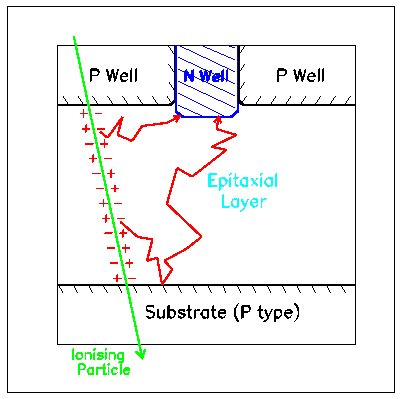
\includegraphics[scale=0.60]{./figures/cmos_principe.png}
     \caption{Diffusion des porteurs de charge.}
    \end{center}
    \label{fig:principeCMOS}
   \end{figure}
 
   \medskip
   
   La collection de charges d\'epend de plusieurs param\`etres non connus avec pr\'ecision tels que le profil de dopage et l'\'epaisseur de la couche épitaxiée. Ces contraintes nous am\`enent alors \`a utiliser un mod\`ele empirique bas\'e sur les donn\'ees recueillies lors des campagnes de tests en faisceau. Pour effectuer le transport des charges nous allons partir de l'hypoth\`ese que les charges sont uniform\'ement distribu\'ees selon le cheminement de la trace. Selon cette hypoth\`ese, le nombre de charges cr\'e\'ees $N$ est \'egal \`a l'\'energie $E_d$ d\'epos\'ee le long de la trajectoire de la particule charg\'ee dans la couche \'epitaxi\'ee, divis\'ee par l'\'energie d'ionisation du silicium $E_i = 3.6 \, eV$. On a ainsi :
   
   \begin{equation}
     N = \dfrac{E_d}{E_i}
   \end{equation}

  On peut alors d\'ecouper cette trace en $N$ segments, chaque segment contenant un \'electron. La charge se situera alors au milieu du segment consid\'er\'e. Afin de diminuer le temps de calcul, les $N$ \'electrons peuvent \^etre r\'epartis en $\cfrac{N}{k}$ segments, avec $k$ le nombre d'\'electrons par segment. Un nombre de $k=5$ \'electrons par segment r\'eduit le temps de calcul et n'impacte pas le r\'esultat final. Par la suite nous allons calculer la probabilit\'e pour qu'un \'electron distant d'une distance $d$ d'une diode N-Well soit collect\'e par celle-ci. Pour cela nous allons nous baser sur les donn\'ees des tests en faisceau.
 
   \begin{figure}[!htb]
    \begin{center} 
     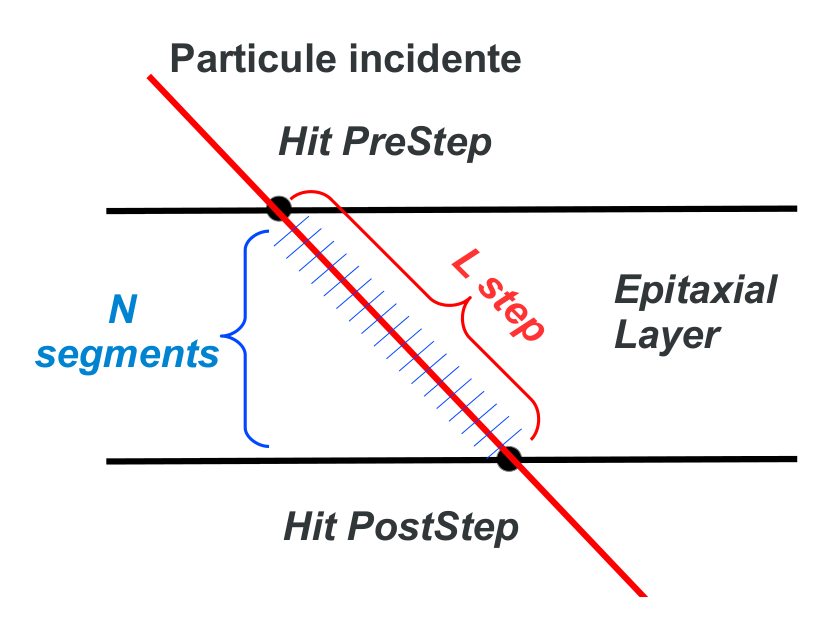
\includegraphics[scale=0.30]{./figures/segments.png}
     \caption{Segmentation de la trace.}
    \end{center}
    \label{fig:segments}
   \end{figure} 
   
   \medskip
   
   Lors d'un impact les charges lib\'er\'ees le long de la trajectoire dans la couche \'epitaxi\'ee vont se repartir pour former un amas. \`A incidence normale, cet amas ne d\'epasse pas en g\'en\'eral la taille de $5 \times 5$ pixels, la charge \'etant essentiellement r\'epartie dans le premier carr\'e de pixels autour de l'impact. Nous allons donc travailler dans le cas d'amas de $5 \times 5$ pixels maximum. La figure ~\ref{fig:cl5x5} illustre ce type d'amas. 
   

   \begin{figure}[!htb]
    \begin{center} 
     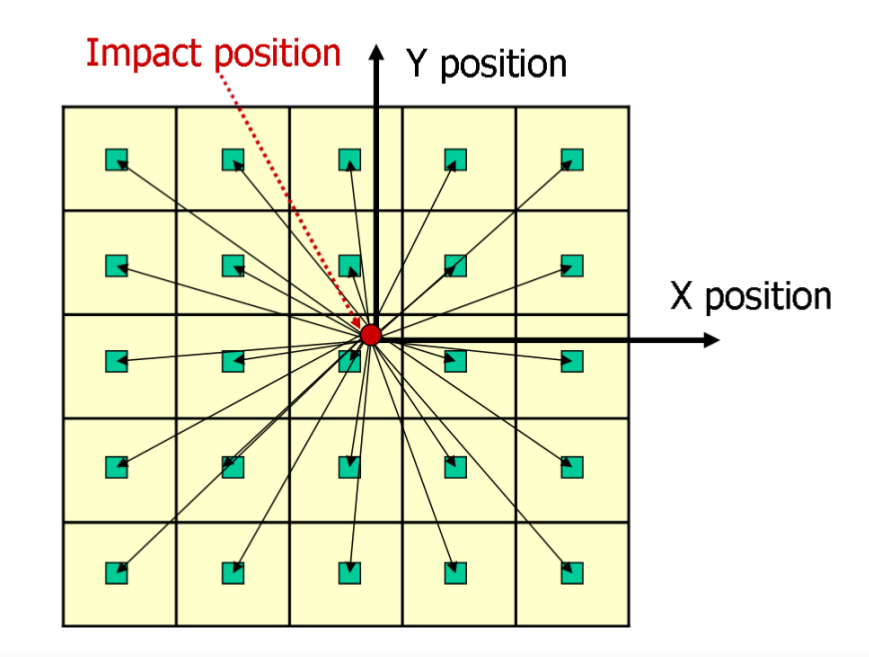
\includegraphics[scale=0.30]{./figures/5x5_cluster.png}
     \caption{Sch\'ema d'un amas $5 \times 5$ pixels.}
     \label{fig:cl5x5}
   \end{center}
   \end{figure}

   \medskip
   
   La premi\`ere \'etape de notre cheminement consiste \`a r\'ecup\'erer les charges collect\'ees par les pixels dans les donn\'ees du capteur analogique MIMOSA-22 AHR. Les charges re\c{c}ues dans chaque pixel de chaque amas sont lues pour tout les amas disponibles. Ensuite, pour chaque amas, les charges r\'ecolt\'ees dans les pixels de l'amas sont normalis\'ees par la charge totale reçue dans l'amas. La charge normalis\'ee de chaque pixel de chaque amas est ensuite rentr\'ee dans un histogramme \`a deux dimensions, avec en abscisse, la distance entre la position reconstruite de l'amas et la diode de collection du pixel dans le plan $XY$ du capteur, et en ordonn\'ee, la charge normalis\'ee. Cette op\'eration est effectu\'ee pour tous les impacts de l'\'ev\`enement et avec le maximum d'\'ev\`enements enregistr\'es possibles. Un exemple de cet histogramme (non normalis\'e) \`a deux dimensions est donn\'e en figure ~\ref{fig:plotcharge}. Pour chaque intervalle de distance, on calcule alors la charge normalis\'ee moyenne (voir figure ~\ref{fig:plotcharge}). On trouve ainsi un ensemble de points qui repr\'esentent la probabilit\'e pour une charge d'\^etre collect\'ee par une diode de collection d'un pixel situ\'e \`a une distance $d$ de la position de l'amas. Cette densit\'e de probabilit\'e a alors \'et\'e ajust\'ee avec un mod\`ele empirique.
   
   
   \begin{figure}[!htb]
    \begin{center} 
     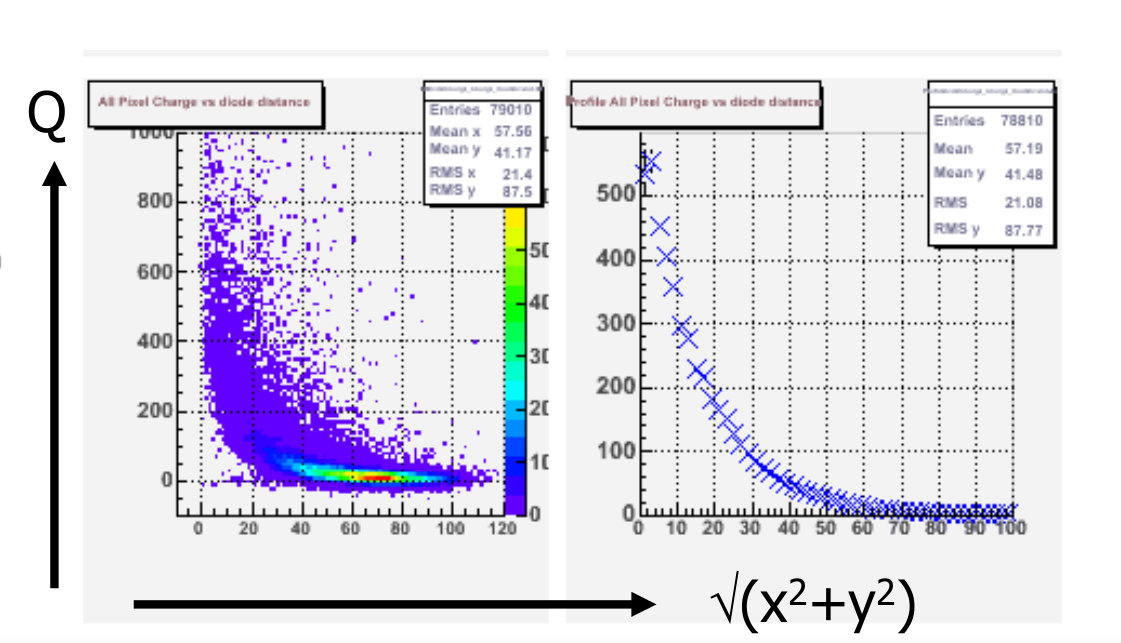
\includegraphics[scale=0.35]{./figures/plot_2D_charge_pdf.png}
     \caption{A gauche, histogramme \`a deux dimensions de la charge en $e^-$ en fonction de la distance (non normalis\'e). A droite, moyenne (non normalis\'ee) de la charge en $e^-$ moyen pour chaque intervalle de distance. }
     \label{fig:plotcharge}
     \end{center}
   \end{figure}

   Plusieurs formes de densit\'e de probabilit\'e ont \'et\'e essay\'ees. Notre choix s'est arr\^eté sur la somme d'une fonction Gaussienne avec une fonction Lorentzienne. La densit\'e de probabilit\'e s'exprime alors comme :
 
   \[ P(d) = N_0 \, e^{\frac{-(d-d_0)^2}{2\sigma^2}} + N_1 \, \frac{\Gamma}{\Gamma^2 + (d-d_1)^2} \]
   
   o\`u $d$ repr\'esente cette fois-ci la distance entre le centre du segment consid\'er\'e et la position de la diode ; et $N_0$, $\sigma$, $N_1$, $d_0$, $d_1$ et $\Gamma$ sont les param\`etres de l'ajustement. Pour l'ajustement une distinction a \'et\'e r\'ealis\'ee entre les pixels du premier carr\'e et les autres pixels de l'amas $5 \times 5$ que nous appellerons pixels externes. Cette distinction est r\'ealis\'ee \`a cause de l'effet d'\'ecrantage des pixels externes par les quatre pixels de la premi\`ere couronne. Cet effet est confirm\'e puisque nous obtenons de meilleurs r\'esultats en scindant ces deux groupes de pixels. Les param\`etres obtenus apr\`es ajustement sont r\'esum\'es dans le tableau ~\ref{tab:paramfit}.
   
  \begin{table}[h]
   \newcommand{\mc}[3]{\multicolumn{#1}{#2}{#3}}
    \begin{center}
     \begin{tabular}{|l|l|l|l|l|l|} \hline
      \mc{6}{|c|}{Pixels du premier carré}\\ \hline
      $N_0$ & $d_0$ & $\sigma$ & $\Gamma$ & $d_1$ & $N_1$\\ \hline
      0.458 & -3.98 & 13.2 & 3.99 & 1.80 & 6.45 \\ \hline
      \mc{6}{|c|}{Autres pixels}\\ \hline
      $N_0$ & $d_0$ & $\sigma$ & $\Gamma$ & $d_1$ & $N_1$\\ \hline
      0.117 & -1.07 & 17.5 & 47.1 & -4.64 & 3.71 \\ \hline
     \end{tabular}
   \end{center}
   \caption{Param\`etres de l'ajustement pour les pixels du premier carr\'e et pour les autres pixels d'un amas $5 \times 5$}
   \label{tab:paramfit}
  \end{table}
 
%    Pas de calcul de diffusion d'électron dans la couche épitaxiée car pas les donn`\'ees suffisantes (profil de dopage) \\
%    Probabilit\'e pour un électron d'être absorb\'e dans une diode -> A partir 
%    des tests en faisceau Mi22. \\
%    Deux cas \`a distinguer : Premi\`ere couronne et seconde couronne \\
%    Plots \\
%    Segmentation de la trace \\ 
%    Schéma segments \\
 
    \subsubsection{Ajout du bruit}
    
    Une fois le transport des charges effectu\'e, du bruit a \'et\'e ajout\'e. Pour cela chaque pixel s'est vu attribuer un bruit tir\'e dans une Gaussienne de largeur $13.7 \, e^-$.
   
    \medskip
    
    Afin de reproduire le taux d'impacts fant\^omes obtenu avec les donn\'ees des tests en faisceau, une \'etape suppl\'ementaire serait d'ajouter des pixels bruyants. Cette \'etape n'a pas \'et\'e r\'ealis\'ee lors de ce travail mais peut facilement \^etre ajout\'ee. %Nous ne reproduisons pas non plus le Bruit temporel \textit{TN} et le \textit{FPN}. Cependant, ces derniers peuvent \^etre reproduits en contaminant la sortie.
    
    \subsubsection{Digitisation et coupure en seuil}
   
    Afin d'obtenir une sortie équivalente au capteur MIMOSA-28, une numérisation du signal est effectu\'ee. Pour cela une fois la charge recueillie dans chaque pixel, \`a la façon d'un discriminateur, seuls les pixels possédants une valeur de charge au dessus d'un certain seuil sont conserv\'es. Les autres pixels sont rejet\'es. Le seuil appliqu\'e est choisi selon un multiple de la valeur moyenne du bruit (13.7 $e^-$). Différents seuils ont \'et\'e test\'es, ils s'échelonnent entre 4 et 12 fois la valeur moyenne du bruit. 
    
%     La numérisation est r\'ealis\'ee dans le fichier : \textit{DigiCmosDigitizer.cc}.
   
   \subsubsection{Sortie}
   
   A la sortie de notre simulation nous trouvons un fichier texte constitu\'e de diff\'erentes informations sur les pixels touch\'es. Une suppression de z\'ero a \'et\'e effectu\'ee et nous ne retrouvons que les pixels ayant pass\'es le seuil de la discrimination. Les informations contenues dans le fichier de sortie sont :
   
   \medskip
   
   \begin{itemize}
    \item Le num\'ero de l'\'ev\`enement
    \item Le num\'ero du capteur
    \item La ligne, la colonne et le num\'ero du pixel touch\'e.
    \item L'\'energie d\'epos\'ee dans le \textit{step} et l'\'energie transport\'ee dans le pixel
    \item Les coordonn\'ees Monte-Carlo du milieu du \textit{step} dans le rep\`ere du volume \textit{World}.
    \item Les inclinaisons des traces et leur point de d\'epart. (Facultatif : ajout en fin de th\`ese).
   \end{itemize}
   
   \medskip 
   
   Un fichier de configuration pour le programme d'analyse des donn\'ees nomm\'e TAF est aussi automatiquement g\'en\'er\'e en fonction de la g\'eom\'etrie de l'expérience simul\'ee. Il comporte le type de capteur utilis\'e et les informations de position et d'inclinaisons sur les capteurs, \'echelles et super-plans simul\'es utilis\'es.
   
  \subsubsection{Interface avec le programme de reconstruction des \'ev\`enements}
  
   Afin d'analyser les donn\'ees en sortie de la simulation, une interface avec le programme de reconstruction et d'analyse, TAF, a \'et\'e cr\'e\'ee. Celle-ci permet de lire les donn\'ees simul\'ees de l'ensemble des capteurs utilis\'es dans la simulation GEANT4. De plus, le programme GEANT4 produit un fichier de configuration sp\'ecifique de la g\'eom\'etrie simul\'ee pour le logiciel d'analyse \textit{TAF}. Il fournit au logiciel TAF les informations de positions et d'inclinaisons des capteurs, et les informations sur les caract\'eristiques des capteurs simul\'es (lignes, colonnes, taille de pixels, etc ..).  Le programme de reconstruction et d'analyse est alors pr\`es à lire et analyser les donn\'ees des capteurs simul\'es. La figure \ref{fig:softs} illustre l'ensemble de l'architecture logicielle utilis\'ee pour cr\'eer et analyser nos simulations.

   \begin{figure}[!htb]
     \begin{center} 
      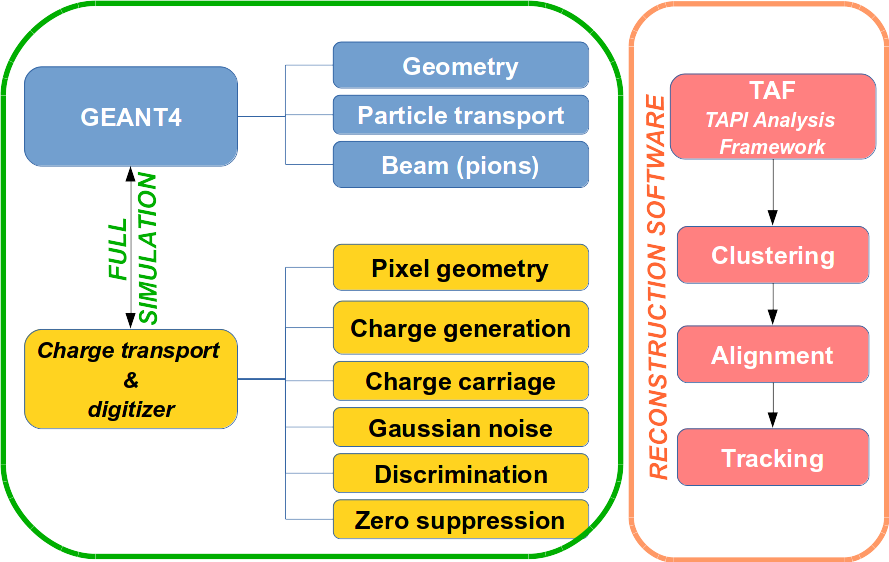
\includegraphics[scale=0.5]{./figures/Schema_framework_software.png}
      \caption{Architecture logicielle utilis\'ee pour la simulation (\textit{GEANT4}) et l'analyse de donn\'ees (\textit{TAF}).}
      \label{fig:softs}
     \end{center}
   \end{figure}
   
  \subsection{\'Echelles de capteurs CMOS et super-plan SALAT}
   
   Dans cette section nous allons voir de quelle fa\c{c}on sont r\'ealis\'ees les simulations d'objets constitu\'es \`a partir du capteur CMOS que nous avons simul\'e. Nous verrons ainsi la conception : d'\'echelles double face \textit{PLUME} et de super-plans \textit{SALAT}.
   
   \subsubsection{Géométrie d'une échelle type PLUME}
    
    Dans cette partie, nous allons voir comment une \'echelle PLUME est simul\'ee. \`A la diff\'erence d'une v\'eritable \'echelle PLUME, l'\'echelle PLUME simul\'ee dans cette th\`ese est constitu\'ee de capteurs MIMOSA-28 amincis \`a 50 $\mu m$ et non de capteurs MIMOSA-26. Le capteur analogique sur lequel se base MIMOSA-26 n'a pas \'et\'e autant \'etudié que MIMOSA-22 AHR. Pour cette raison nous n'avons pas pu obtenir un ajustement pr\'ecis du transport des charges. Ainsi, nous avons choisi de concevoir nos \'echelles \textit{PLUME} simul\'ees \`a l'aide de capteurs simul\'es MIMOSA-28.
    
    \medskip
    
    Pour construire une \'echelle \textit{PLUME} simul\'ee, 12 capteurs simul\'es MIMOSA-28, 6 par face, ont \'et\'e dispos\'es sur support d'\'epaisseur $2 \, mm$. Ce support est compos\'e d'une mousse de carbure de silicium $SiC$ de 1740 $\mu m$ d'\'epaisseur et de deux circuits imprim\'es de type kapton d'une \'epaisseur de 130 $\mu m$. Les deux supports de kapton sont compos\'es d'une \'epaisseur de 100 $\mu m$ de kapton englobant deux couches d'aluminium de 10 $\mu m$ d'\'epaisseur. Enfin, les capteurs sont coll\'es sur le kapton avec une couche de colle d'une \'epaisseur d'environ 10 $\mu m$. Un sch\'ema en coupe de l'\'echelle PLUME simul\'ees est donn\'e en figure \ref{fig:coupePLUME}. De plus, l'espace inter-capteur a \'et\'e fix\'e \`a 420 $\mu m$.
    
    \begin{figure}[!htb]
     \begin{center} 
      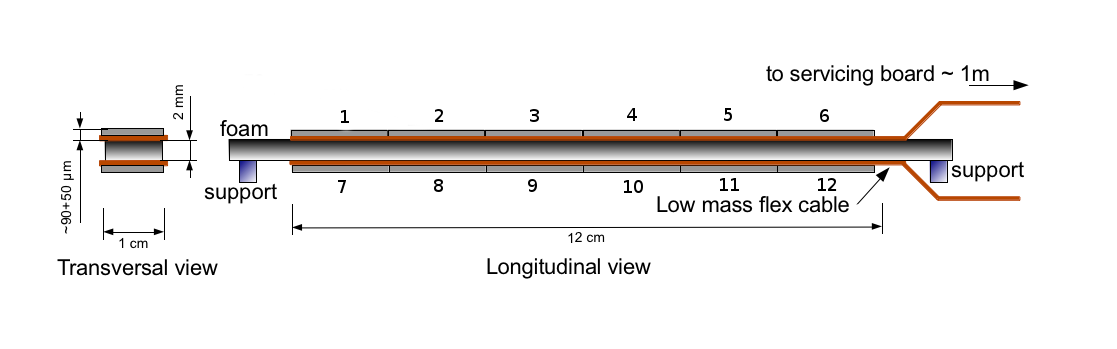
\includegraphics[scale=0.45]{./figures/plume_schema.png}
      \caption{Schéma d'une \'echelle PLUME.}
     \end{center}
    \end{figure}
    
    Les capteurs de l'\'echelle sont num\'erot\'es de 1 \`a 12. Les capteurs 1 \`a 6 sont les capteurs situ\'es sur la face avant de l'échelle ($z$ n\'egatifs sur le sch\'ema \ref{fig:coupePLUME}). Les capteurs 7 \`a 12 sont quant \`a eux plac\'es sur la face arri\`ere de l'\'echelle ($z$ positifs sur le sch\'ema \ref{fig:coupePLUME}).
%     Chaque capteur est plac\'e par rapport au centre de l'\'echelle, c'est-à-dire par rapport au centre du volume \textit{mousse} selon les coordonn\'ees suivantes : 

%     le capteur num\'ero 1 est situ\'e \`a gauche de l'\'echelle, les capteurs 2 \`a 5 le suivent jusqu'au capteur 6, situ\'e \`a l'extr\'emit\'e droite de l'\'echelle.
% Ils sont situ\'es de gauche \`a droite en regardant l'échelle par la face avant.

    
    \begin{figure}[!h]
     \begin{center} 
      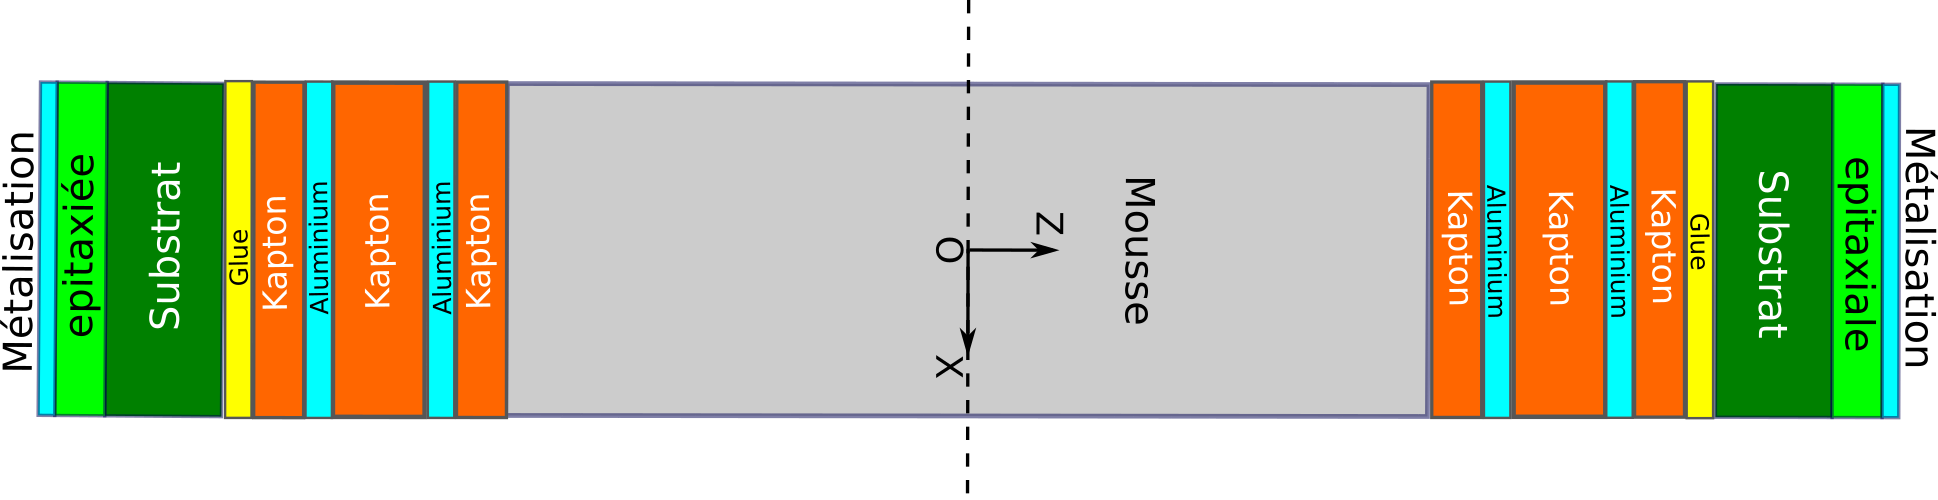
\includegraphics[scale=0.8]{./figures/PLUME_coupe.png}
      \caption{Coupe longitudinale d'une \'echelle PLUME, vue par la tranche. On peut y voir la mousse, les deux supports de type kapton et les capteurs CMOS.}
      \label{fig:coupePLUME}
     \end{center}
    \end{figure}
    
    \medskip
%     
%     Pour la face avant : 
%     
%     \begin{equation}
%      \left\{
%      \begin{array}{lll}
%          X = ( N - 3 - 0.5 ) \times (X_{capteur} + X_{inter \, capteur}) \, \mu m \\
%          Y = 0 \, \mu m \\
%          Z = - \cfrac{ Z_{support} }{2} - Z_{substrat} - \cfrac{ Z_{epi} }{2} - 5 = -1000 - 36 - 9/2 - 5 = -1045.5 \, \mu m 
%      \end{array}
%      \right.
%     \end{equation}
%     
%     
%     Pour la face arri\`ere : 
%     
%     \begin{equation}
%      \left\{
%      \begin{array}{lll}
%          X = ( N - 9 - 0.5 ) \times (X_{capteur} + X_{inter \, capteur}) \, \mu m \\
%          Y = 0 \, \mu m \\
%          Z = + \cfrac{ Z_{support} }{2} + Z_{substrat} + \cfrac{ Z_{epi} }{2} + 5 = 1000 + 36 + 9/2 + 5 = + 1045.5 \, \mu m 
%      \end{array}
%      \right.
%     \end{equation}  
%     
%     Avec $N$ le num\'ero du capteur, $X_{capteur}$ la largeur du capteur selon la coordonn\'ee $X$, $X_{inter \, capteur}$ la distance inter-capteur, $Z_{support}$ l'\'epaisseur du support, $Z_{substrat}$ l'\'epaisseur du substrat et $Z_{epi}$ l'\'epaisseur de la couche épitaxiée.
%     
%     \medskip
%     
%     Les $5 \, \mu m$ rajout\'es ou enlev\'es \`a la coordonn\'ee Z assurent que les volumes \textit{GEANT-4} ne s'interp\'en\`etrent pas.

   Le tableau \ref{tab:coordCapteurPLUME} r\'esume les coordonn\'ees des 12 capteurs par rapport au centre de l'\'echelle.
    
    \medskip
    
    \begin{table}[h]
    \footnotesize 
    \begin{center}
    \begin{tabular}{|l|l|l|l|} \hline
      Capteur & X ( $\mu m$ ) & Y ( $\mu m$ ) & Z ( $\mu m$ )\\ \hline
      1 & -53700 & 0 & -1045.5 \\ \hline
      2 & -30438 & 0 & -1045.5 \\ \hline
      3 & -10146 & 0 & -1045.5 \\ \hline
      4 & +10146 & 0 & -1045.5 \\ \hline
      5 & +30438 & 0 & -1045.5 \\ \hline
      6 & +53700 & 0 & -1045.5 \\ \hline
      7 & -53700 & 0 & +1045.5 \\ \hline
      8 & -30438 & 0 & +1045.5\\ \hline
      9 & -10146 & 0 & +1045.5\\ \hline
      10 & +10146 & 0 & +1045.5\\ \hline
      11 & +30438 & 0 & +1045.5\\ \hline
      12 & +53700 & 0 & +1045.5\\ \hline
    \end{tabular}
    \caption{Coordonn\'ees des capteurs par rapport au centre de l'\'echelle}
    \label{tab:coordCapteurPLUME}
    \end{center}
    \end{table}
    
   L'\'echelle peut ensuite \^etre dispos\'ee dans l'espace. Pour cela une transformation des coordonn\'ees de chaque \'el\'ement de l'\'echelle est effectu\'ee. La transformation est constitu\'ee de translations selon les directions $\overrightarrow{X}$,$\overrightarrow{Y}$ et $\overrightarrow{Z}$ et de rotations selon les axes Ox,Oy et Oz. 
   
%    La g\'eom\'etrie et la position des \'echelles PLUME sont r\'eglables dans les fichiers  : \textit{DigiCmosDetectorConstruction.cc} et \textit{ladderPLUME.cc}. Voyons \`a pr\'esent comment est simul\'e un super-plan \textit{SALAT}.
   
%    e \'echelle simple face.
   
%    \subsubsection{G\'eom\'etrie d'une \'echelle simple face}
%    
%    Les \'echelles simple face sont aussi simul\'ees \`a partir de la simulation du capteur MIMOSA-28. Six capteurs MIMOSA-28 simul\'es ont ainsi \'et\'e assembl\'es pour cette simulation. Aucun support n'a cependant \'et\'e utilis\'e, le but de cette simulation \'etant essentiellement de poss\'eder des donn\'ees pour développer un algorithme d'alignement d'\'echelles simple face. Une \'echelle simple face reprend les m\^emes caract\'eristiques qu'une face d'une \'echelle PLUME. On notera qu'un support peut tr\`es facilement \^etre ajout\'e. 
%    
%    \medskip
%    
%    Les capteurs de l'\'echelle sont dispos\'es selon les \'equations suivantes : 
%    
%    \begin{equation}
%      \left\{
%      \begin{array}{lll}
%          X = ( N - 3 - 0.5 ) \times (X_{capteur} + X_{inter \, capteur}) \, \mu m \\
%          Y = 0 \, \mu m \\
%          Z = - Z_{substrat} - \cfrac{ Z_{epi} }{2} - 5 = - 36 - 9/2 -5 = -45.5 \, \mu m 
%      \end{array}
%      \right.
%    \end{equation}
%     
%    L'espace inter-capteur $X_{inter \, capteur}$ est fix\'e \`a $X_{inter \, capteur} = 420 \mu m$. Une \'echelle simple face est sch\'ematis\'ee en figure \ref{fig:simple_face}.
% 
%     \begin{figure}[!h]
%      \begin{center} 
%       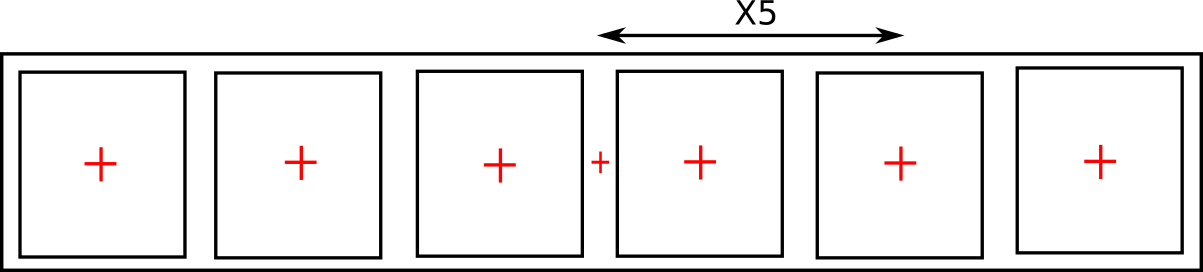
\includegraphics[scale=1.0]{./figures/fig_ech_simple_face.png}
%       \caption{Sch\'ema d'une \'echelle simple face. $X5$ est la position du capteur 5 de l'\'echelle simple face.}
%       \label{fig:simple_face}
%      \end{center}
%     \end{figure}
%    
%    Une fois la construction des \'echelles simple et double face d\'ecrite, nous allons d\'ecrire la conception d'une simulation d'un super-plan \textit{SALAT}.
   
   \subsubsection{G\'eom\'etrie d'un super-plan SALAT}
   
   La simulation d'un super-plan SALAT est r\'ealis\'ee \`a partir de la simulation du capteur MIMOSA-28. Pour cela, quatre capteurs MIMOSA-28 sont coll\'es \`a une feuille de Mylar d'\'epaisseur 50 $\mu m$. 
   
   \medskip
   
   Les capteurs sont num\'erot\'es de 1 \`a 4. La face avant du super-plan est d\'efinie par des coordonn\'ees $z$ n\'egatives et la face arri\`ere par des coordonn\'ees $z$ positives. Les capteurs 1 et 4 sont situ\'es sur la face avant ($z$ n\'egatifs). Le capteur 1 se situe en bas \`a gauche et le capteur 4 est plac\'e en haut \`a droite, lorsque l'on regarde le super plan par la face avant. Les capteurs 2 et 3 sont coll\'es \`a la face arri\`ere du super-plan ($z$ positifs). Le capteur 2 se situe en bas \`a droite alors que le capteur 3 se situe en haut \`a gauche lorsque l'on regarde le super-plan par la face avant.
    
    \begin{figure}[!htb]
     \begin{center} 
      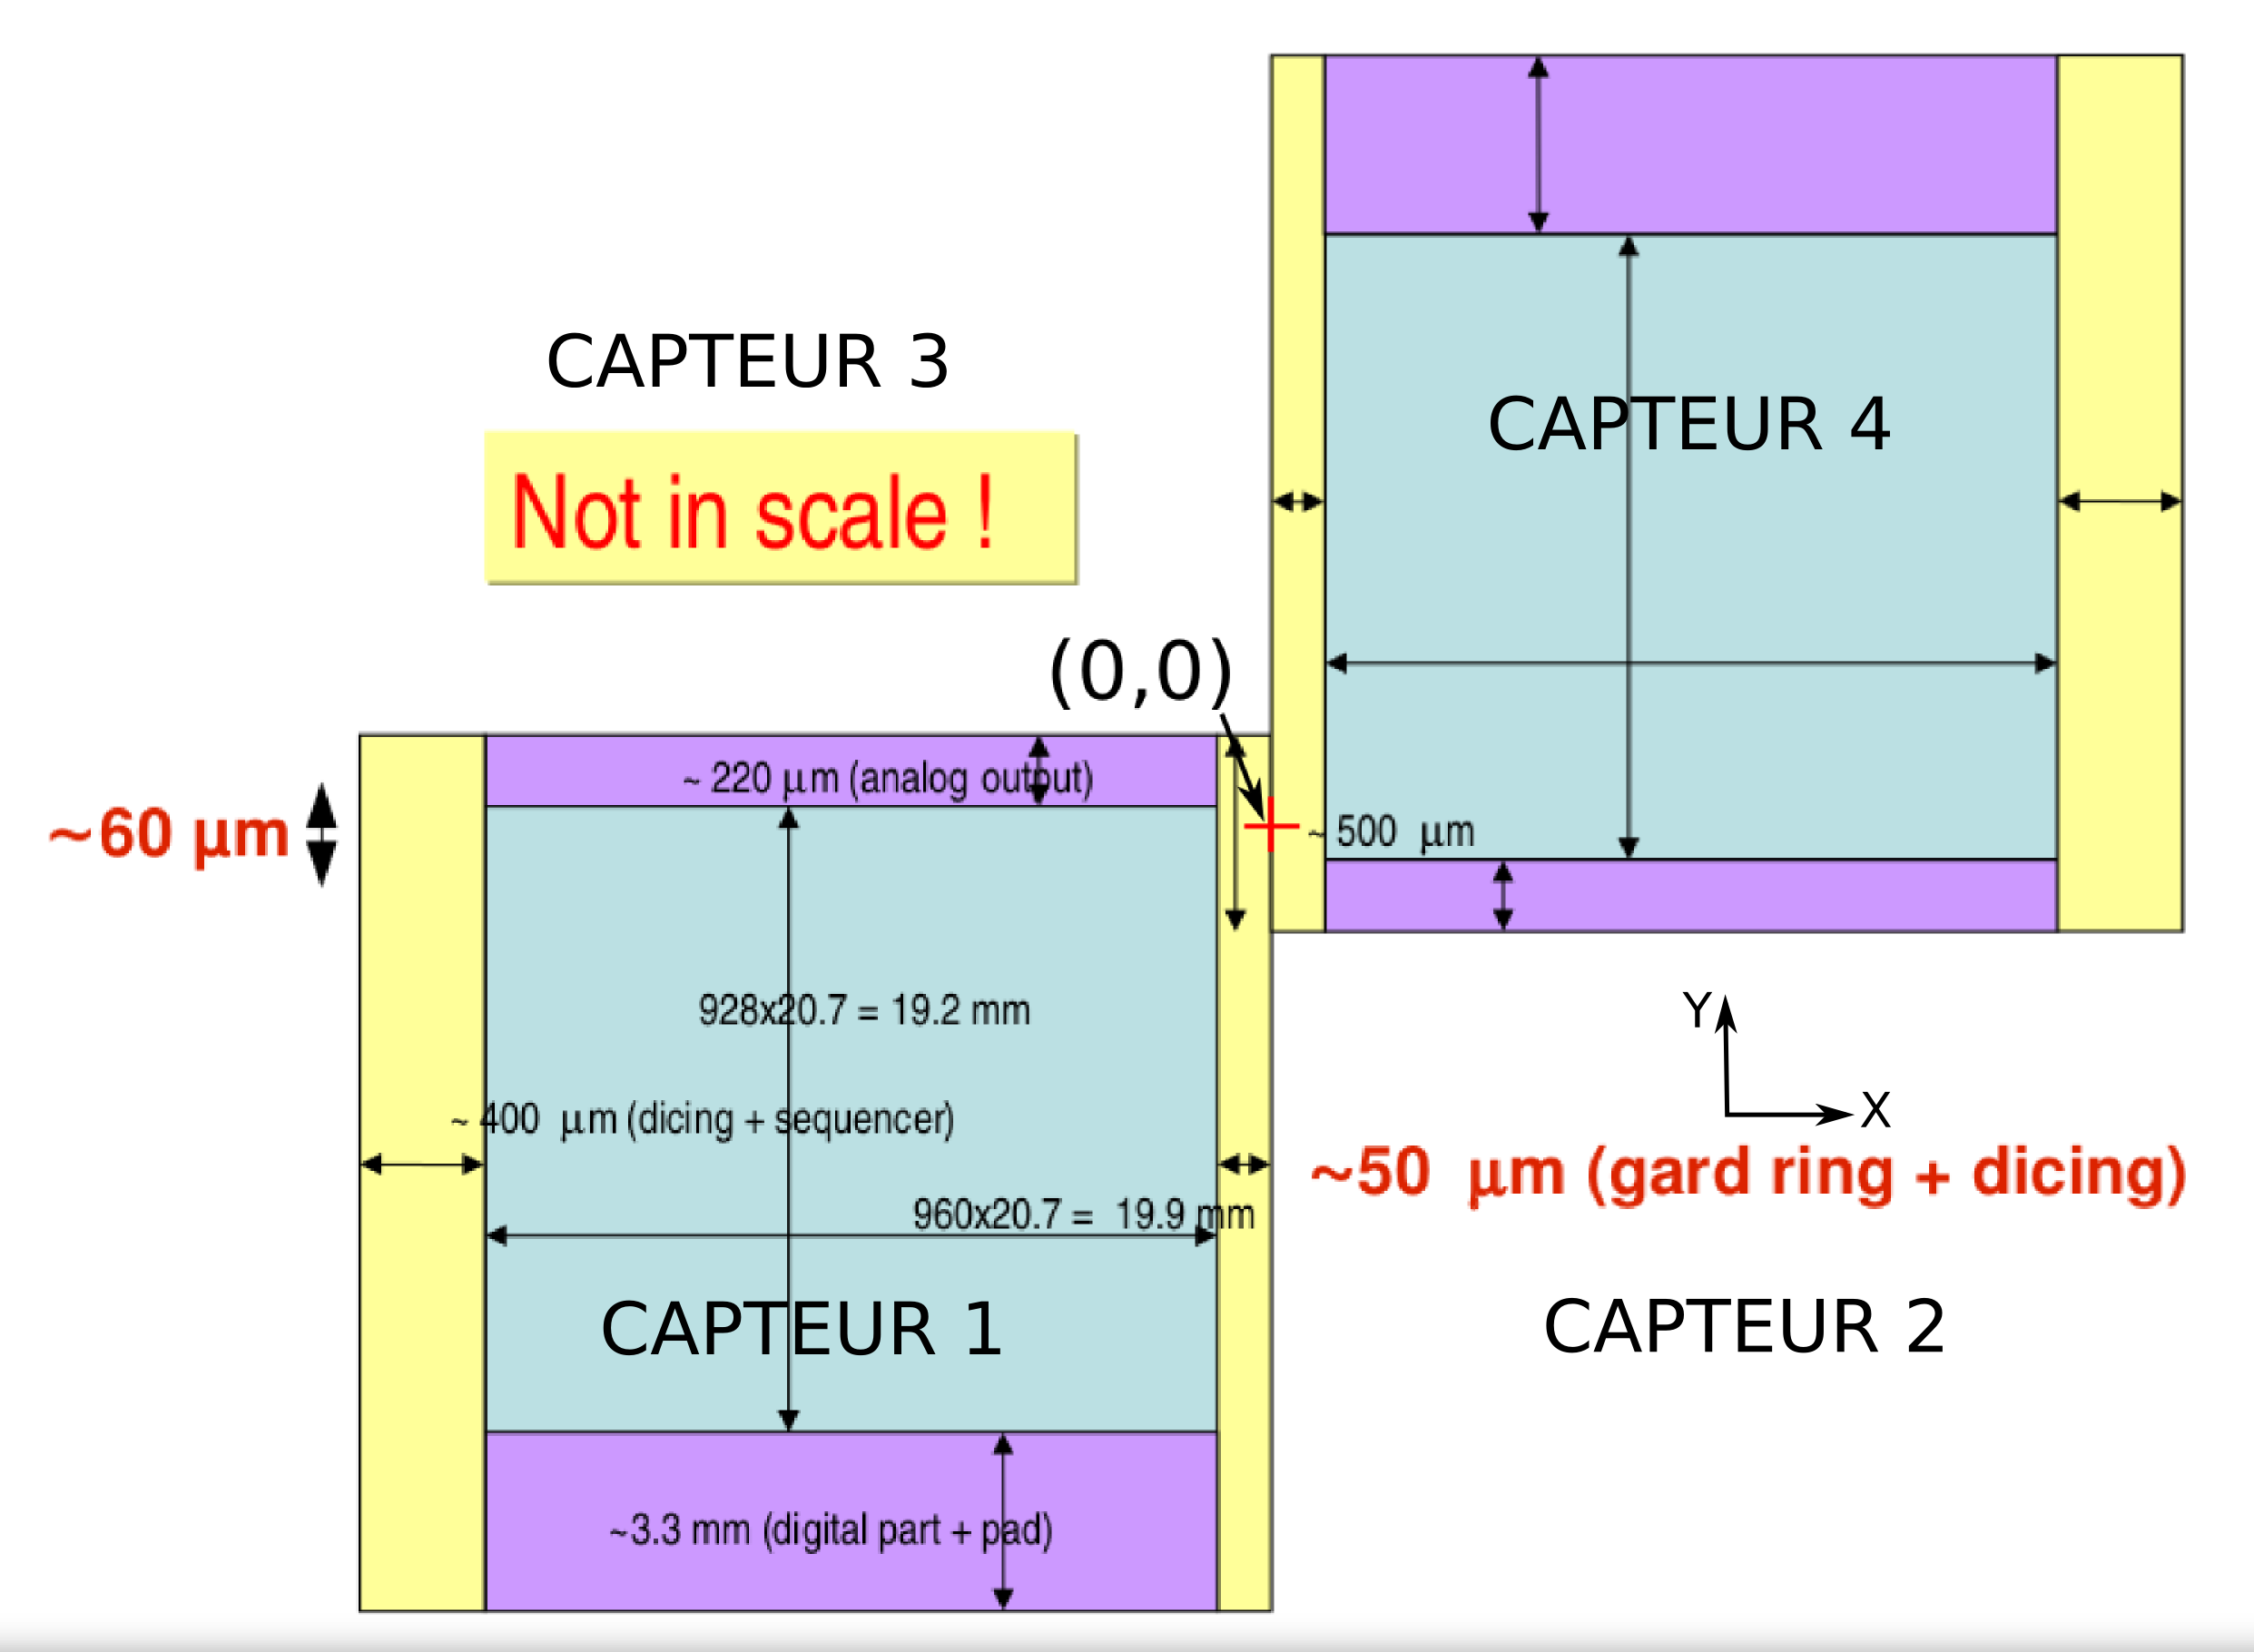
\includegraphics[scale=0.30]{./figures/SALAT_schema.png}
      \caption{Schéma d'un super plan SALAT, vu par la face avant.}
      \label{fig:coordCapteurSALAT0}
      \end{center}
    \end{figure} 
  
  \medskip
    
   La figure \ref{fig:coordCapteurSALAT0} montre la g\'eom\'etrie pour les deux plans de la face avant et montre la position des capteurs 2 et 3 situ\'es sur la face arri\`ere du super-plan. Comme indiqu\'e sur la figure \ref{fig:coordCapteurSALAT0} les capteurs 1 et 3 et 2 et 4 ont une zone de recouvrement selon l'axe Y de $60 \, \mu m$. De plus, les capteurs 1 et 2 et 3 et 4 sont distants de l'axe X de $\pm 50 \, \mu m$ par rapport au centre du super plan. 
   
%    
%    Chaque capteur est alors plac\'e par rapport au centre du super plan, c'est \`a dire par rapport au centre du volume en Mylar selon les coordonn\'ees suivantes :
%    
%    \medskip
%    
%    % first column
%    \begin{minipage}[t]{0.5\textwidth}
% 
%     Pour le capteur 1 : 
%     
%     \begin{equation}
%      \left\{
%      \begin{array}{lll}
%          X = -\left(\cfrac{X_{capteur}}{2}+50 \right) = -9986 \, \mu m \\
%          Y = -\left(\cfrac{Y_{capteur}}{2}-30 \right) = -9574,8 \, \mu m \\
%          Z =  \cfrac{Z_{Mylar}}{2} + \cfrac{Z_{Substrat}}{2} + \cfrac{Z_{Epi}}{2} + 5 \\
%          Z =  = 25+36+4.5+5 = 70.5 \, \mu m
%      \end{array}
%      \right.
%     \end{equation}
% 
%   \end{minipage}
%   %second column
%   \begin{minipage}[t]{0.5\textwidth}
% 
%    Pour le capteur 3 : 
%     
%     \begin{equation}     \left\{
%      \begin{array}{lll}
%          X = -\left(\cfrac{X_{capteur}}{2}+50 \right) = -9986 \, \mu m \\
%          Y = +\left(\cfrac{Y_{capteur}}{2}-30 \right) = +9574.8 \, \mu m \\
%          Z = -\left( \cfrac{Z_{Mylar}}{2} + \cfrac{Z_{Substrat}}{2} + \cfrac{Z_{Epi}}{2} + 5 \right) \\
%          Z = -70.5 \, \mu m 
%      \end{array}
%      \right.
%     \end{equation}
% 
% 
%   \end{minipage}      
% 
%    % first column
%    \begin{minipage}[t]{0.5\textwidth}
%    Pour le capteur 2 : 
%     
%     \begin{equation}     \left\{
%      \begin{array}{lll}
%          X = +\left(\cfrac{X_{capteur}}{2}+50 \right) = +9986 \, \mu m \\
%          Y = -\left(\cfrac{Y_{capteur}}{2}-30 \right) = -9574.8 \, \mu m \\
%          Z = \cfrac{Z_{Mylar}}{2} + \cfrac{Z_{Substrat}}{2} + \cfrac{Z_{Epi}}{2} + 5 \\
%          Z = +70.5 \, \mu m 
%      \end{array}
%      \right.
%     \end{equation}
% 
%   \end{minipage}
%   %second column
%   \begin{minipage}[t]{0.5\textwidth}  
%    Pour le capteur 4 : 
%     
%     \begin{equation}
%      \left\{
%      \begin{array}{lll}
%          X = -\left(\cfrac{X_{capteur}}{2}+50 \right) = -9986 \, \mu m \\
%          Y = -\left(\cfrac{Y_{capteur}}{2}-30 \right) = -9574.8 \, \mu m \\
%          Z = -\left( \cfrac{Z_{Mylar}}{2} + \cfrac{Z_{Substrat}}{2} + \cfrac{Z_{Epi}}{2} + 5 \right) \\
%          Z = -70.5 \, \mu m  
%      \end{array}
%      \right.
%     \end{equation}
% 
%   \end{minipage}
     
  \medskip
  
  Les positions des centres des trois capteurs selon l'axe $Oz$ sont espac\'ees du centre du super-plan d'une distance \'egale \`a la somme de la demi-\'epaisseur du volume en Mylar, de l'\'epaisseur du substrat du capteur, de la demi-\'epaisseur de couche \'epitaxi\'ee et de $5 \, \mu m$ de colle.
  
  \medskip
  
  Les positions et inclinaisons de chaque capteur dans le rep\`ere du super-plan sont r\'esum\'ees dans le tableau \ref{tab:coordCapteurSALAT} :
   
   \begin{table}[h]
   \begin{center}
   \begin{tabular}{|l|l|l|l|l|l|l|} \hline
   Capteur & X ( $\mu m$ ) & Y ( $\mu m$ ) & Z ( $\mu m$ ) & Ox ( $rad$ ) & Oy ( $rad$ ) & Oz ( $rad$ ) \\ \hline
   1 & $-9986$ & $-9574.8$ & $+70.5$ & 0 & 0 & 0 \\ \hline
   2 & $+9986$ & $-9574.8$ & $+70.5$ & 0 & $\pi$ & 0 \\ \hline
   3 & $-9986$ & $+9574.8$ & $-70.5$ & $\pi$ & 0 & 0 \\ \hline
   4 & $+9986$ & $+9574.8$ & $-70.5$ & $\pi$ & $\pi$ & 0 \\ \hline
   \end{tabular}
   \caption{Coordonn\'ees des capteurs par rapport au centre du super plan}
   \label{tab:coordCapteurSALAT}
   \end{center}
   \end{table}
   
   Le super plan SALAT peut ensuite \^etre dispos\'e dans l'espace gr\^ace \`a une transformation. La transformation est compos\'ee de trois translations selon les directions $\overrightarrow{X}$,$\overrightarrow{Y}$ et $\overrightarrow{Z}$ et de trois rotations selon les axes $Ox$, $Oy$ et $Oz$. La g\'eom\'etrie, la position et les inclinaisons des super-plans SALAT simul\'es sont r\'eglables dans les fichiers  : \textit{DigiCmosDetectorConstruction.cc} et \textit{salat.cc}.
   
  
   \section{R\'esultats}
   \label{sect:resultatsSIMU}

   Afin de tester notre simulation, nous allons la confronter aux donn\'ees des tests en faisceaux. Pour cela nous allons cr\'eer une simulation d'une exp\'erience avec un t\'elescope compos\'e de 4 plans MIMOSA-28 simul\'es et d'un DUT MIMOSA-28 simul\'e. Le t\'elescope form\'e est alors plac\'e dans un faisceau de pions n\'egatifs dot\'es d'une impulsion de 120 $GeV/c$. Les r\'esultats obtenus sont compar\'es \`a ceux du test en faisceau de MIMOSA-28 HR15 r\'ealis\'e en octobre 2011 au SPS avec un faisceau de pions charg\'es dot\'es de la même impulsion moyenne. Une fois les performances de notre simulation mises au jour et valid\'ees, nous \'etudierons les caract\'eristiques des simulations des \'echelles de capteurs PLUME et des super-plans SALAT.

% Cela n'influe cependant que de fa\c{c}on infime sur les r\'esultats puisque les variations d'impulsions du faisceau r\'eel sont faibles.
   
    \subsection{R\'esultats pour le capteur MIMOSA-28 simul\'e}
 
    \subsubsection{Faisceau de particule}
     
     Comme pour un test en faisceau r\'eel, le faisceau de particules utilis\'e pour cette simulation est un faisceau de pions n\'egatifs dot\'es d'une impulsion de 120 $GeV/c$. \`A la diff\'erence d'un faisceau r\'eel, tous les pions sont propag\'es avec une impulsion de pr\'ecis\'ement 120 $GeV/c$. La direction des pions suit l'axe $Oz$ de la simulation. Chaque pion est propag\'e \`a partir d'une surface de 4 $cm^2$ localis\'ee \`a la limite n\'egative du volume \textit{World} selon l'axe $Oz$ et centr\'ee en (0,0) selon les axes $Ox$ et $Oy$ de ce m\^eme volume.
     
     
    \subsubsection{G\'eom\'etrie du t\'elescope}  
   
   Le t\'elescope simul\'e comporte 4 plans de r\'ef\'erence MIMOSA-28 simul\'es et un \textit{DUT} MIMOSA-28 simul\'e. Chaque plan est distant l'un de l'autre d'une distance de 2 $cm$ selon l'axe $Oz$. Dans le plan $XY$, les capteurs sont centr\'es en $C_i(0,0,Z_i)$. La figure \ref{fig:geom_thr} illustre cette configuration. Les seuils des plans de r\'ef\'erence ont \'et\'e fix\'es \`a 8 $\sigma$. Le \textit{DUT} est le troisi\`eme capteur du t\'elescope et il est plac\'e en $z=0$.
   
   \begin{figure}[!htb]
    \begin{center} 
     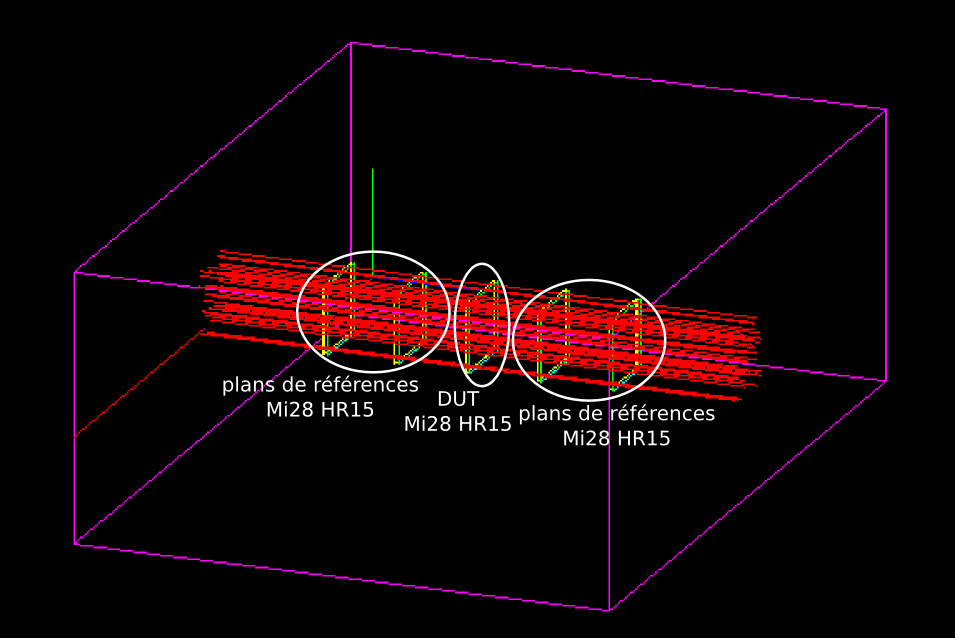
\includegraphics[scale=0.70]{./figures/geometrie_etude_thr.png}
     \caption{G\'eom\'etrie de l'exp\'erience avec 4 plans de r\'ef\'erences et un DUT affich\'e par \textit{GEANT4}.}
     \label{fig:geom_thr}
   \end{center}
   \end{figure}  
   
   \medskip
   
   Afin de calculer la r\'esolution du t\'elescope nous nous baserons sur la largeur de la distribution des r\'esidus lue sur le DUT au seuil de 8 $\sigma$. On a
   
   \begin{equation}
    \sigma_{Tel}^2 + \sigma_{DUT}^2 = \sigma_{Res}^2
   \end{equation}

   De plus au seuil de 8 $\sigma$ on a :
   
   \begin{equation}
    \sigma_{Tel} = \cfrac{\sigma_{Mi28}}{2}
   \end{equation}
   
   Et,
   
   \begin{equation}
    \sigma_{DUT} = \sigma_{Mi28}
   \end{equation}

   On obtient alors :
   
   \begin{equation}
    \sigma_{Mi28} = \sqrt{ \cfrac{4 \, \sigma_{Res}^2}{5} } 
   \end{equation}

   Et :
   
   \begin{equation}
    \sigma_{Tel} = \cfrac{\sigma_{Mi28}}{2} = \sqrt{ \cfrac{\sigma_{Res}^2}{5} }
    \label{eq:reso_tel_models}
   \end{equation}
   
   \subsubsection{Choix du mod\`ele de d\'ep\^ot de charge}

   Dans cette section, nous allons comparer les r\'esultats issus du d\'epôt de charge de \textit{GEANT4}, de deux d\'epôts de charge \textit{GEANT4} modifi\'es et du d\'epôt de charge de type \textit{Landau} avec les r\'esultats des tests en faisceau au SPS du capteur MIMOSA-28 HR15. Les deux mod\`eles \textit{GEANT4} modifi\'es correspondent \`a la multiplication du dépôt de charge de \textit{GEANT4} par un scalaire. Pour le premier mod\`ele dit modifi\'e, on modifie le d\'epôt de charge de \textit{GEANT4} pour obtenir une distribution du d\'epôt de charges avec une $MPV$ \'equivalente de 80 $e^-/\mu m$ (multiplication par $1.25$) et pour l'autre mod\`ele, on ajuste le d\'epôt de charge de \textit{GEANT4} pour reproduire la multiplicit\'e obtenue en test en faisceau (multiplication par $0.72$). Les r\'esultats de la simulation avec un d\'ep\^ot de charge de type \textit{Landau} sont obtenus avec une couche épitaxiée effective de $9 \, \mu m$ et avec une distribution de d\'ep\^ot d'\'energie suivant une distribution de \textit{Landau} de MPV 80 $e^-/\mu m$ et de "largeur" 15 fois la taille du \textit{step}. Nous choisirons par la suite le mod\`ele de d\'epôt de charge le plus en accord avec les donn\'ees r\'eelles et nous l'int\'egrerons \`a  notre simulation.
      
   \medskip
   
   La r\'esolution du télescope en $z=0$, l\`a o\`u se trouve le \textit{DUT} a \'et\'e estim\'ee pour les mod\`eles \textit{GEANT4}, \textit{GEANT4} modifi\'e, \textit{GEANT4} modifi\'e pour la multiplicit\'e et \textit{Landau} \`a respectivement environ 1.45, 1.625, 1.7 et 1.75 $\mu m$ ce qui correspond \`a des r\'esolutions spatiales pour un seuil de 8 fois le bruit de respectivement, 2.90, 3.25, 3.40 et 3.50 $\mu m$ pour les plans de r\'ef\'erence du t\'elescope. Ces r\'esolutions sont diff\'erentes en raison des r\'esolutions spatiales diff\'erentes obtenues pour chaque type de mod\`ele au seuil de 8 $\sigma$. Les r\'esolutions du t\'elescope en fonction du mod\`ele de d\'epôt de charge utilis\'e ont \'et\'e calcul\'ees \`a l'aide de la relation \ref{eq:reso_tel_models}
   
   \medskip
   
   \begin{figure}[!htb]
    \begin{center} 
     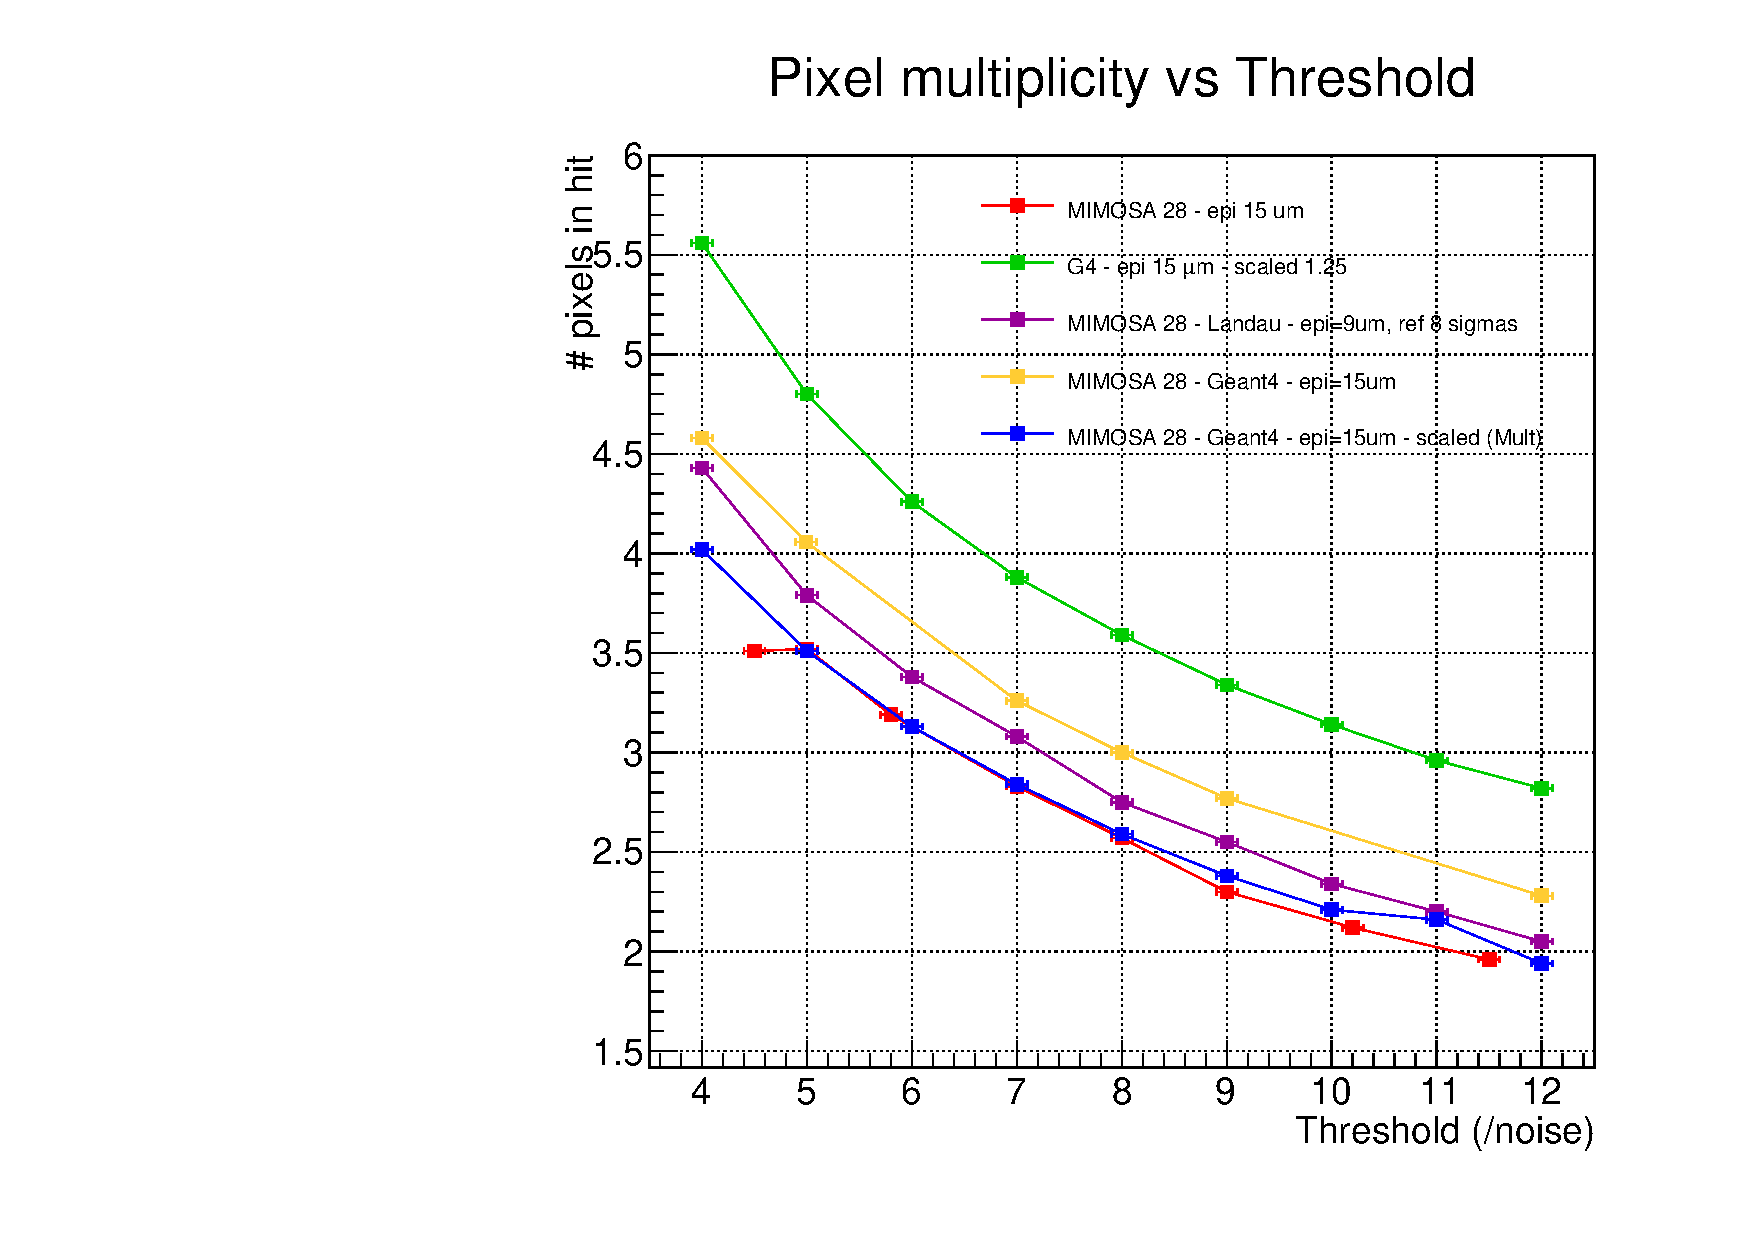
\includegraphics[scale=0.52]{./figures/Plots_resultat_simu/G4_landau_mult_oct.pdf}
     \caption{Multiplicit\'e moyenne des amas en fonction du seuil en multiple du bruit moyen. En rouge MIMOSA-28 HR15, le capteur de r\'ef\'erence. En violet, les r\'esultats avec le d\'epôt de charge de type \textit{Landau}. En orange, les r\'esultats de la simulation avec une couche épitaxiée de $15 \mu m$ et le d\'ep\^ot d'\'energie g\'en\'er\'e par \textit{GEANT4}. En vert, les r\'esultats de la simulation avec une couche épitaxiée de $15 \mu m$ et le d\'ep\^ot d'\'energie de \textit{GEANT4} modifi\'e. Et en bleu, le mod\`ele \textit{GEANT4} modifi\'e ajust\'e \`a la multiplicit\'e.}
    \label{fig:multiplicity}
    \end{center}
   \end{figure}
   
   La figure ~\ref{fig:multiplicity} illustre la multiplicit\'e moyenne des amas en fonction du type de d\'epôt d'\'energie dans la couche épitaxiée et du seuil en multiple du bruit moyen. La multiplicit\'e moyenne la plus \'elev\'ee est celle du mod\`ele GEANT4 modifi\'e avec une diff\'erence d'environ $+35$ \`a $+40$ $\%$ par rapport au capteur de r\'ef\'erence. Pour ce mod\`ele la multiplicit\'e moyenne varie entre environ $2.8$ et $5.6$ pixels par amas pour des seuils de 12 \`a 4 $\sigma$. Le mod\`ele \textit{GEANT4} donne une multiplicit\'e environ $15$ $\%$ plus \'elev\'ee que le capteur de r\'ef\'erence. La multiplicit\'e moyenne varie entre environ 2.8 pixels par amas pour un seuil de 12 $\sigma$ et 4.6 pixels par amas pour un seuil de 4 $\sigma$. Le mod\`ele de type Landau est lui plus \'elev\'e d'environ 10 $\%$ compar\'e aux donn\'ees des tests en faisceau. La multiplicit\'e moyenne varie alors entre 2.1 et 4.4 pixels par amas pour des seuils compris entre 12 et 4 $\sigma$. Enfin, la multiplicit\'e moyenne pour le mod\`ele \textit{GEANT4} modifi\'e pour la multiplicit\'e coïncide parfaitement, jusqu'au seuil de $8 \sigma$, avec la multiplicit\'e du capteur de r\'ef\'erence, au dessus de ce seuil la multiplicit\'e moyenne diffère sans toutefois atteindre une différence sup\'erieure \`a 10 $\%$. Cette multiplicit\'e moyenne varie entre 1.9 et 4.0 pixels par amas pour des seuils variant entre 12 et 4 $\sigma$. 
   
   \medskip
   
   Ces diff\'erences s'expliquent par les diff\'erents types de d\'epôts de charges dans la couche \'epitaxi\'ee. On rappelle que nous distribuons uniform\'ement les charges lib\'er\'ees selon la trajectoire de la trace dans la couche \'epitaxi\'ee (en 2 dimensions). Deux ph\'enom\`enes entrent alors en jeu. Premi\`erement, pour un type de d\'epôt de charges identique (\textit{GEANT4} par exemple), plus le d\'epôt moyen dans la couche \'epitaxi\'ee est important plus la multiplicit\'e sera \'elev\'ee. C'est ce que l'on observe sur la figure \ref{fig:multiplicity}. De plus, plus la charge d\'epos\'ee est \'eloign\'ee de la diode de collection de charge, plus le libre parcours de celle-ci a des chances d'\^etre important. Ainsi, plus les charges sont lib\'er\'ees en profondeur, plus l'\'etalement a des chances d'\^etre important. En moyenne, plus la couche \'epitaxi\'ee est \'epaisse plus la multiplicit\'e augmente (jusqu'\`a une certaine limite).
   
   \begin{figure}[!htb]
    \begin{center} 
     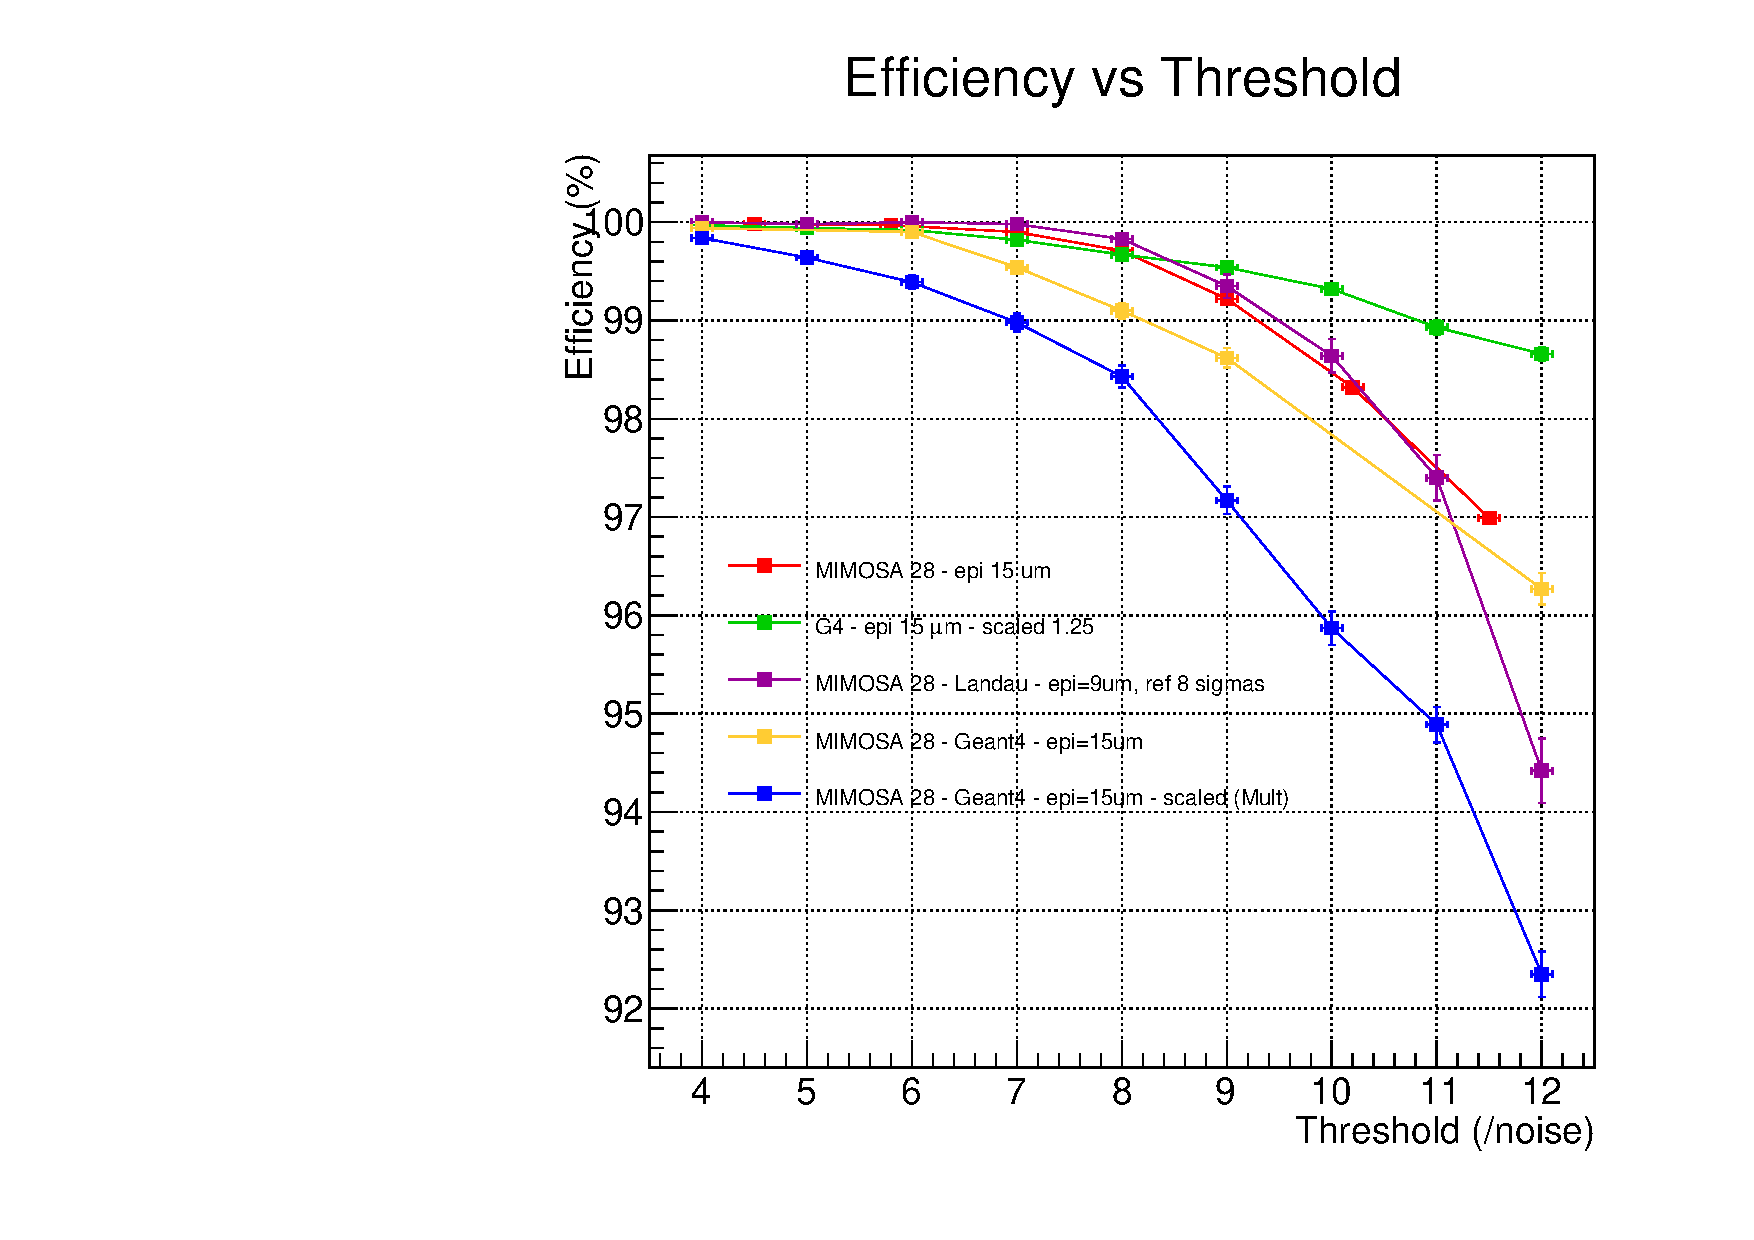
\includegraphics[scale=0.52]{./figures/Plots_resultat_simu/G4_landau_eff_oct.pdf}
     \caption{Efficacit\'e en fonction du seuil en multiple du bruit moyen. En rouge MIMOSA-28 HR15, le capteur de r\'ef\'erence. En violet, les efficacit\'e pour le mod\`ele \textit{Landau}. En orange, les efficacit\'e pour le mod\`ele \textit{GEANT4}. En vert, les efficacit\'e pour le mod\`ele \textit{GEANT4} modifi\'e ($\times 1.25$). Et en bleu le mod\`ele \textit{GEANT4} modifi\'e pour la multiplicit\'e.}
    \label{fig:efficiency}
    \end{center}
   \end{figure} 
   
   \medskip
   
   La figure \ref{fig:efficiency} illustre l'efficacit\'e de d\'etection en fonction du type de d\'epôt d'\'energie dans la couche épitaxiée et du seuil en multiple du bruit moyen. L'efficacit\'e pour le mod\`ele  GEANT4 modifi\'e pour la multiplicit\'e est la plus basse et ne coïncide pas avec les donn\'ees des tests en faisceau. Elle varie de $99.85\%$ pour un seuil de 4 $\sigma$ \`a $92.35\%$ pour un seuil de 12 $\sigma$. Pour le mod\`ele GEANT4, l'efficacit\'e coïncide avec les donn\'ees jusqu'à un seuil de 6 $\sigma$. Au dessus de ce seuil l'\'ecart entre le capteur de r\'ef\'erence et le mod\`ele GEANT4 devient important. On passe ainsi de $99.95\%$ \`a $96.3\%$ pour des seuils variant 4 et 12 $\sigma$. Le mod\`ele de type Landau coïncide avec les donn\'ees des tests en faisceaux jusqu'au seuil de 11 $\sigma$. Au delà, l'\'ecart s'agrandit. Pour ce mod\`ele, l'efficacit\'e est au dessus de $99.8\%$ pour des valeurs de seuil sup\'erieures ou \'egales \`a 8 $\sigma$. Enfin l'efficacit\'e du mod\`ele \textit{GEANT4} modifi\'e co\"incide entre 4 et 8 $\sigma$ avec l'efficacit\'e du capteur de r\'ef\'erence. Au-delà du seuil de 8 $\sigma$, l'efficacit\'e devient plus importante que celle du capteur de r\'ef\'erence. L'efficacit\'e pour ce mod\`ele vaut ainsi $98.65\%$ pour le seuil de 12 $\sigma$. Celle pour le capteur de r\'ef\'erence varie entre $99.98\%$ et $97.00\%$ entre les seuils de 4.5 et 11.5 $\sigma$. Ainsi, seul le mod\`ele de type \textit{Landau} poss\`ede une efficacit\'e proche de celle du capteur de r\'ef\'erence sur l'ensemble des seuils variant entre et 4 et 11 $\sigma$.
   
   \medskip
   
   Pour expliquer ce comportement, on effectue le m\^eme raisonnement que pour la multiplicit\'e. Seulement cette fois-ci, il y a un effet de seuil sur la charge collect\'ee par un pixel. Ainsi, plus la quantit\'e de charge d\'epos\'ee est importante, plus la quantit\'e de charges collect\'ee dans le pixel si\`ege est importante. Cette quantit\'e de charge doit alors passer le seuil du discriminateur pour allumer le pixel. Un seul pixel allum\'e (le pixel si\`ege) est suffisant pour identifier le passage d'une particule. La forme de la distribution du d\'epôt de charge et sa valeur moyenne est donc tr\`es importante dans ce cas. Par exemple, lorsque la distribution de charge est tr\`es large, m\^eme si la valeur moyenne est \'elev\'ee, de faibles d\'ep\^ots de charges dans la couche \'epitaxi\'ee sont possibles. \`A cause des ces faibles d\'ep\^ots, l'efficacit\'e peut chuter, m\^eme si les valeurs du d\'epôt de charges au dessus de la moyenne sont assez \'elev\'ees pour passer le seuil du pixel si\`ege. Ainsi, dans notre cas une distribution de \textit{Landau} de "largeur" ajust\'ee est la plus adapt\'ee.
   
   \begin{figure}[!htb]
    \begin{center} 
     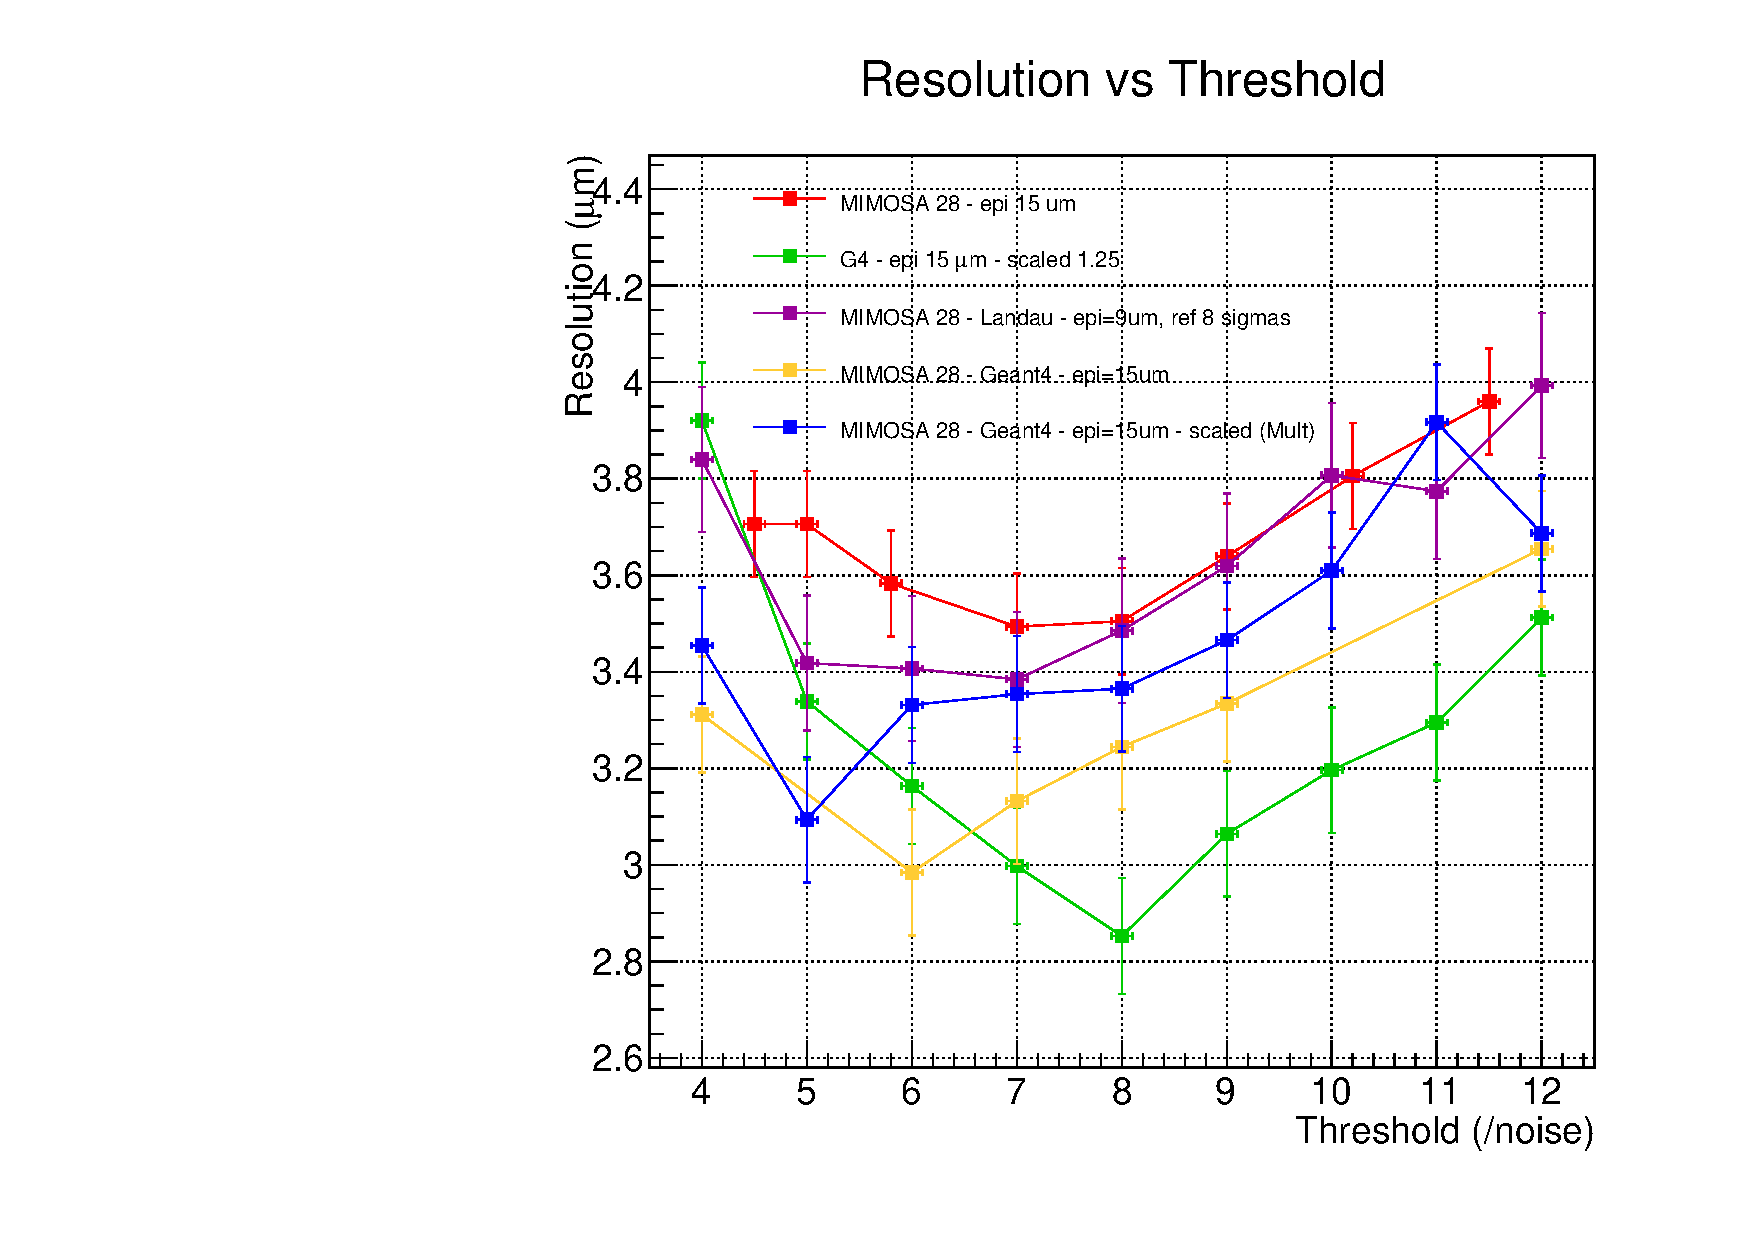
\includegraphics[scale=0.52]{./figures/Plots_resultat_simu/G4_landau_res_oct.pdf}
     \caption{R\'esolutions en fonction du seuil en multiple du bruit moyen. En rouge MIMOSA28 HR15, le capteur de r\'ef\'erence. En violet, les r\'esolutions pour le mod\`ele de type \textit{Landau}. En orange, les r\'esolutions pour le mod\`ele GEANT4. En vert, les r\'esolutions pour le mod\`ele GEANT4 modifi\'e. Et en bleu les r\'esolutions pour le mod\`ele \textit{GEANT4} modifi\'e pour la multiplicit\'e.}
    \label{fig:resolution}
    \end{center}
   \end{figure} 
   
   \medskip
   
   La figure \ref{fig:resolution} repr\'esente la r\'esolution spatiale en fonction du type de mod\`ele de d\'ep\^ot de charge et du seuil des discriminateurs en multiple du bruit moyen. Ces r\'esolutions sont compar\'ees avec les donn\'ees du capteur MIMOSA-28 HR15 obtenues lors des tests en faisceau. Les r\'esolutions en fonction du seuil des discriminateurs du capteurs obtenus pour le mod\`ele \textit{GEANT4} modifi\'e pour la multiplicit\'e ne co\"incident pas avec celles du capteur de r\'ef\'erence. Les multiplicit\'es obtenues pour ce mod\`ele sont inf\'erieures d'environ 0.1 \`a 0.5 $\mu m$ \`a celles du capteur de r\'ef\'erence malgr\'e des valeurs de multiplicit\'es moyennes des amas identiques. Cela s'explique par des distributions de multiplicit\'es diff\'erentes mais partageant la m\^eme valeur moyenne. Cela explique aussi que la valeur minimale de la multiplicit\'e n'est pas obtenue au m\^eme seuil (7 $\sigma$ pour la r\'ef\'erence et 5 $\sigma$ pour le mod\`ele \textit{GEANT4} modifi\'e pour la multiplicit\'e). Les r\'esolutions obtenues pour les mod\`eles \textit{GEANT4} et \textit{GEANT4} modifi\'e sont aussi en dessous des valeurs de r\'ef\'erences. Les diff\'erences atteignent jusqu'\`a respectivement 0.5 et 0.6 $\mu m$ au niveau des minimums de r\'esolution de ces deux mod\`eles correspondant aux seuils de 6 et 8 $\sigma$. On ne reviendra pas plus en d\'etail sur ces deux mod\`eles. Le mod\`ele de type Landau est celui qui se rapproche le plus de la r\'esolution obtenue lors des tests en faisceau de MIMOSA-28. Les valeurs de r\'esolution sont compatibles aux erreurs pr\`es entre 4 et 12 $\sigma$ avec des valeurs de r\'esolution variant entre 3.4 et 4.0 $\mu m$. Pour ce mod\`ele la r\'esolution \`a 4 $\sigma$ vaut 3.9 $\mu m$, puis cette r\'esolution diminue jusqu'à son minimum valant 3.4 $\mu m$ obtenu pour un seuil de 7 $\sigma$. \`A plus haut seuil, la r\'esolution augmente en suivant celle du capteur de r\'ef\'erence jusqu'\`a atteindre 4.0 $\mu m$ pour le seuil de 12 $\sigma$
   
%    Cette r\'esolution est la plus basse pour un mod\`ele de dépôt d'\'energie de type GEANT4, avec un écart variant entre 0.25 \`a 8 $\sigma$ et 0.6 $\mu m$ \`a 6 $\sigma$ pour des valeurs de r\'esolution comprises entre 3.0 et 3.7 $\mu m$. Pour le mod\`ele de type GEANT4 modifi\'e, la r\'esolution spatiale est plus \'elev\'ee que celle de du mod\`ele GEANT4 mais reste en dessous de celle du capteur de r\'ef\'erence d'environ 0.1 \`a 0.2 $\mu m$ entre 6 et 10 $\sigma$ en atteignant des valeurs respectivement comprises entre 3.4 et 3.6 $\mu m$. Pour 4 et 5 $\sigma$ la valeur de la r\'esolution vaut environ $3.1$ et $3.5$. Chiffres \`a comparer \`a la valeur du capteur de r\'ef\'erence pour un seuil de 5 $\sigma$ : environ 3.7 $\mu m$. \`A 11 sigma la valeur de la r\'esolution se confond avec celle du capteur de r\'ef\'erence en atteignant une valeur de 3.9 $\mu m$. Puis \`a 12 $\sigma$ la valeur de r\'esolution pour le mod\`ele GEANT4 modifi\'e, chute \`a $3.7$ $\mu m$. Le mod\`ele de type Landau est celui qui se rapproche le plus de la r\'esolution obtenue en faisceaux tests. Les valeurs de r\'esolution sont compatibles entre 6 et 12 $\sigma$ avec des valeurs de r\'esolution variant entre 3.4 et 4.0 $\mu m$. A 5 $\sigma$ la valeur obtenue pour la r\'esolution spatiale est de 3.4 $\mu m$ alors qu'elle est de 3.7 $\mu m$ pour le capteur de r\'ef\'erence. Enfin, pour ce type de d\'epôt de charge, \`a 4 $\sigma$, la valeur obtenue est de 3.85 $\mu m$.
   
   \medskip  
    
   \ A la vue de ces r\'esultats, le mod\`ele de d\'epôt de charge choisi est le mod\`ele de type Landau. Il s'agit en effet du meilleur compromis en terme de multiplicit\'e des amas de pixels, d'efficacit\'e de d\'etection et de r\'esolution spatiale. Nous allons voir par la suite quel est le meilleur compromis pour ce type de d\'epôt de charges.
   
   \subsubsection{Choix de l'\'epaisseur de couche épitaxiée pour un mod\`ele de type Landau.}
   
   Pour le mod\`ele de d\'epôt de charge de type Landau, diff\'erentes \'epaisseurs de couches épitaxiées et diff\'erentes "largeurs" ont \'et\'e essayées. Nous pr\'esentons ici les r\'esultats pour des couches épitaxiées allant de 8 \`a 10 $\mu m$ par pas de 1 $\mu m$ et pour une "largeur" (voir d\'efinition de la Landau dans le logiciel \textit{ROOT}) de 15 fois la longueur du \textit{step}. Apr\`es diff\'erents essais avec des largeurs variables, une largeur de 15 fois la longueur du \textit{step} a \'et\'e jug\'ee optimale. La r\'esolution du télescope en $z=0$, l\`a ou se trouve le \textit{DUT}, a \'et\'e estim\'ee pour des couches épitaxiées de 8, 9 et 10 $\mu m$ \`a respectivement environ 1.80, 1.75 et 1.65 $\mu m$ ce qui correspond \`a des r\'esolutions pour les capteurs de r\'ef\'erence r\'egl\'es au seuil de 8 fois le bruit de respectivement, 3.6, 3.5 et 3.3 $\mu m$.

   \begin{figure}[!htb]
    \begin{center} 
     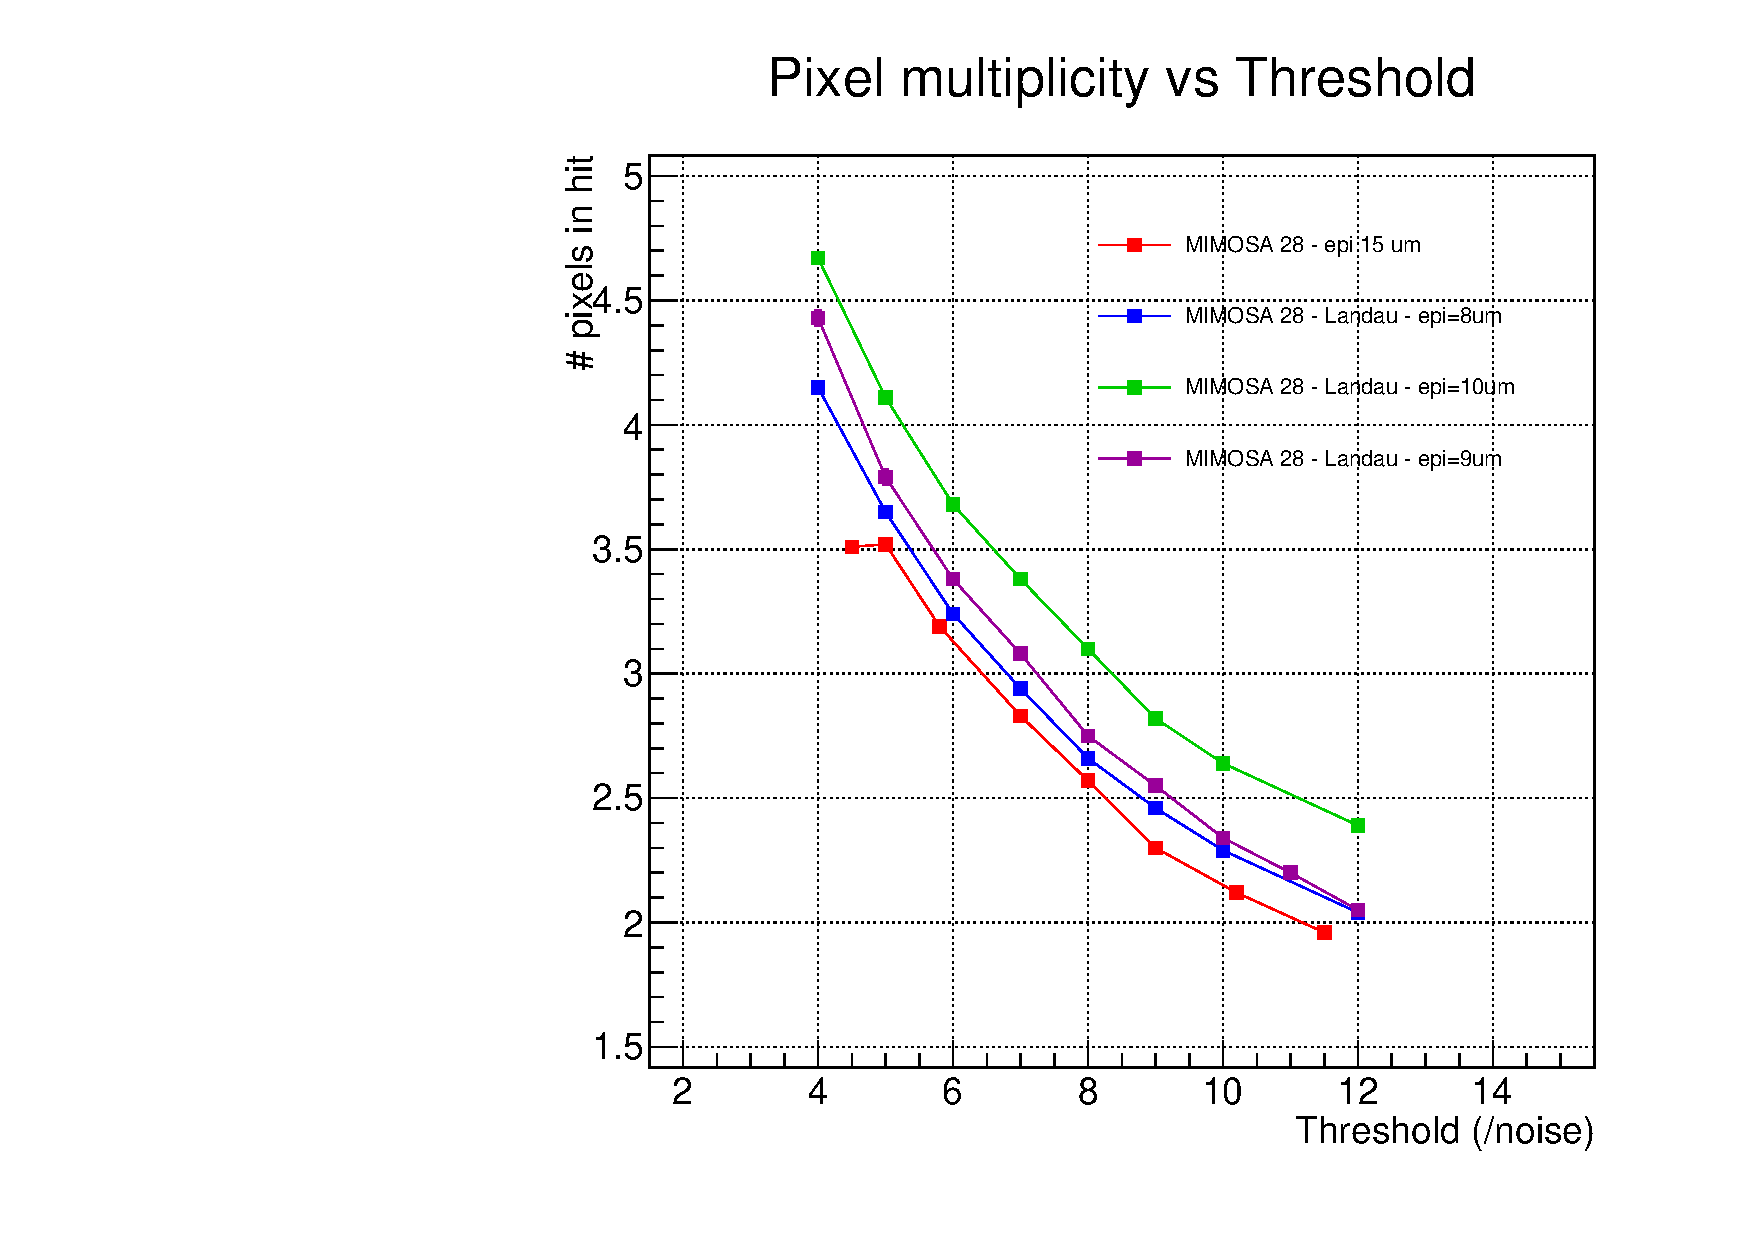
\includegraphics[scale=0.49]{./figures/Plots_resultat_simu/G4_landau_comparison_mult.pdf}
     \caption{Comparaison de la multiplicit\'e obtenue, pour diff\'erentes couches épitaxiées effectives, en fonction du seuil donn\'e en multiple du bruit moyen.}
     \label{fig:comp_landau_mult}
   \end{center}
   \end{figure}
   
   \medskip
   
   La figure \ref{fig:comp_landau_mult} expose la multiplicit\'e moyenne des amas de pixels, pour les diff\'erentes \'epaisseurs de couches épitaxiées effectives, en fonction du seuil en multiple du bruit moyen. Le tout est compar\'e \`a la multiplicit\'e moyenne des amas, d\'etermin\'ee en tests en faisceau, pour le capteur MIMOSA-28 HR15. Plus l'\'epaisseur de la couche épitaxiée est grande, plus la multiplicit\'e moyenne des amas augmente. Cela s'explique par l'augmentation du d\'ep\^ot de charge et par l'\'etalement plus important des charges dans la couche \'epitaxi\'ee lorsque celle-ci augmente. La multiplicit\'e moyenne est sup\'erieure au capteur de r\'ef\'erence pour toutes les \'epaisseurs de couches épitaxiées. Pour une couche épitaxiée \'epaisse de 10 $\mu m$ la multiplicit\'e moyenne varie entre 2.9 (12 $\sigma$) et 4.7 pixels par amas (4 $\sigma$). Lorsque la couche épitaxiée est \'epaisse de 9 $\mu m$, la multiplicit\'e varie entre 2.0 (12 $\sigma$) et 4.4 (4 $\sigma$) pixels par amas. Pour une couche épitaxiée de 8 $\mu m$, la multiplicit\'e varie entre 2.0 (12 $\sigma$) et 4.2 (4 $\sigma$) pixels par amas. A 7 $\sigma$ la multiplicit\'e est sup\'erieure d'environ $4 \%$, $9 \%$ et $19.5 \%$ pour des couches épitaxiées \'epaisses de respectivement 8, 9 et 10 $\mu m$. Pour une couche épitaxiée de 10 $\mu m$ l'\'ecart trop important en terme de multiplicit\'e moyenne des amas nous permet d'\'eliminer le choix d'une telle \'epaisseur.

  \medskip
   
   \begin{figure}[!htb]
    \begin{center} 
     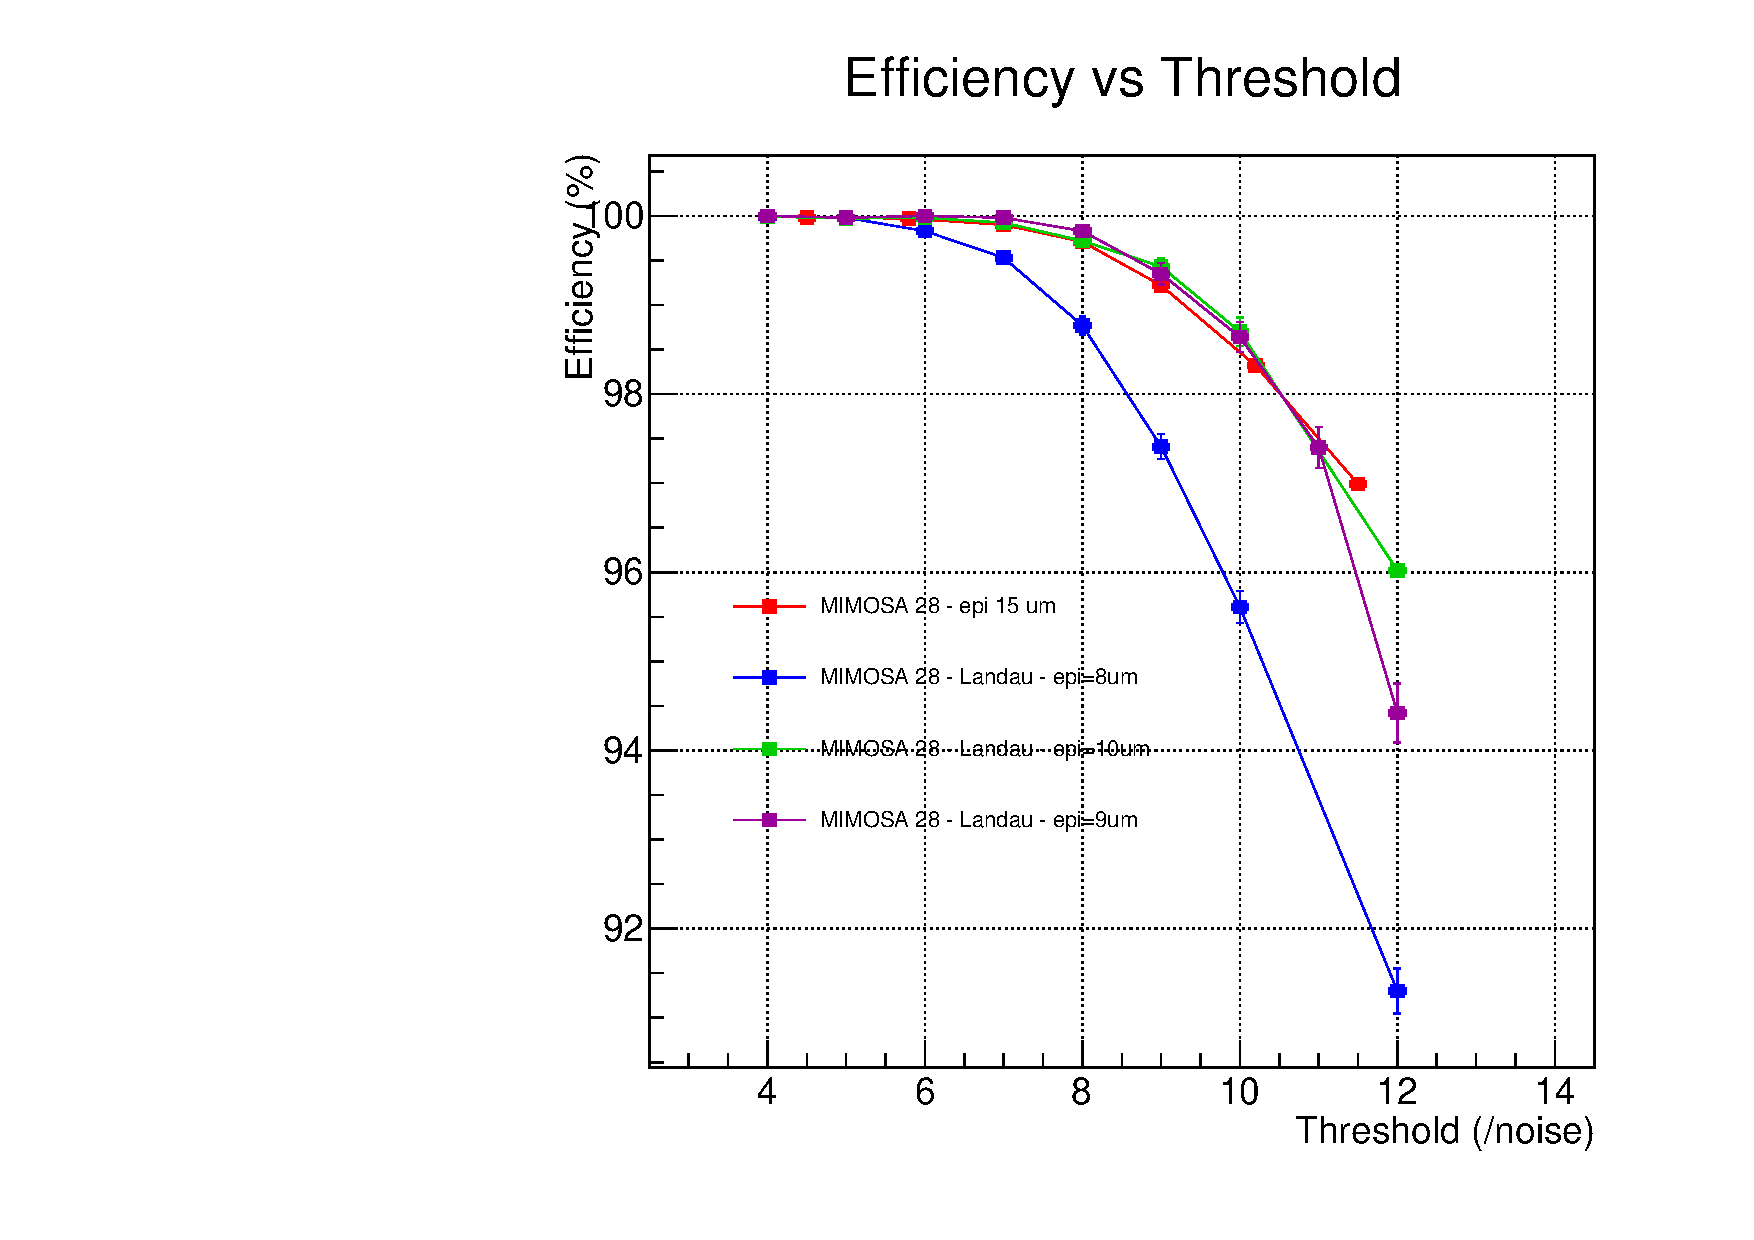
\includegraphics[scale=0.49]{./figures/Plots_resultat_simu/G4_landau_comparison_eff.pdf}
     \caption{Comparaison de l'efficacit\'e obtenue, pour diff\'erentes couches épitaxiées effectives, en fonction du seuil donn\'e en multiple du bruit moyen.}
     \label{fig:comp_landau_eff}
    \end{center}
   \end{figure}
   
   La figure \ref{fig:comp_landau_eff} donne l'efficacit\'e de d\'etection, obtenue pour les diff\'erentes \'epaisseurs de couches épitaxiées effectives, en fonction du seuil en multiple du bruit moyen. Le tout est compar\'e au capteur de r\'ef\'erence MIMOSA-28 HR15. 
   
   \medskip
   
   Voyons comment devrait se comporter l'efficacit\'e de d\'etection en fonction de l'\'epaisseur de la couche \'epitaxi\'ee. Premi\`erement on sait que plus la couche \'epitaxi\'ee est \'epaisse, plus la charge totale d\'epos\'ee est importante. Or plus la quantit\'e de charge d\'epos\'ee est importante, plus la charge collect\'e au niveau des pixels sera importante (dans la limite des faibles \'epaisseurs travers\'ees). Ainsi, plus la couche \'epitaxi\'ee est \'epaisse, plus la charge d\'epos\'ee est importante, plus le nombre de charges collect\'ees au niveau des pixels est important. Ainsi, plus la couche \'epitaxi\'ee est \'epaisse, plus le seuil du discriminateur d'au moins un pixel est souvent franchi. L'efficacit\'e devient alors de plus en plus importante lorsque la couche \'epitaxi\'ee s'\'epaissit (jusqu'\`a une certaine limite d'\'epaisseur).
   
   \medskip
   
   Comme attendu, plus l'\'epaisseur de la couche épitaxiée est grande plus l'efficacit\'e de d\'etection est importante.  Les valeurs de l'efficacité pour des \'epaisseurs de couches épitaxiées de 8 et 9 $\mu m$ collent aux donn\'ees jusqu'au seuil de 11 $\sigma$. Aux valeurs de coupure plus \'elev\'ees les donn\'ees des tests en faisceau ont une meilleure efficacit\'e de d\'etection. Pour une couche épitaxiée de 8 $\mu m$ l'efficacit\'e obtenue coïncide avec les donn\'ees jusqu'au seuil de 5 $\sigma$ puis l'\'ecart se creuse au dessus de ce seuil. On notera que pour des couches épitaxiées de 9 et 10 $\mu m$ une efficacit\'e sup\'erieure \`a 99.8 $\%$ est atteinte jusqu'au seuil de 8 $\sigma$ en tr\`es bon accord avec les donn\'ees des tests en faisceau. La faible efficacit\'e au dessus de 5 $\sigma$ pour une couche épitaxiée \'epaisse de 8 $\mu m$ permet d'\'eliminer le choix de cette \'epaisseur.

   \begin{figure}[!htb]
    \begin{center} 
     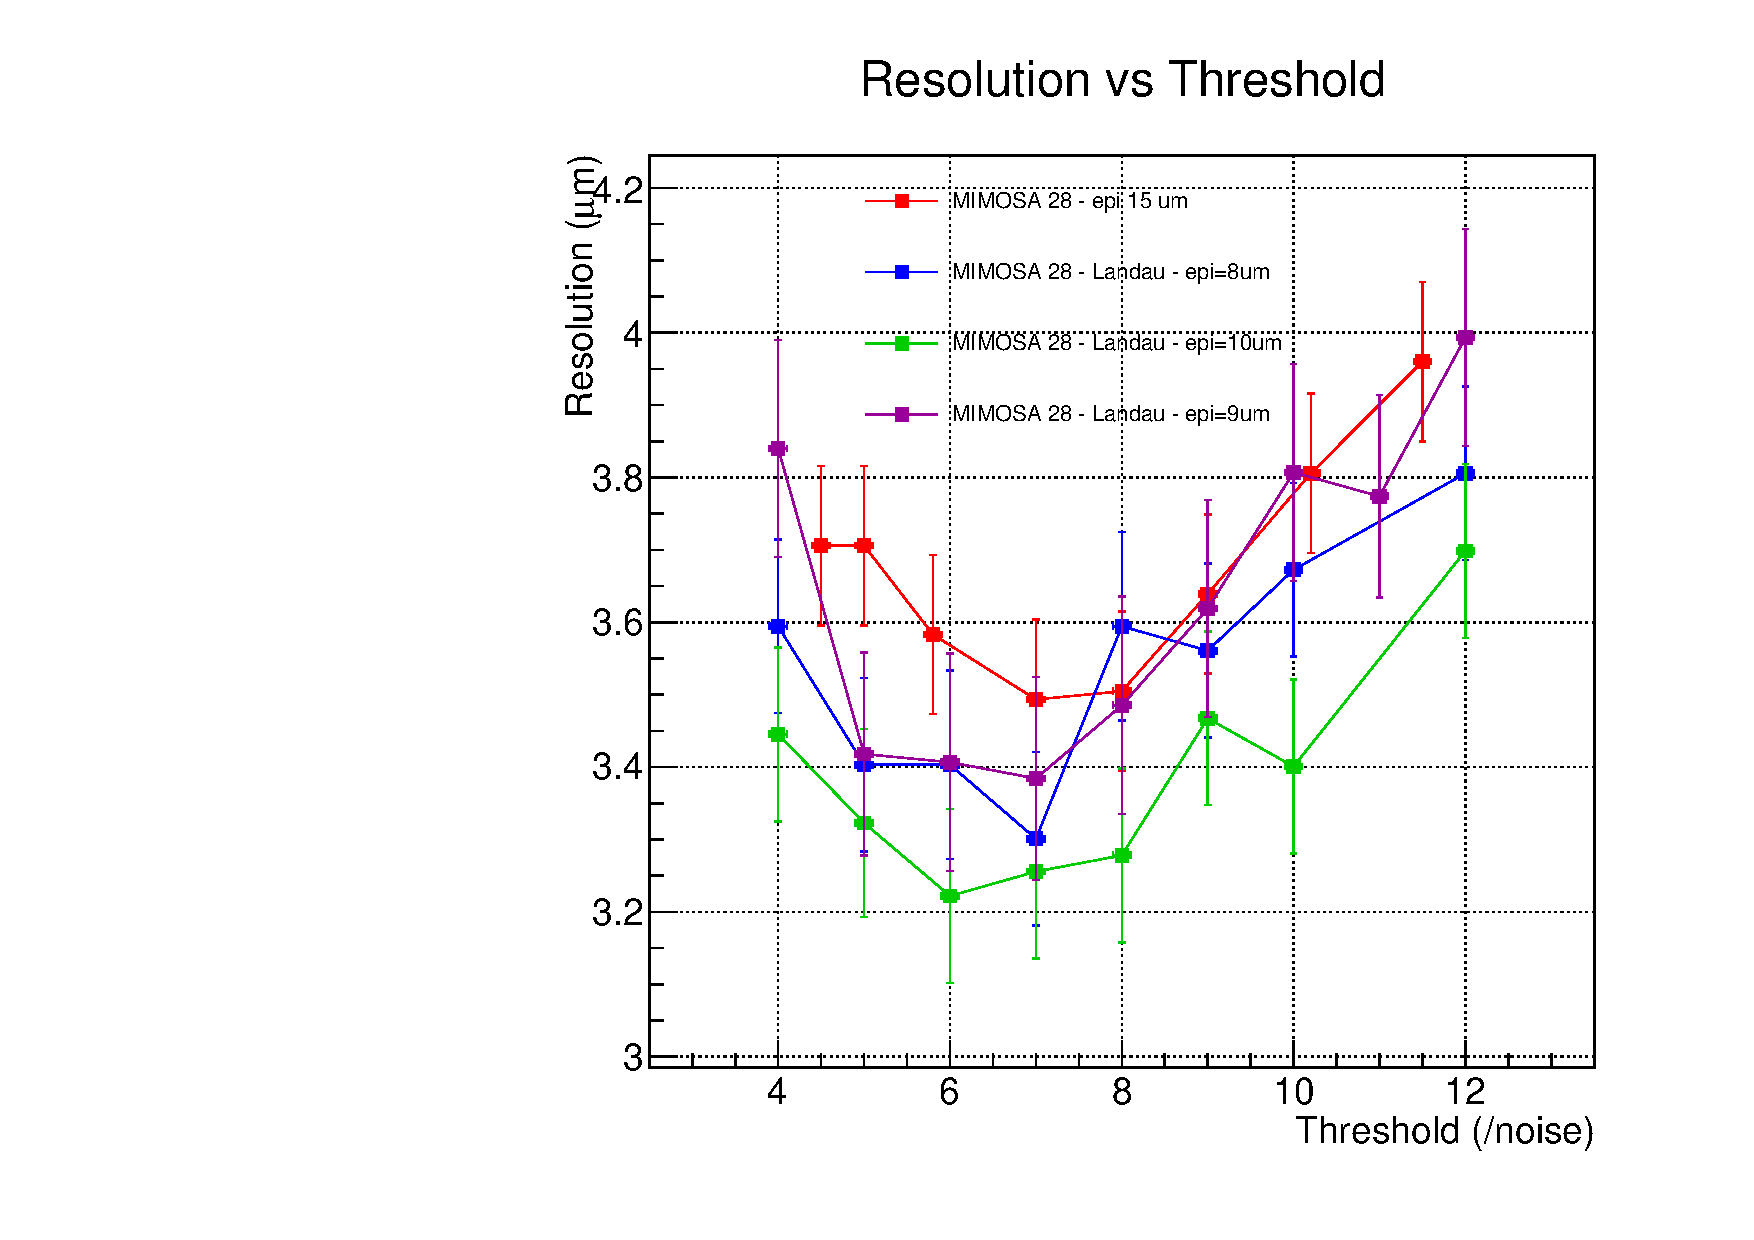
\includegraphics[scale=0.49]{./figures/Plots_resultat_simu/G4_landau_comparison_res.pdf}
     \caption{Comparaison de la r\'esolution spatiale obtenue, pour diff\'erentes couches épitaxiées effectives, en fonction du seuil donn\'e en multiple du bruit moyen.}
     \label{fig:comp_landau_res}
   \end{center}
   \end{figure} 
  
  \medskip
  
   La figure ~\ref{fig:comp_landau_res} donne la r\'esolution spatiale, obtenue pour les diff\'erentes \'epaisseurs de couche épitaxiée effective, en fonction du seuil en multiple du bruit moyen, compar\'ee au capteur de r\'ef\'erence MIMOSA-28 HR15. Pour une couche épitaxiée effective de 10 $\mu m$, la résolution spatiale obtenue varie dans un premier temps entre 3.45 (4 $\sigma$) et 3.25 (6 $\sigma$) $\mu m$. Puis celle-ci remonte jusqu'\`a atteindre la valeur de 3.7 $\mu m$ (12 $\sigma$). La r\'esolution spatiale obtenue est inf\'erieure \`a celle du capteur de r\'ef\'erence d'environ 0.2 \`a 0.4 $\mu m$. Pour les couches épitaxiées d'\'epaisseur 8 et 9 $\mu m$, la r\'esolution spatiale est en bon accord avec les donn\'ees, aux marges d'erreurs pr\`es, except\'e \`a 5 $\sigma$ ou elle est environ 0.3 $\mu m$ en dessous du capteur de r\'ef\'erence. Pour une \'epaisseur de couche épitaxiée de 9 $\mu m$, la r\'esolution spatiale diminue dans un premier temps en passant de environ 3.85 (4 $\sigma$) \`a 3.4 (7 $\sigma$) $\mu m$ puis remonte jusqu'\`a atteindre la valeur de 4 $\mu m$ (12 $\sigma$). Quant aux valeurs de r\'esolution spatiale pour une couche épitaxiée de 8 $\mu m$, elle passe de 3.6 \`a 3.3 $\mu m$ entre 4 et 7 $\sigma$  puis remonte jusqu'a 3.8 $\mu m$ \`a 12 $\sigma$. On notera que malgr\'e une multiplicit\'e des amas plus importante, la r\'esolution spatiale pour une couche épitaxiée de 10 $\mu m$ est inf\'erieure \`a celle pour une \'epaisseur de couche épitaxiée de 8 et 9 $\mu m$. Cela peut s'expliquer par l'obtention d'un meilleur centre de gravit\'e avec des amas compos\'es de 4 pixels compar\'es \`a ceux compos\'es de 2 ou 3 pixels.
   
   \medskip

   \'A la vue de ces r\'esultats, l'\'epaisseur de couche épitaxiée choisie est de 9 $\mu m$. Il s'agit en effet du meilleur compromis en terme de multiplicit\'e des amas, d'efficacit\'e et de r\'esolution spatiale. Nous utiliserons donc ce mod\`ele de d\'epôt de charges pour nos simulations.
   
%Comparaison avec les donn\'ees r\'eelles \\
%Plots caract\'eristiques simu vs capteurs reel. \\
%Comparaison avec les donn\'ees des tests faisceau \\
%Expliquer les differences. \\
   
   \medskip
   
   Afin de tester notre simulation nous allons caract\'eriser les propri\'et\'es de nos capteurs et de nos \'echelles en fonction de leurs inclinaisons.
   
   \FloatBarrier
   
   %Nous examinerons aussi la variation de la largeur de distribution des r\'esidus pour un syst\`eme d'\'echelles doubles faces distantes d'une longueur variable.
  
   \subsection{Exploration des propri\'et\'es des capteurs simul\'es}

   Nous allons dans un premier temps \'etudier l'influence de l'inclinaison du \textit{DUT} sur les param\`etres du capteur simul\'e \'etudi\'e. Cela correspond aussi \`a des traces d'incidence non normales. On notera que notre m\'ethode de mise en amas n'a pas \'et\'e \'etudi\'ee sp\'ecifiquement pour les incidences non normales. Cependant, nous verrons que pour ces incidences non-normales, notre m\'ethode de mise en amas reste encore valide.
%Puis nous examinerons quelques propri\'et\'es des \'echelles PLUME en d\'ecrivant l'\'evolution de la distribution des r\'esidus sur les deux faces d'une \'echelle PLUME en fonction de la distance entre deux \'echelles PLUME et en fonction de l'impulsion du faisceau de particules
%  \`a une distance fix\'ee.
   
   \FloatBarrier
   
   \subsubsection{G\'eom\'etrie}
 
   \begin{figure}[!hbt]
    \begin{center} 
     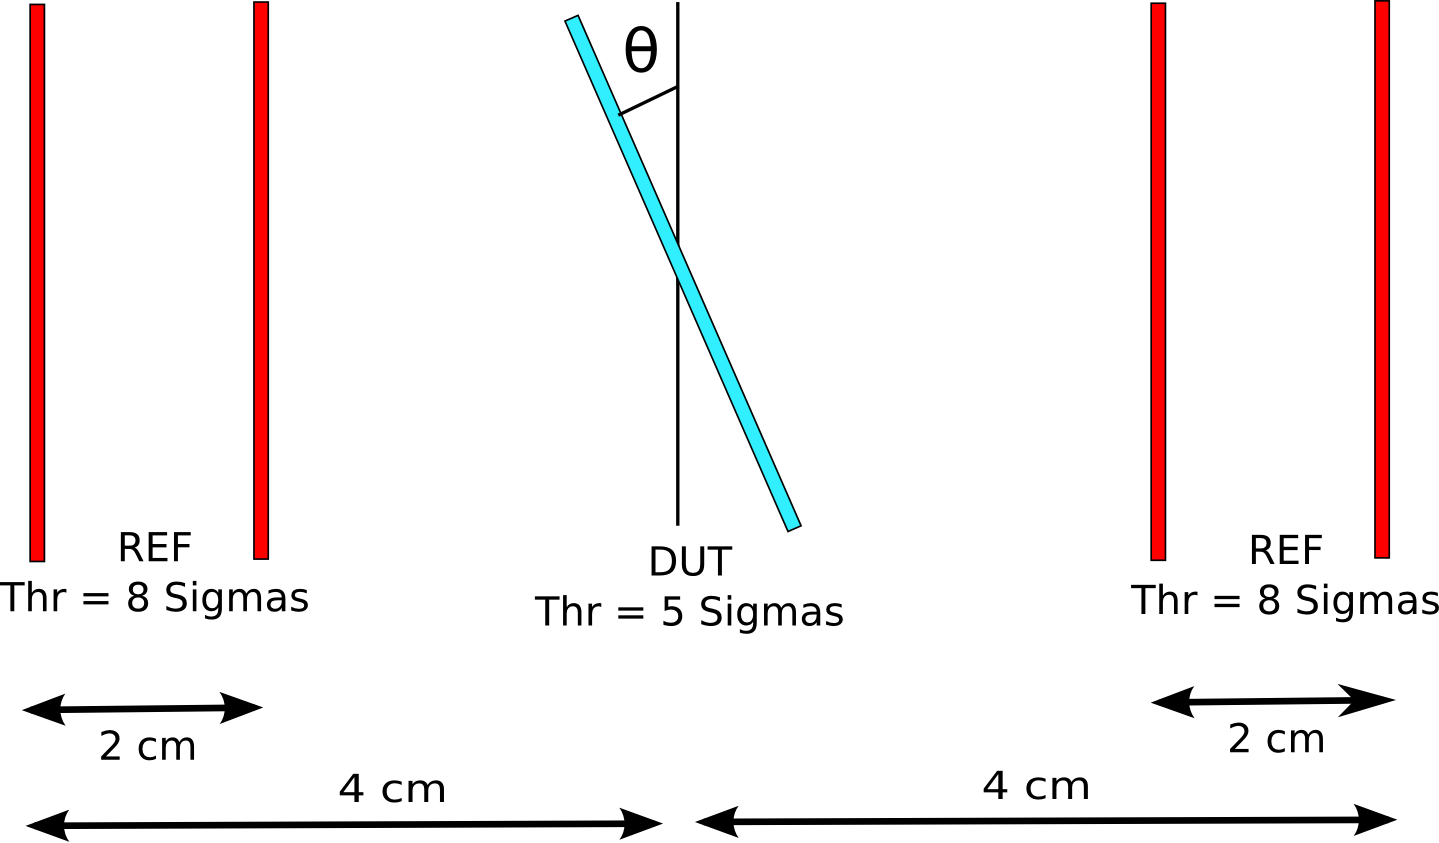
\includegraphics[scale=0.75]{./figures/config_5_plane_DUT_tilt.png}
     \caption{G\'eom\'etrie du t\'elescope. Vue de cot\'e : dans le plan $yOz$. En rouge les quatre plans de r\'ef\'erences et en bleu le \textit{DUT} inclin\'e d'un angle $\theta$ selon l'axe $Ox$}
    \label{fig:tel_tilt}
    \end{center}
   \end{figure} 
   
   La figure \ref{fig:tel_tilt} illustre la g\'eom\'etrie du t\'elescope utilis\'ee pour nos \'etudes avec inclinaison du DUT. Le t\'elescope est compos\'e de 4 plans de r\'ef\'erences MIMOSA-28 HR15 simul\'es avec un seuil des discriminateurs fix\'e \`a 8 fois la valeur moyenne du bruit moyen. Le \textit{DUT} de type MIMOSA-28 HR15 utilise quant \`a lui un seuil des discriminateurs de 5 fois le bruit moyen et est inclin\'e d'un angle $\theta$ par rapport à l'axe $Ox$. Tous les plans sont espac\'es de 2 $cm$ entre eux selon l'axe $Oz$. Les particules utilis\'ees sont des pions n\'egatifs dot\'es d'une impulsion de 120 $GeV/c$. Ceux-ci sont envoy\'es parall\`element \`a l'axe $Oz$ du t\'elescope. Les traces sont reconstruites \`a partir des quatre plans de r\'ef\'erence.
   
   \subsubsection{Multiplicit\'e en fonction de l'inclinaison du capteur}
   
   La figure \ref{fig:mult_vs_tilt} repr\'esente la multiplicit\'e des amas de pixels en fonction de l'inclinaison du capteur selon l'axe $Ox$. Cela peut aussi \^etre vu comme des traces poss\'edant un angle d'incidence $\theta$ par rapport \`a la normale. La figure \ref{fig:mult_vs_tilt} indique que la multiplicit\'e augmente en fonction de l'angle. Nous pouvons cr\'eer un mod\`ele simple pour la variation de multiplicit\'e en fonction de l'angle $\theta$ d'incidence des traces. Le rapport entre la longueur travers\'ee dans la couche \'epitaxi\'ee par des traces \`a incidence normale par rapport \`a des traces d'angle d'incidence $\theta$ vaut :
   
   \begin{equation}
    \cfrac{L_{epi}^{\theta=0}}{L_{epi}^{\theta}} = \cfrac{1}{\cos(\theta)}
   \end{equation}
   
   Ce rapport correspond aussi au rapport des charges d\'epos\'ees dans la couche \'epitaxi\'ee en fonction de l'angle d'incidence des traces. Une modélisation pour la multiplicit\'e $M(\theta)$ en fonction de $\theta$ peut ainsi \^etre la suivante :
   
%    En distinguant deux axes pour les amas \`a incidence non normale, l'un selon l'entendu de l'amas (selon le parcourt de la trace \`a incidence non normale) et l'autre selon la largeur de l'amas, on peut estimer la multiplicit\'e de l'amas en utilisant deux termes. Le premier terme, repr\'esente la largeur moyenne de l'amas \`a incidence moyenne et vaut environ $\cfrac{M(\theta=0)}{2}$. Le second terme représente l'\'etendu de l'amas et vaut $\cfrac{1}{\cos(\theta)}$ fois la largeur moyenne de l'amas \`a incidence non normale. On peut alors mod\'eliser la multiplicit\'e $M(\theta)$ en fonction de $\theta$ comme :
   
   \begin{equation}
    M(\theta) = \cfrac{M(\theta=0)}{2} \left( 1 + \cfrac{1}{\cos(\theta)} \right)
   \end{equation}

   Avec $M(\theta=0) = 3.80$ la multiplicit\'e \`a incidence normale. Sur la figure \ref{fig:mult_vs_tilt}, ce mod\`ele est superpos\'e aux valeurs mesur\'ees pour diff\'erentes inclinaisons. Il d\'ecrit assez bien l'\'evolution de la multiplicit\'e en fonction de l'inclinaison du capteur.
   
   \begin{figure}[!Htb]
    \begin{center} 
     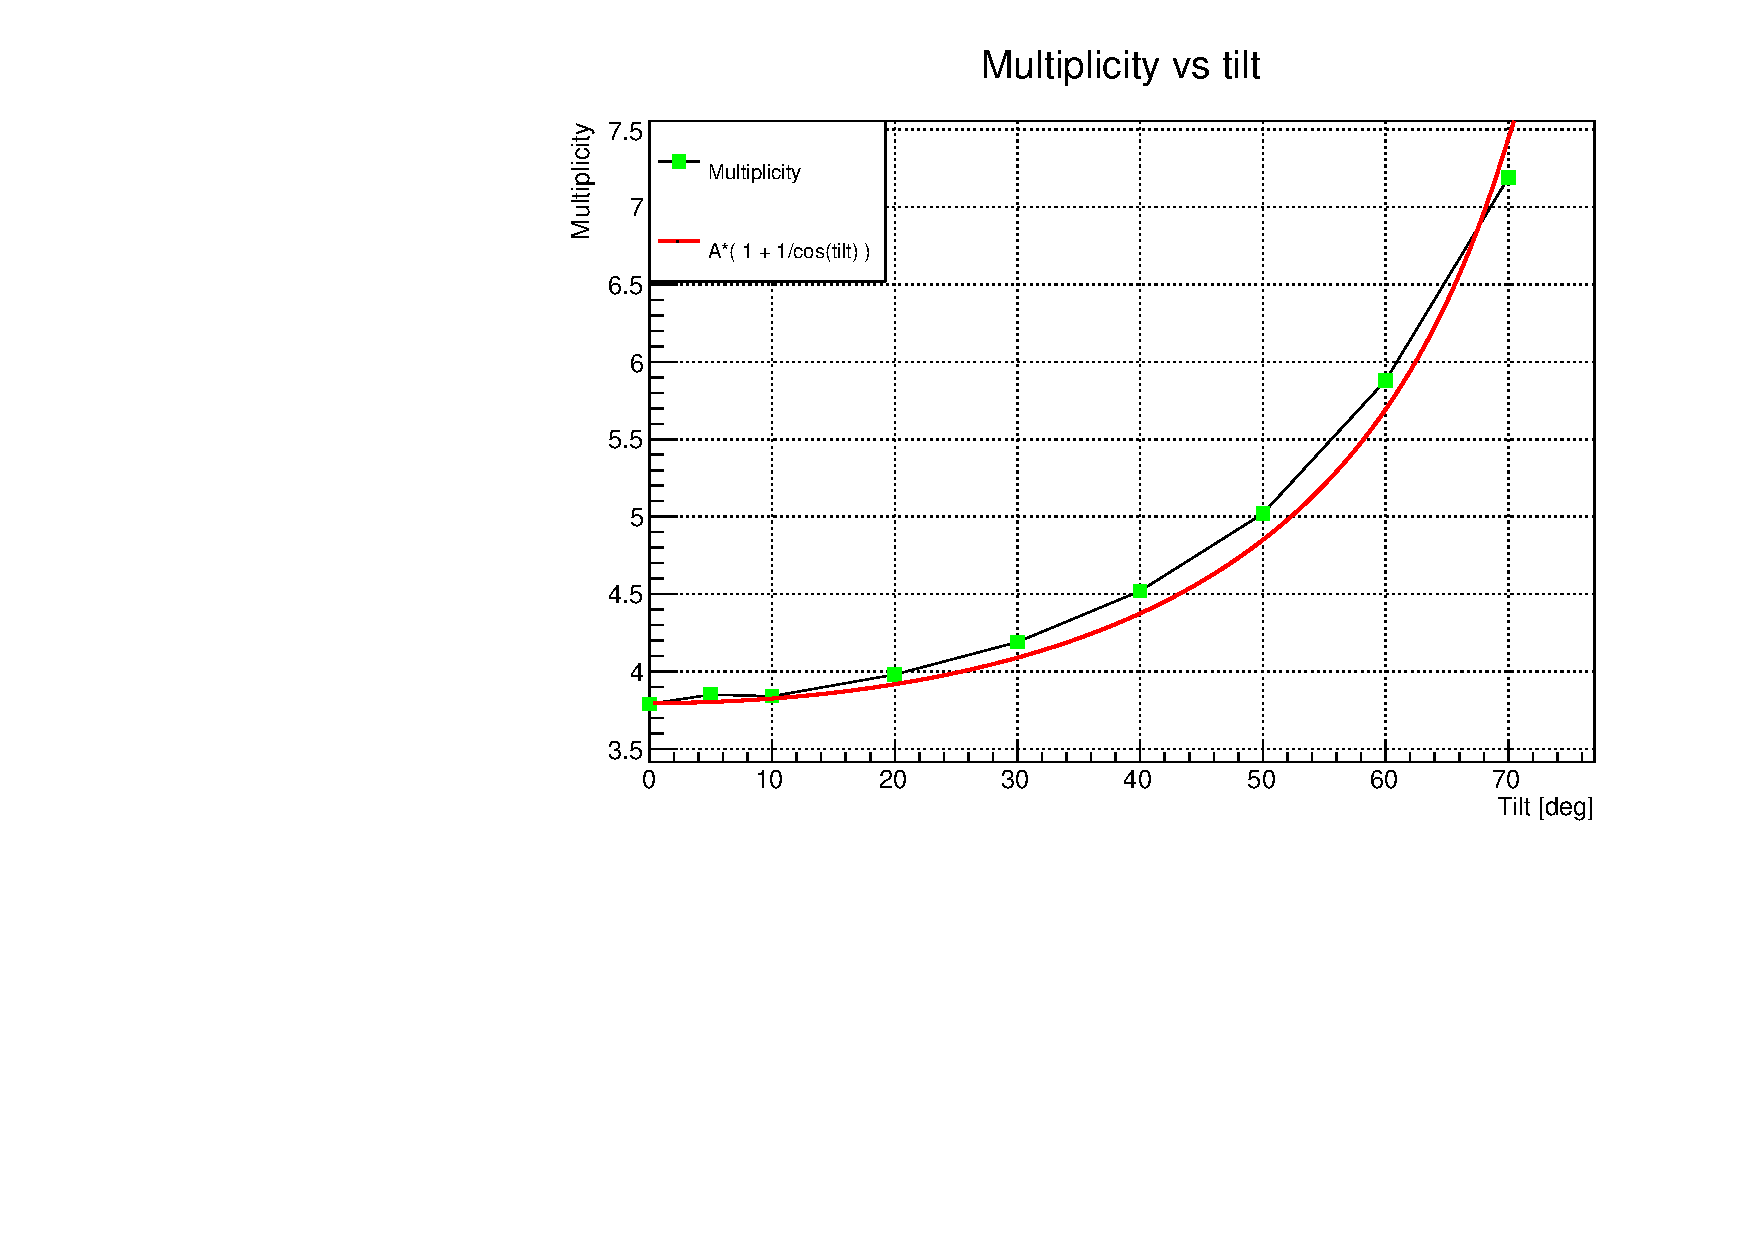
\includegraphics[scale=0.65]{./figures/multiplicity_vs_tilt.pdf}
     \caption{En vert, multiplicit\'e en fonction de l'inclinaison du capteur selon son axe Oy. En rouge, mod\`ele simple de variation de la multiplicit\'e.}
    \label{fig:mult_vs_tilt}
    \end{center}
   \end{figure}
   
   \FloatBarrier
   
   \subsubsection{\ Efficacit\'e de d\'etection en fonction de l'inclinaison du capteur}

%    La figure \ref{fig:effi_vs_tilt} illustre l'efficacit\'e de d\'etection des particules passant \`a travers le capteur en fonction de l'inclinaison de ce dernier. 
   
   L'efficacit\'e reste constante et sup\'erieure \`a $99.9\%$ pour un seuil appliqu\'e aux discriminateurs de 5 fois le bruit moyen quelque soit l'inclinaison du capteur entre 0 et $70$ degr\'es. Ce r\'esultat \'etait attendu puisque le d\'epôt de charge est plus \'elev\'e lorsque la trace poss\`ede un angle $\theta$ d'incidence non nul. La trace parcourt en effet un chemin $\cfrac{1}{cos(\theta)}$ plus important dans la couche \'epitaxi\'ee.
   
%    \begin{figure}[!Htb]
%     \begin{center} 
%      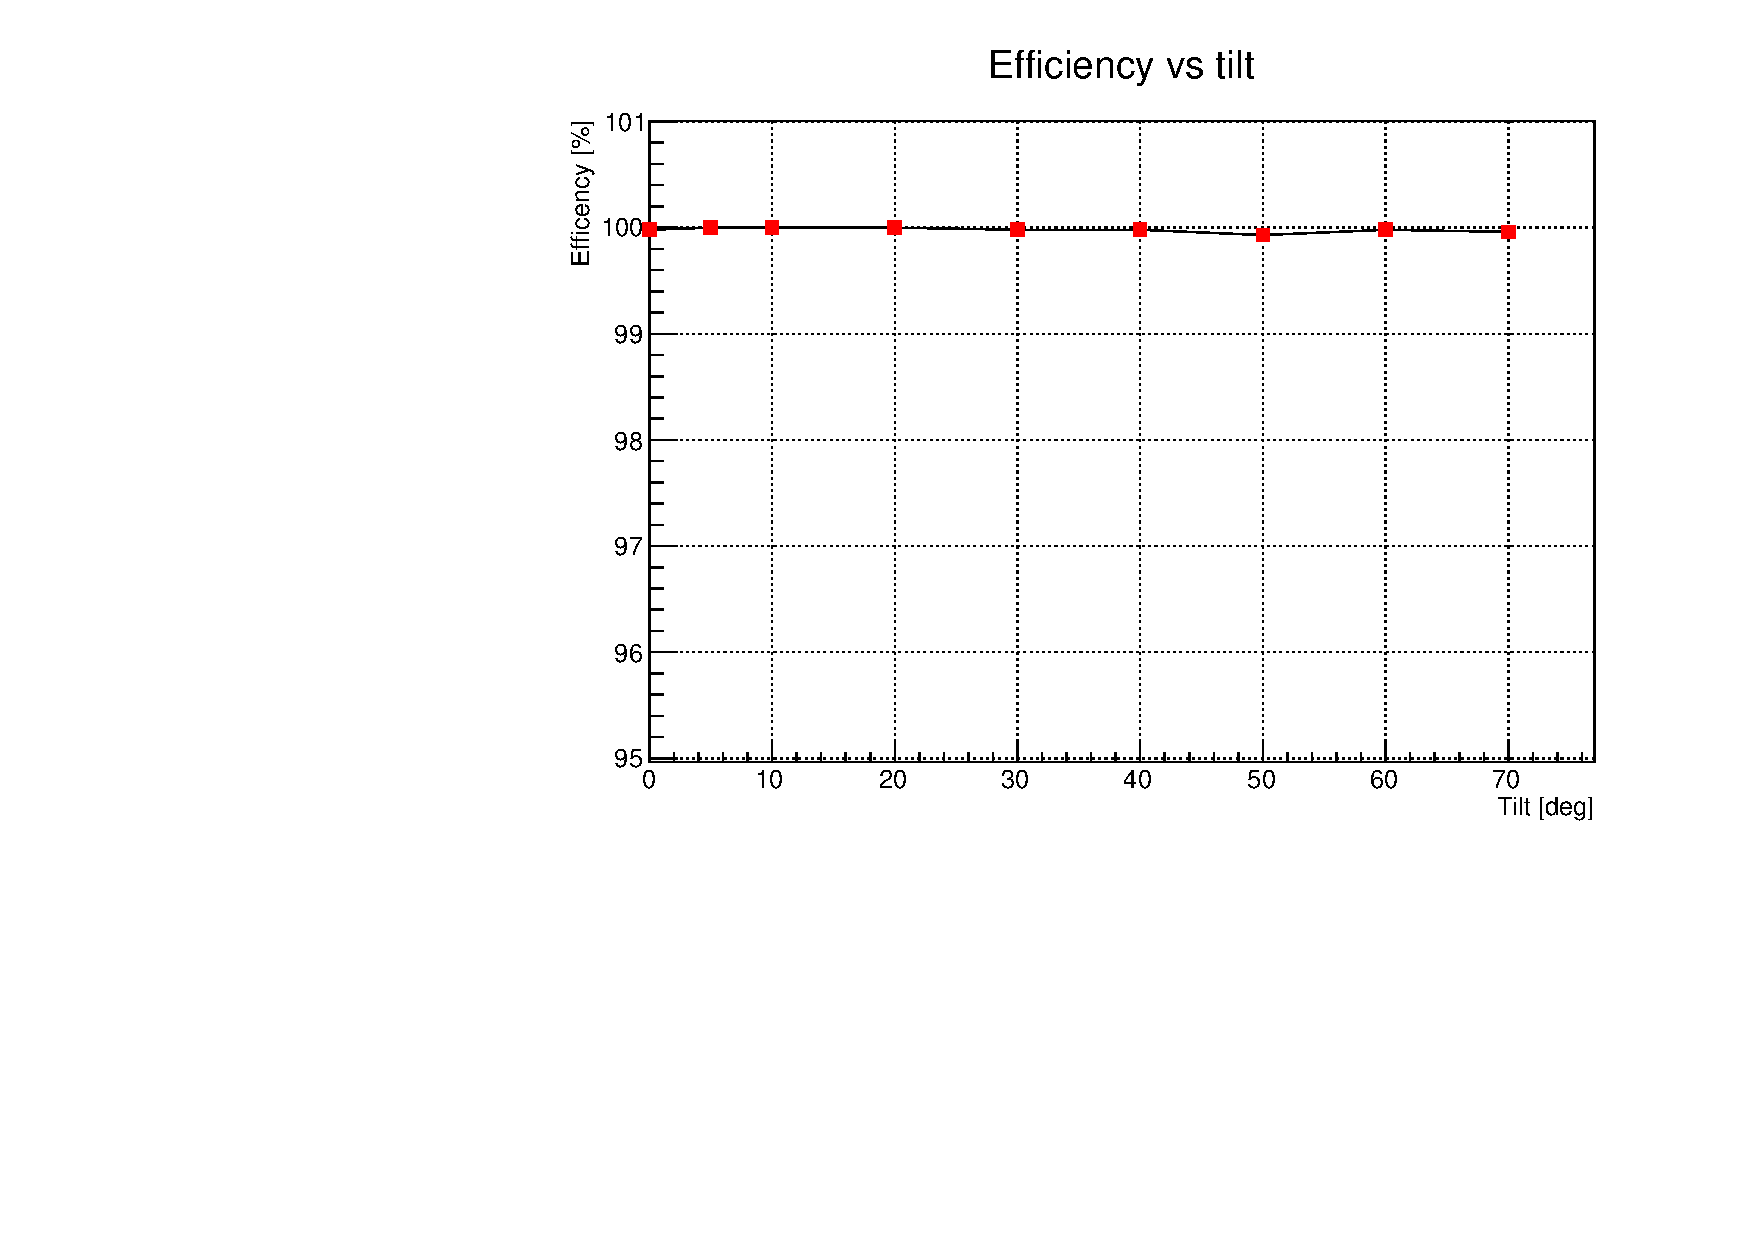
\includegraphics[scale=0.80]{./figures/efficiency_vs_tilt.pdf}
%      \caption{Efficacit\'e de d\'etection en fonction de l'inclinaison du capteur.}
%     \label{fig:effi_vs_tilt}
%     \end{center}
%    \end{figure}   

   \subsubsection{R\'esolution en fonction de l'inclinaison du capteur}
   
   La figure \ref{fig:reso_vs_tilt} illustre la variation de la r\'esolution spatiale du DUT en fonction de son inclinaison. Rappelons que celle-ci est \'egale \`a la racine de la soustraction quadratique de la largeur de la distribution des r\'esidus avec la r\'esolution du t\'elescope et la diffusion multiple selon l'\'equation \ref{eq:resolution}. Nous considérerons la diffusion multiple nulle \'etant donn\'ee l'impulsion des pions valant 120 $GeV/c$. Étant donn\'e l'inclinaison du capteur, la r\'esolution spatiale du t\'elescope varie l\'eg\`erement si l'on se trouve au bord du capteur ou au centre de celui-ci. La position $z$ n'est en effet pas la m\^eme. Selon la composition et la configuration du t\'elescope, la r\'esolution du t\'elescope vaut $1.75 \, \mu m$ au centre du \textit{DUT}. Dans le cas extr\^eme ou le \textit{DUT} est inclin\'e de 70 degr\'es, la r\'esolution du t\'elescope sur un des bords de ce dernier vaut $1.88 \, \mu m$. On rappelle que dans notre configuration, la r\'esolution spatiale est sym\'etrique par rapport \`a $z=0$. Cet effet n'a pas \'et\'e consid\'er\'e dans le calcul de la r\'esolution du DUT, et la valeur constante de $1.75 \, \mu m$ pour la r\'esolution t\'elescope a \'et\'e utilis\'ee. Nous allons expliciter les raisons de cette approximation.
   
  \begin{figure}[!Htb]
    \begin{center} 
     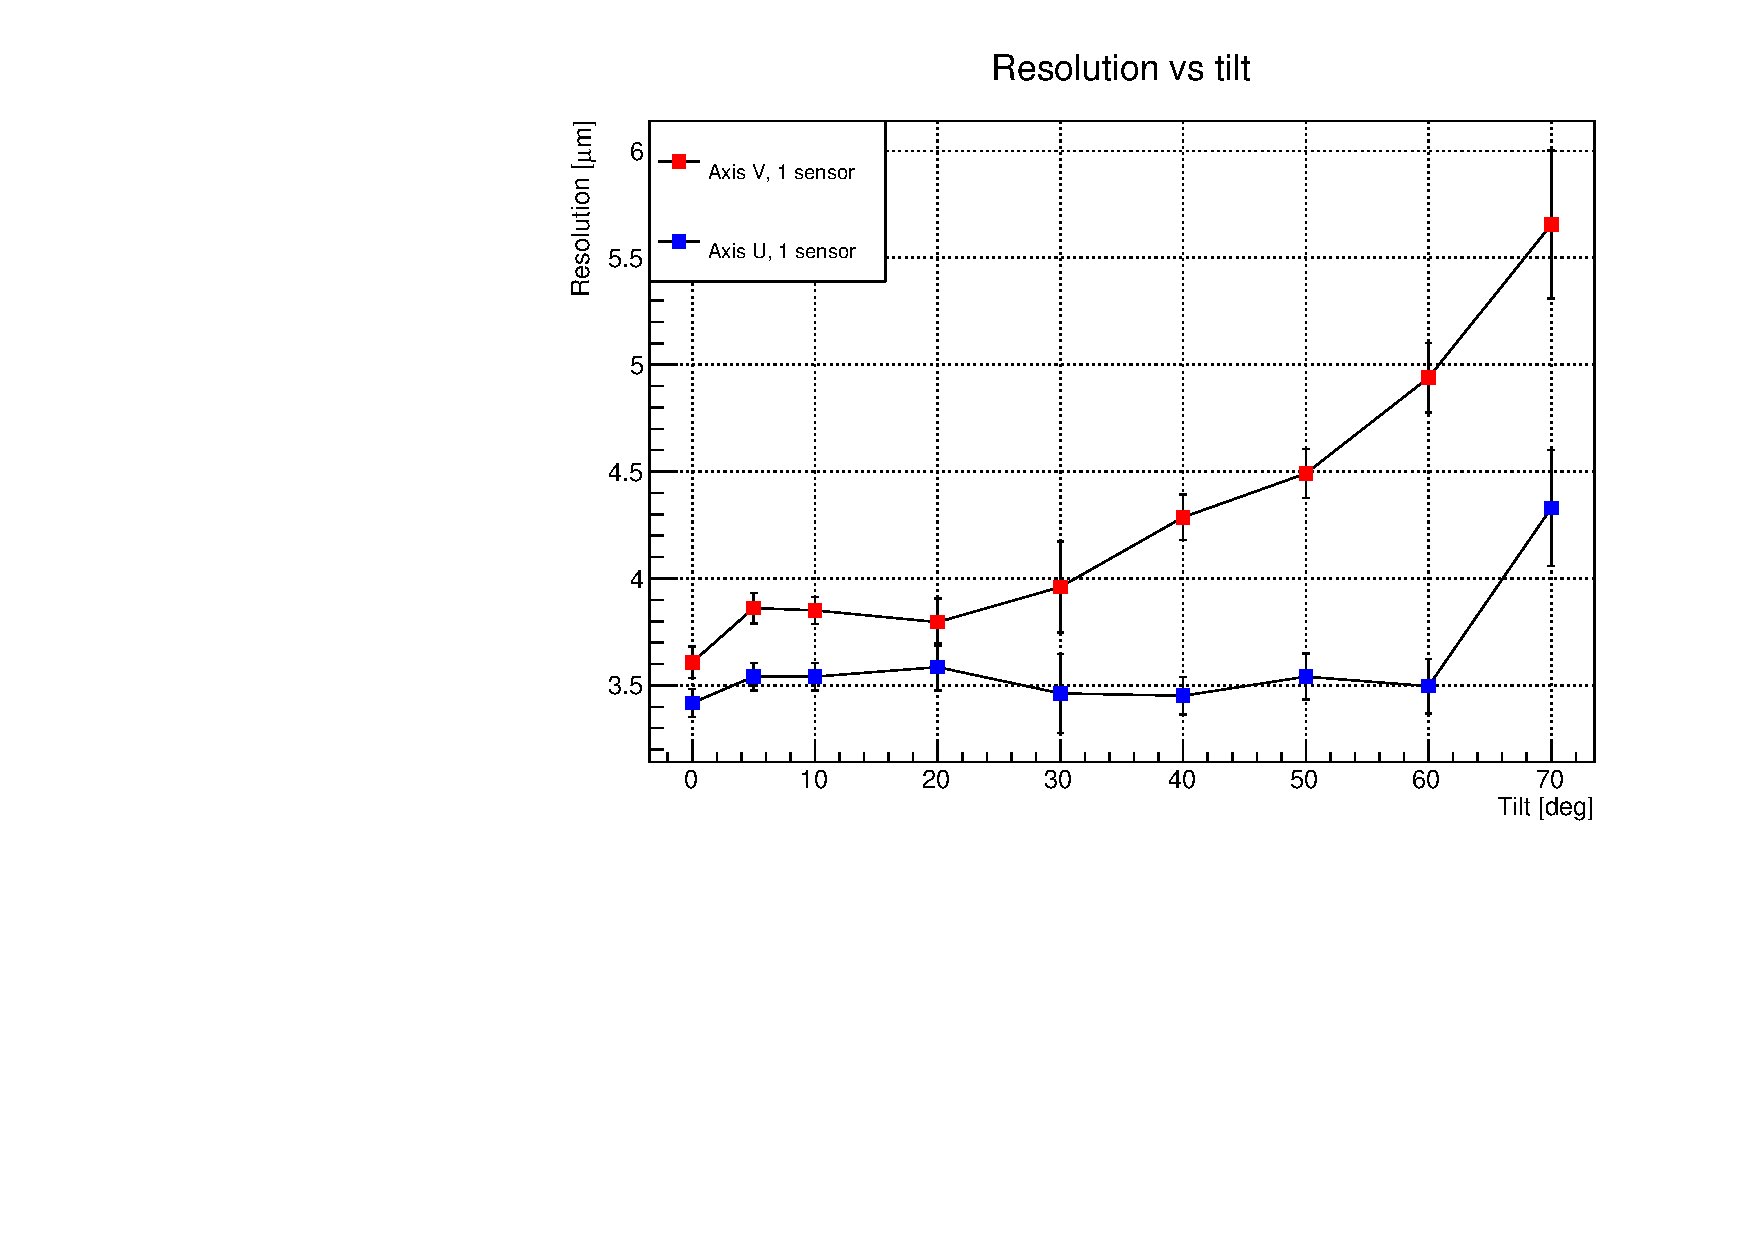
\includegraphics[scale=0.65]{./figures/reso_vs_tilt_1_sensor.pdf}
     \caption{R\'esolution en fonction de l'inclinaison du capteur selon son axe Ox.}
    \label{fig:reso_vs_tilt}
    \end{center}
  \end{figure}
   
   \medskip
   
   Nous allons alors estimer l'erreur commise. Pour cela, on calcule selon l'\'equation \ref{reso_tel_4_plans} et selon l'inclinaison du \textit{DUT} la valeur de la r\'esolution du t\'elescope en fonction de la longueur du \textit{DUT}. Quelques unes de ces valeurs ont \'et\'e calcul\'ees pour une inclinaison de $70$ degr\'es du \textit{DUT}. Elles sont pr\'esent\'ees sur la figure \ref{fig:res_tel_vs_tilt}. Cette figure repr\'esente la valeur de la r\'esolution du t\'elescope en fonction de la distance $l$ de l'impact selon l'axe V du capteur par rapport \`a une origine prise sur le bord inf\'erieur ou sup\'erieur du capteur, divis\'ee par la longueur totale $L$ du \textit{DUT}. Dans notre configuration de t\'elescope, la résolution spatiale du t\'elescope selon l'axe $Oz$ \'evolue quadratiquement. Ainsi, le probl\`eme est sym\'etrique. L'origine $l=0$ peut donc \^etre prise sur le bord inf\'erieur ou sup\'erieur du DUT.
   
  \begin{figure}[!Htb]
    \begin{center} 
     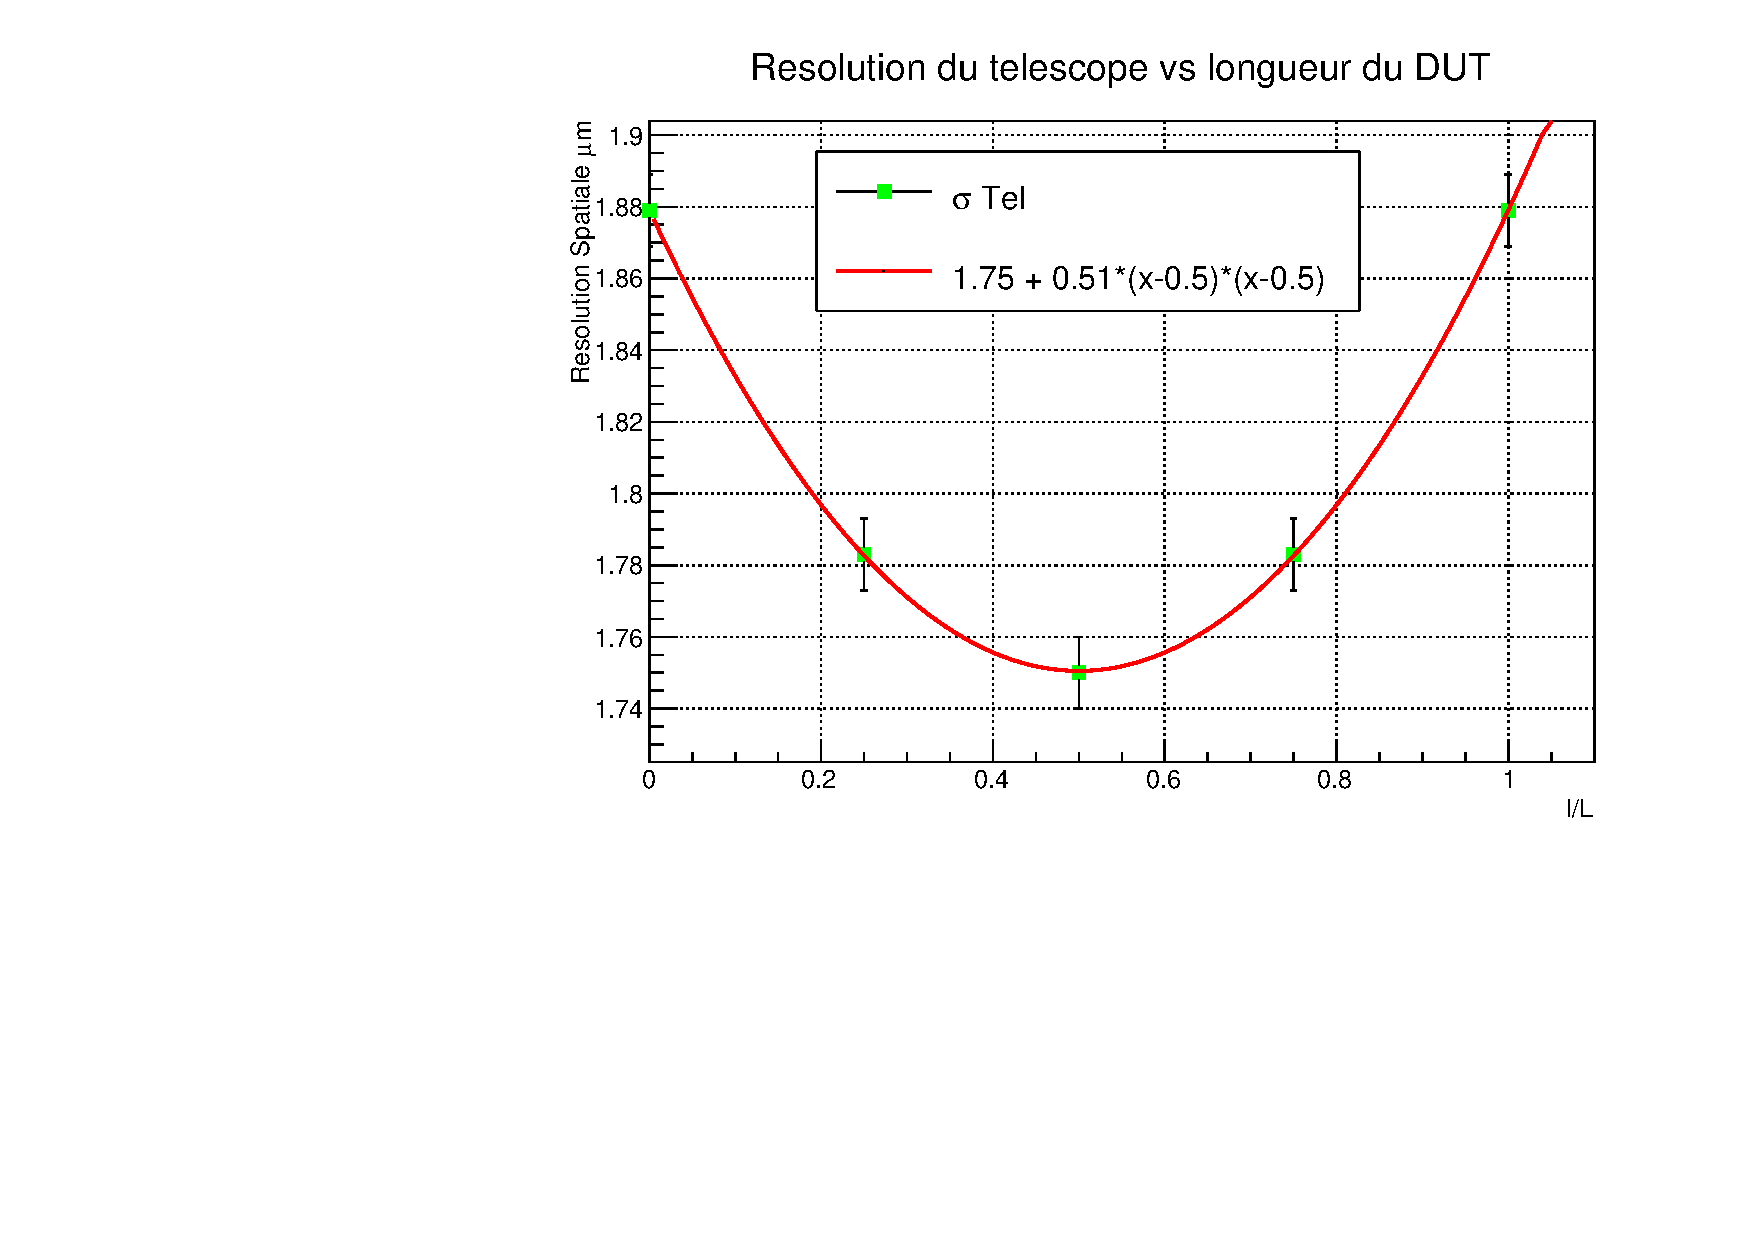
\includegraphics[scale=0.65]{./figures/Res_tel_tilt_DUT.pdf}
     \caption{R\'esolution du t\'elescope en fonction de la position U du DUT.}
    \label{fig:res_tel_vs_tilt}
    \end{center}
   \end{figure}
   
   \medskip
   
   Un mod\`ele quadratique en $x = l/L$ a ensuite \'et\'e ajust\'e pour rendre compte de la r\'esolution du t\'elescope en fonction de la position de l'impact d'une trace sur le \textit{DUT}. Ce mod\`ele est le suivant : 
   
   \begin{equation}
    \sigma_{tel}(x) = A + B (x-0.5)^2 
    \label{eq:modele}
   \end{equation}

   Les valeurs pour A et B sont les suivantes : $A =\sigma_{tel}(x=0.5) = 1.75$ et $B = 0.51$ (obtenues apr\`es ajustement). Supposons maintenant que les impacts sur le \textit{DUT} sont r\'epartis de fa\c{c}on homog\`ene, c'est-\`a-dire que la densit\'e d'impacts est la m\^eme sur toute la surface du \textit{DUT}. Il suffit alors d'int\'egrer l'\'equation \ref{eq:modele} entre 0 et 1 selon la variable x pour obtenir la r\'esolution moyenne du t\'elescope. Apr\`es calcul, la r\'esolution moyenne du t\'elescope pour un DUT inclin\'e \`a $70$ degr\'es vaut environ $\sigma_{tel} = 1.80 \, (1.7925)\, \mu m$. Il s'agit d'une valeur environ $2.5\%$ plus \'elev\'ee que la valeur de base $\sigma_{tel} = 1.75$. De plus, il s'agit de la valeur moyenne la plus \'elev\'ee puisque elle est calcul\'ee pour une inclinaison du \textit{DUT} maximale de $70$ degr\'es. \'Etant donn\'ees les erreurs sur la r\'esolution des plans de r\'ef\'erence du t\'elescope, la valeur de la r\'esolution du t\'elescope au niveau du centre du \textit{DUT} est aussi soumise \`a une erreur. Ainsi, nous consid\'erons la r\'esolution du t\'elescope constante et valant $1.75 \, \mu m$ et nous attribuerons une erreur de $0.1 \, \mu m$ sur cette r\'esolution. Pour effectuer les calculs de la r\'esolution spatiale du \textit{DUT} nous avons pris une r\'esolution spatiale du t\'elescope \'egale \`a $1.75 \pm 0.1 \, \mu m$ et une erreur statistique sur la largeur de la distribution des r\'esidus valant $\Delta \sigma_{res} = \sigma_{res}/\sqrt{N}$, avec $N$ le nombre de traces passant \`a travers le DUT. Les erreurs sont calcul\'ees selon la relation de propagation des erreurs suivantes :
   
   \begin{equation}
    \Delta \sigma_{DUT} = \sqrt{ \dfrac{\sigma_{res}^2}{\sigma_{res}^2 - \sigma_{tel}^2} (\Delta \sigma_{res})^2 + \dfrac{\sigma_{tel}^2}{\sigma_{res}^2 - \sigma_{tel}^2} (\Delta \sigma_{tel})^2 }
   \end{equation}
   
   Que l'on peut aussi \'ecrire : 
   
   \begin{equation}
    \Delta \sigma_{DUT} = \sqrt{ \dfrac{\sigma_{res}^2}{\sigma_{res}^2 - \sigma_{tel}^2} \dfrac{\sigma_{res}^2}{N} + \dfrac{\sigma_{tel}^2}{\sigma_{res}^2 - \sigma_{tel}^2} (\Delta \sigma_{tel})^2 }
   \end{equation}
   
   \medskip
   
   La figure \ref{fig:reso_vs_tilt} indique que la r\'esolution spatiale du \textit{DUT} en fonction de son inclinaison reste constante \`a environ $3.5 \, \mu m$ selon l'axe U du capteur (correspondant ici \`a l'axe Ox du t\'elescope) hormis pour le point \`a $70$ degr\'es ou elle atteint $4.3 \, \mu m$. Entre $0$ et $5$ degr\'es la r\'esolution spatiale du \textit{DUT} selon l'axe V du capteur augmente de $3.6 \, \mu m$ \`a $3.9 \, \mu m$ puis celle-ci reste stable jusqu'\`a $20$ degr\'es. Entre $20$ et $70$ degr\'es la r\'esolution spatiale du \textit{DUT} selon son axe V augmente de nouveau en passant de respectivement de $3.8 \, \mu m$ \`a $5.7 \, \mu m$.
   
   \medskip
   
   Ainsi, la r\'esolution spatiale selon l'axe horizontal $U$ du capteur reste identique lorsque le capteur est inclin\'e selon son axe horizontal $U$. De plus, selon l'axe vertical $V$ du capteur, la r\'esolution spatiale se d\'egrade au fur et \`a mesure que l'on incline le capteur selon son axe horizontal $U$. Cela s'explique par la plus grande longueur travers\'ee dans la couche \'epitaxiale selon l'axe $V$ du capteur. \`A haute impulsion, cette longueur travers\'ee vaut $L = \cfrac{ L_{epi} }{ \cos{\theta} }$. L'\'etendue \`a la surface de l'amas selon l'axe $V$ vaut donc approximativement $L_{epi} \times \tan(\theta)$. Comme l'\'etendue de l'amas augmente selon la direction verticale $V$ en fonction de l'augmentation de $\theta$, la résolution obtenue est de moins en moins bonne lorsque lorsque l'angle d'incidence $\theta$ de la trace augmente (jusqu'\`a une limite de 90 degr\'es).
   
   \subsubsection{Conclusion}
   
   Nous avons vu dans cette section comment varient les principaux param\`etres en fonction de l'angle d'incidence $\theta$ des traces selon l'axe $Ox$ (ou de l'inclinaison du capteur selon l'axe $Ox$). Au seuil de $5 \sigma$ l'efficacit\'e reste sup\'erieure \`a $99.9\%$ pour toutes les valeurs de $\theta$ entre $0$ et $70$ degr\'es, tandis que la multiplicit\'e et la r\'esolution spatiale augmentent. Concernant la multiplicit\'e nous avons montr\'e que celle-ci augmente entre $\theta = 0$ degr\'e et $\theta = 70$ degr\'es approximativement comme :
   
   \begin{equation}
    M(\theta) = \cfrac{M(\theta=0)}{2} \left( 1 + \cfrac{1}{\cos(\theta)} \right)
   \end{equation}   
   
   Pour la r\'esolution spatiale, celle-ci augmente en fonction de $\theta$ selon l'axe vertical $V$ du capteur et reste approximativement identique selon l'axe horizontal $U$ du capteur. Nous avons ainsi caract\'eris\'e les performances du capteur en fonction de l'inclinaison des traces le traversant. Ces r\'esultats seront utilis\'es dans la suite de ce chapitre et au chapitre suivant traitant de l'alignement des capteurs et des \'echelles de capteurs.
   
%    On notera que le mod\`ele utilis\'e pour la r\'epartition des charges dans les pixels ne prend pas en compte naturellement les inclinaisons de capteurs au dessus de la valeur de 30 $deg$ cependant cette derni\`ere est tout de m\^eme assez bien reproduite.
  
%   \subsection{Exploration des propri\'et\'es des \'echelles simul\'ees}
% 
%   Nous allons \`a pr\'esent \'etudier quelques caract\'eristiques des \'echelles PLUME simul\'ees. Dans un premier temps nous \'etudierons la variation de la largeur de la distribution des r\'esidus sur une \'echelle en fonction de sa distance \`a une \'echelle de r\'ef\'erence. Puis nous d\'ecrirons l'effet de l'impulsion du faisceau de pions sur la largeur de la distribution des r\'esidus. Les \'etudes sur les distributions des r\'esidus sont r\'ealis\'ees dans le but de cr\'eer une m\'ethode d'alignement d'\'echelles bas\'ee sur la minimisation des distributions des r\'esidus. L'\'etude sur l'impulsion du faisceau de pions vise \`a identifier les impulsions utilisables pour r\'ealiser un alignement avec des traces droites, c'est \`a dire sans diffusion multiple. 
% 
%   \subsubsection{G\'eom\'etrie}
% 
%   La figure ~\ref{fig:telescope_PLUMEs} illustre la g\'eom\'etrie du t\'elescope utilis\'ee pour \'etudier la largeur de la distribution des r\'esidus sur l'\'echelle PLUME 2 avec comme r\'ef\'erence l'\'echelle PLUME 1 en fonction de la distance entre ces deux \'echelles. Les seuils des capteurs \'equipant les \'echelles PLUME sont fix\'es \`a 8 $\sigma$. La distance du vertex \`a la premi\`ere \'echelle vaut 100 $mm$ et la distance inter-\'echelle est variable et vaut $X \, mm$. Les particules utilis\'ees sont des pions n\'egatifs dot\'es d'une impulsion de 120 $GeV/c$. Ceux-ci sont envoy\'es al\'eatoirement dans un c\^one dont l'axe principal est l'axe $Oz$ et dont l'angle d'ouverture est compris entre 0 et 6 degr\'es (axe maximum d\'efini par la demie hauteur de l'\'echelle). Les traces sont reconstruites \`a partir de la premi\`ere \'echelle PLUME (PLUME 1) et la largeur de la distribution des r\'esidus est mesur\'ee sur chaque face de l'échelle PLUME 2.
%   
%    \begin{figure}[!Hbt]
%     \begin{center} 
%      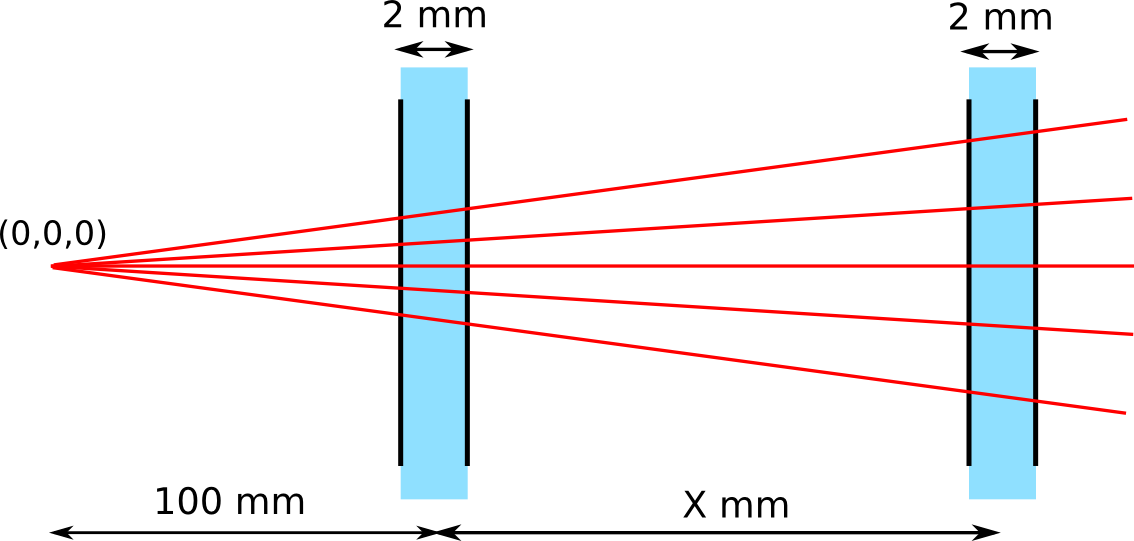
\includegraphics[scale=1.0]{./figures/rect3030.png}
%      \caption{G\'eom\'etrie du t\'elescope. Vue de cot\'e : dans le plan $yOz$. L'\'echelle PLUME 1 est d\'efinie comme celle croisant le faisceau en premier et l'\'echelle PLUME 2 est celle qui croise le faisceau en second.}
%     \label{fig:telescope_PLUMEs}
%     \end{center}
%    \end{figure}
% 
% \subsubsection{R\'esidus et distance inter-\'echelles}
%   
%   La largeur de la distribution des r\'esidus sur chacune des deux faces de l'\'echelle PLUME 2 a \'et\'e mesur\'ee en fonction de la distance inter-\'echelle $X$. Les r\'esultats obtenus sont visibles sur la figure \ref{fig:res_vs_dist}. La distance inter-\'echelle a \'et\'e fix\'ee aux valeurs de 5, 10, 20 et 40 $mm$. Les angles maximum d'ouverture du c\^one correspondant valent respectivement : 5.44, 5.19, 4.76 et 4.09 degr\'es. Les r\'esidus sont mesur\'es sur chacune des deux faces de l'\'echelle selon les directions $U$ et $V$ de l'\'echelle. Ainsi 16 points de mesure (rouge et noir) sont pr\'esents sur la figure \ref{fig:res_vs_dist}. De plus, des estimations th\'eoriques bas\'ees sur l'\'equation \ref{eq:propag_erreurs} sont indiqu\'ees en vert. Pour cette estimation on consid\`ere la r\'esolution constante (angle maximum 5.5 degr\'es).
%   
%   \medskip
%   Les distances des r\'esidus suivantes sont donn\'ees pour des échelles align\'ees parfaitement (valeurs Monte-Carlo). Pour une distance inter-\'echelle de $X = 5\, mm$, la largeur de la distribution des r\'esidus vaut respectivement 11 et 15.5 $\mu m$ sur la premi\`ere et la seconde face de l'\'echelle. Pour $X = 10 \, mm$, les r\'esidus sur la premi\`ere et la seconde face valent 22.5 et 27.5 $\mu m$. Pour $X = 20 \, mm$ on obtient respectivement 46 et 51.5 $\mu m$. Et, pour $X = 40 \, mm$, la valeur de la largeur de la distribution des r\'esidus vaut respectivement 95.5 et 100 $\mu m$ pour la premi\`ere et la seconde face.
%   
%   \medskip
%   
%   Les largeurs obtenues sont compar\'ees avec celles obtenues par un mod\`ele th\'eorique simple. Ce mod\`ele calcul simplement l'erreur attendue sur chaque face de l'\'echelle PLUME 2 en fonction de l'erreur sur les deux faces de l'\'echelle PLUME 1 \`a partir de la relation \ref{eq:propag_erreurs}. Le mod\`ele prend en compte uniquement des traces droites \`a incidence normale. \'Etant donn\'e la faible variation de la r\'esolution spatiale pour des angles d'incidence inf\'erieurs \`a 5 degr\'es on peut approximer la r\'esolution spatiale pour cette gamme d'inclinaisons \`a celle de la r\'esolution \`a incidence normale. C'est ce que nous avons fait. Comme notre mod\`ele s'ajuste parfaitement aux donn\'ees, notre hypoth\`ese est v\'erifi\'ee. De plus cela signifie que l'impact de la diffusion multiple est n\'egligeable. On notera toutefois qu'avec notre configuration, la diffusion multiple n'est plus n\'egligeable pour de grandes distances $X$. D'autres simulations ont montr\'ees que la diffusion multiple commence \`a jouer un r\^ole $\sigma_{ms} > 0.1 \, \mu m$ \`a partir d'environ $X = 300 \, mm$. Cette distance est toutefois bien plus grande que les distances utilis\'ees couramment \`a l'\'echelle d'un t\'elescope en faisceau.
%   
%   \begin{figure}[!Htb]
%     \begin{center} 
%      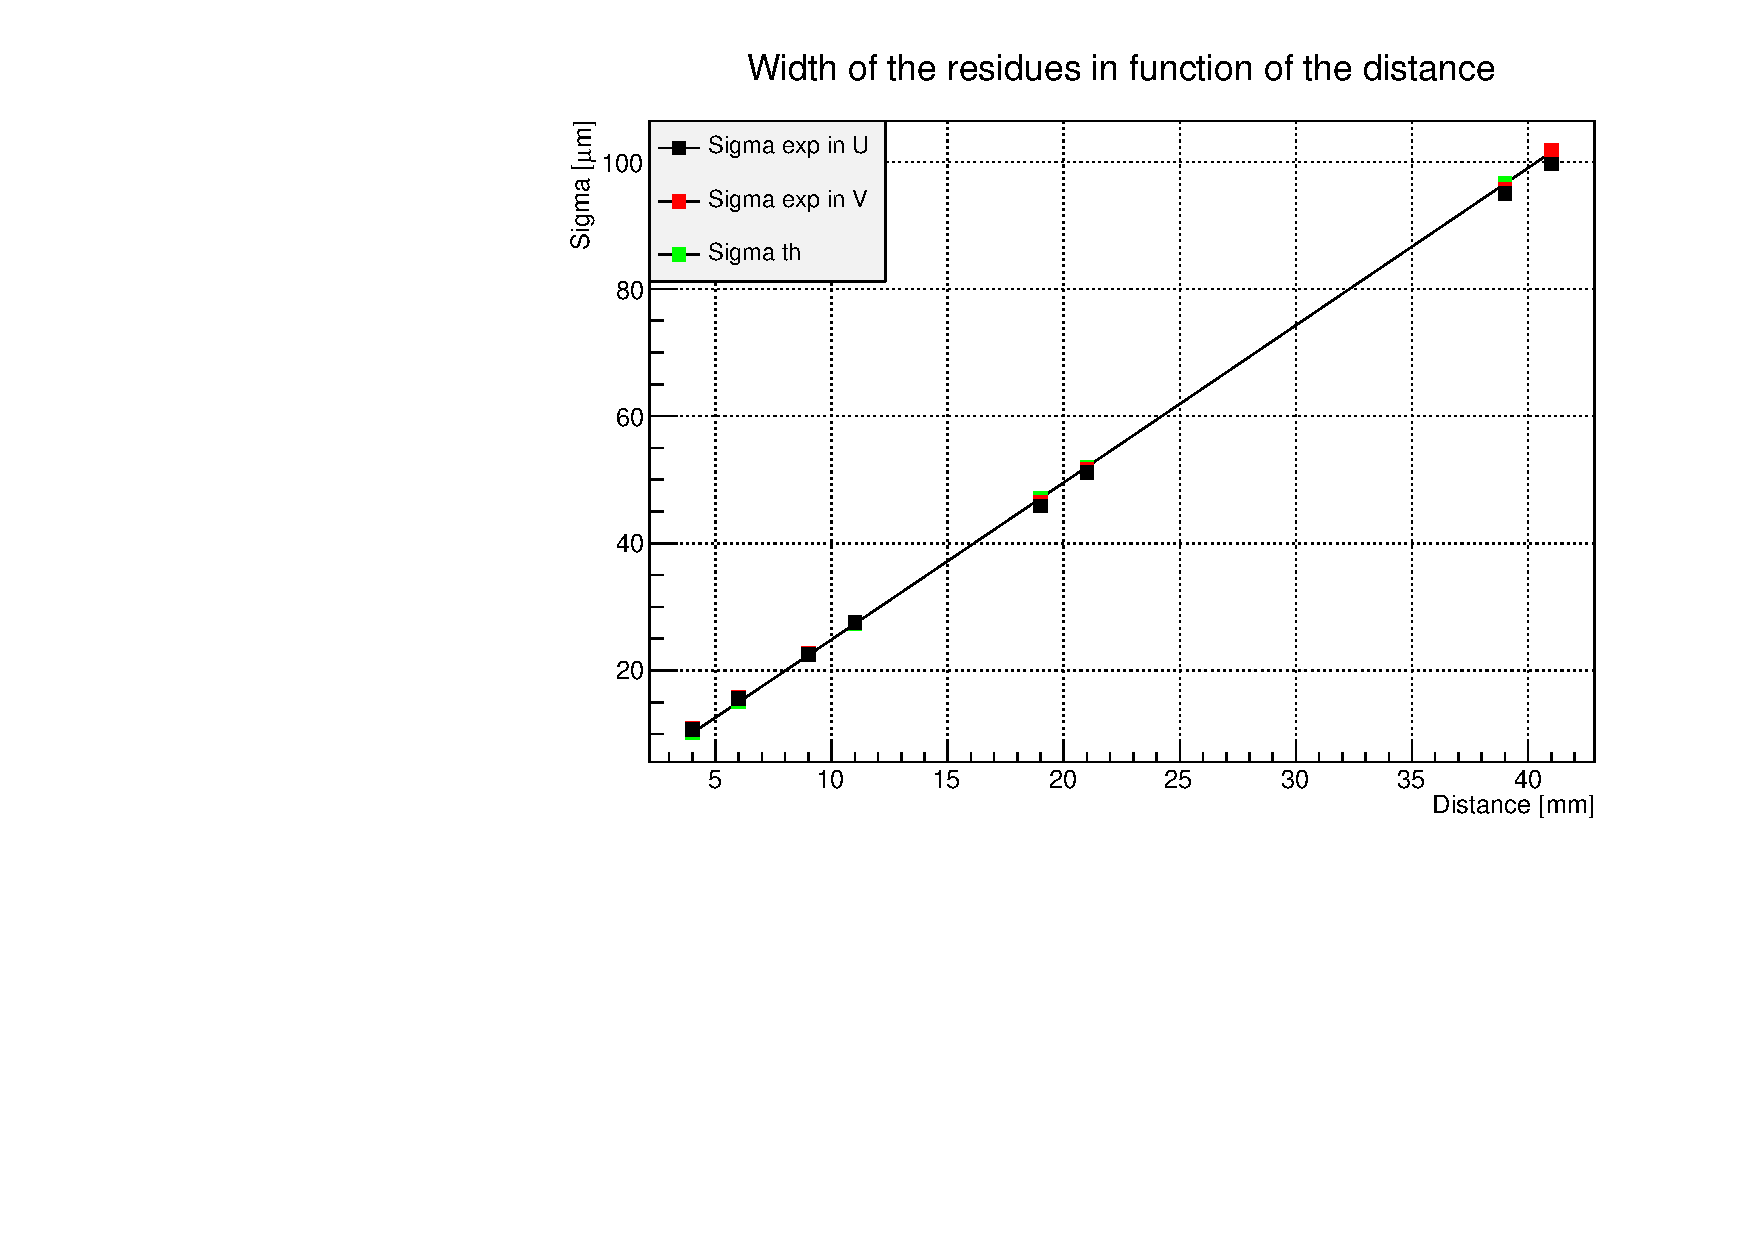
\includegraphics[scale=0.80]{./figures/Plots_analyses_simu/sigma_res_vs_distance.pdf}
%      \caption{Largeur de la distribution des r\'esidus en fonction de la distance entre les deux \'echelles PLUME. En noir la largeur de la distribution des r\'esidus selon l'axe U de l'\'echelle et en rouge selon l'axe V de l'\'echelle. En vert se trouve les pr\'evisions th\'eoriques.}
%     \label{fig:res_vs_dist}
%     \end{center}
%   \end{figure}
%   
%   \subsubsection{R\'esidus et impulsion du faisceau de pions}
%   
%   Pour cette \'etude nous utilisons la m\^eme configuration que pr\'ec\'edemment avec une distance $X = 5 \, mm$ fix\'ee. Nous allons cette fois-ci \'evaluer l'impact de la diffusion multiple en fonction de l'impulsion des pions. L'objectif \'etant d'\'evaluer jusqu'\`a quelle impulsion la diffusion multiple est n\'egligeable. Cette \'etude nous sera utile lorsque nous discuterons l'alignement de deux \'echelles, plac\'ees côte \`a c\^ote, \`a partir de leur zone de recouvrement. En effet, nous verrons dans le chapitre 6, traitant de l'alignement des \'echelles avec des mini-vecteurs, que nous ne consid\'ererons que des traces droites pour l'alignement.
%   
%   \medskip
%   
%   La figure \ref{fig:res_vs_imp} repr\'esente la largeur de la distribution des r\'esidus sur chacune des deux faces de l'\'echelle PLUME 2 en fonction de l'impulsion du faisceau de pions n\'egatifs. Cette figure montre que quelque soit l'axe U ou V de l'\'echelle, la largeur de la distribution des r\'esidus pour chaque face est la m\^eme. Ceci n'est pas \'etonnant puisque nous utilisons des pixels carr\'es et puisque l'inclinaison des traces utilis\'ees est faible. Cette inclinaison varie entre 0 et 5.5 degr\'es maximum selon les axes $Ox$ et $Oy$. Entre 1 $Gev$ et 120 $GeV$, sur chacune des faces de l'\'echelle 2, les r\'esidus ont sensiblement la m\^eme largeur. La diffusion multiple est alors n\'egligeable et nous retrouvons les valeurs pr\'ec\'edemment rencontr\'ees sur la figure \ref{fig:res_vs_dist} lorsque la distance inter-échelle \'etait de $X = 5 \, mm$, soit respectivement 11 et 15.5 $\mu m$ pour la premi\`ere et la seconde face de l'\'echelle PLUME 2. Cependant, pour des valeurs d'impulsions inf\'erieures \`a 1 $GeV/c$, la diffusion multiple joue un r\^ole non n\'egligeable et la largeur de la distribution des r\'esidus augmente en fonction de la diminution de l'impulsion du faisceau de pions n\'egatifs. Ainsi, pour la face 1 de l'\'echelle PLUME 2 la largeur de la distribution des r\'esidus passe de 11 $\mu m$ \`a 1 $GeV$ \`a 32 $\mu m$ \`a 25 $MeV$. Pour la face 2, cette largeur passe de 16 $\mu m$ \`a 1 $GeV$ \`a 54 $\mu m$ \`a 25 $MeV$.
%   
%   \medskip
% 
%   Pour conclure, avec une distance inter-\'echelle de 5 $mm$ et de faibles inclinaisons de traces, la diffusion multiple commence \`a jouer un r\^ole pour des valeurs d'impulsion du faisceau de pions inf\'erieures \`a 1 $GeV$. Autrement dit, pour des traces d'impulsions sup\'erieures \`a 1 GeV, celles-ci peuvent \^etre consid\'er\'ees droites, et nous pourrons les utiliser avec notre m\'ethode d'alignement utilisant les mini-vecteurs (voir chapitre 6).
%   
%   \begin{figure}[!Htb]
%     \begin{center} 
%      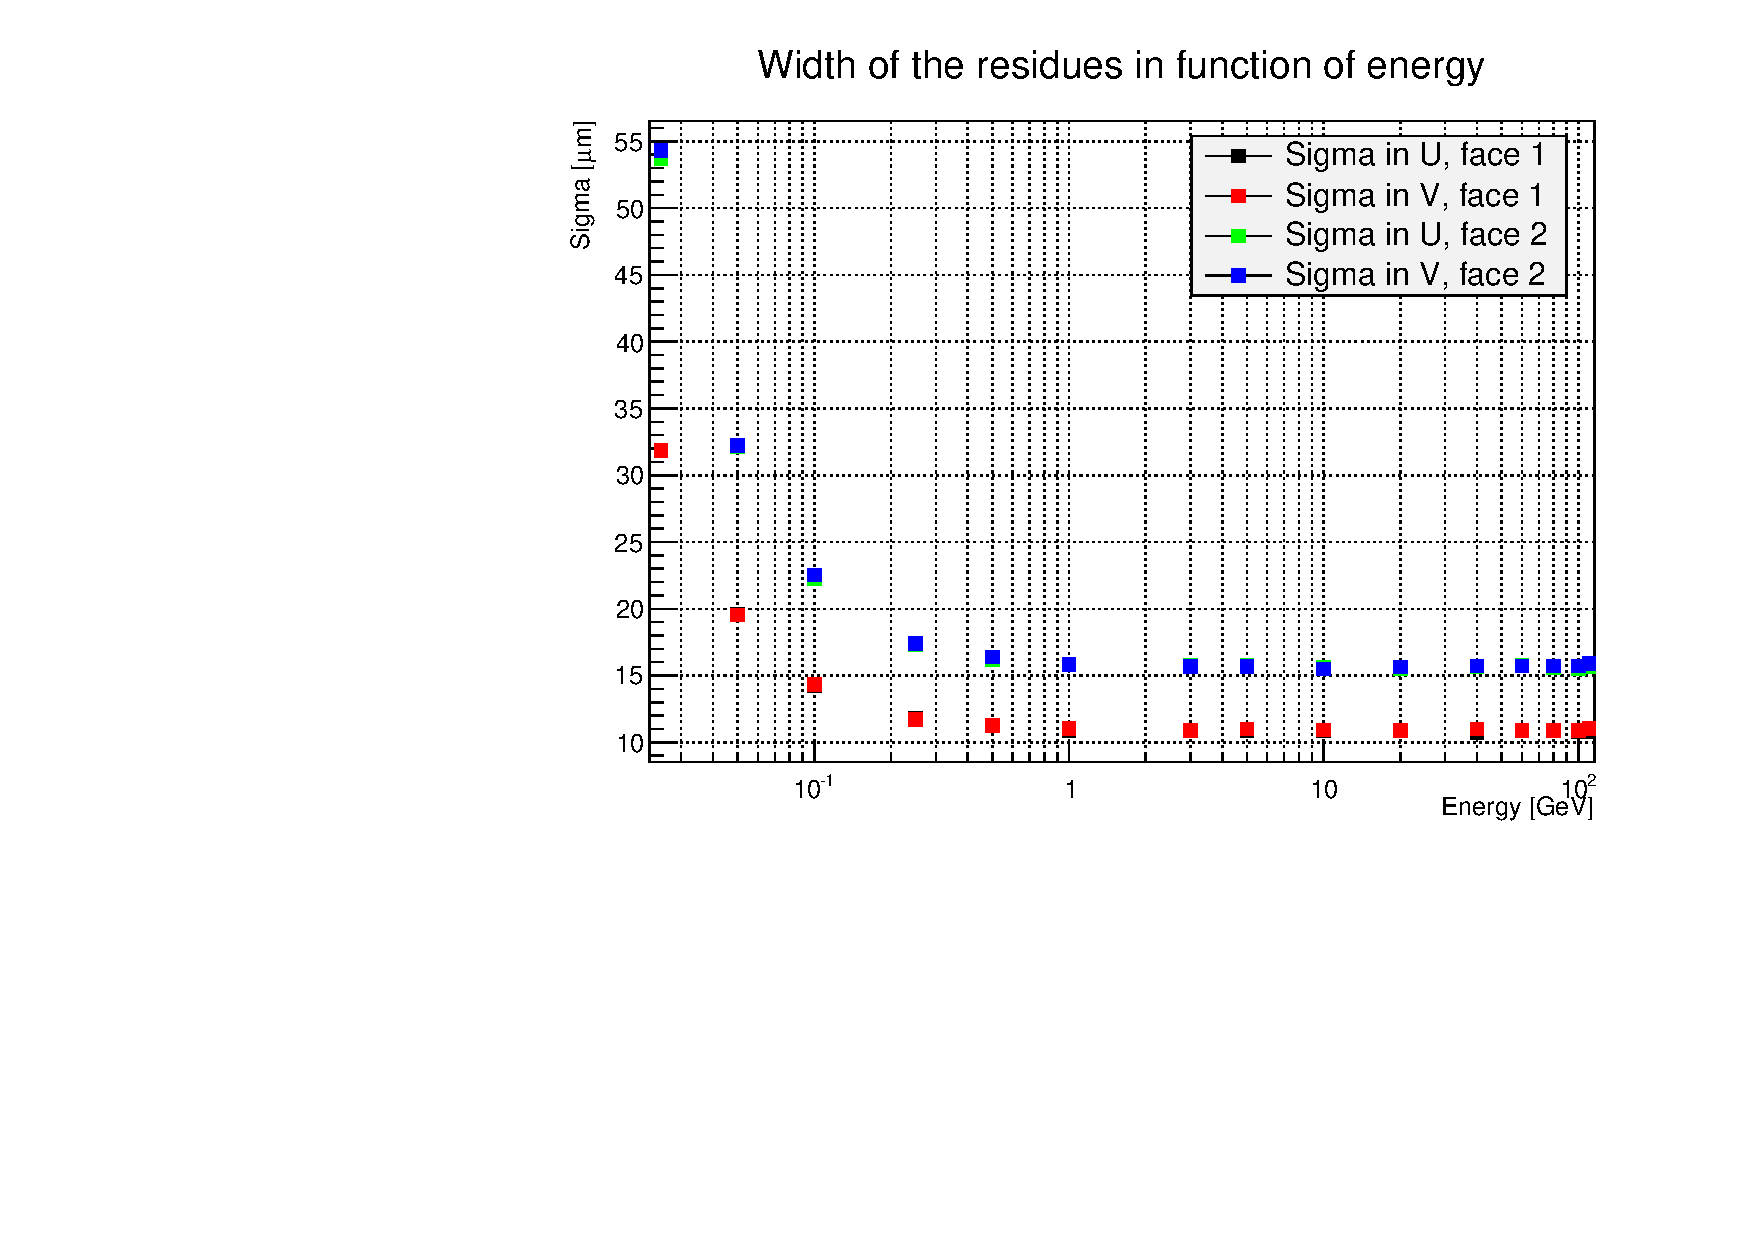
\includegraphics[scale=0.80]{./figures/Plots_analyses_simu/sigma_res_vs_E_echelle_log.pdf}
%      \caption{\'Evolution de la largeur de la distribution des r\'esidus en fonction de l'impulsion du faisceau de pions. L'\'echelle PLUME 1 est d\'efinie comme celle croisant le faisceau en premier et l'\'echelle PLUME 2 est celle qui croise le faisceau en second.}
%     \label{fig:res_vs_imp}
%     \end{center}
%   \end{figure}
% 
%   \FloatBarrier

 \section{Conclusion}

   Une simulation bas\'ee sur \textit{GEANT4} a permis de reproduire les donn\'ees des tests en faisceau du capteur MIMOSA-28 HR15. Les diff\'erences de performances entre simulation et donn\'ees sont inf\'erieures ou \'egale \`a $10 \%$. Ces r\'esultats on \'et\'e obtenus gr\^ace \`a un d\'epôt de charges de type \textit{Landau}, gr\^ace \`a un syst\`eme de r\'epartition des charges d\'epos\'ees dans les pixels du capteur bas\'e sur les donn\'ees des tests en faisceau, et gr\^ace \`a un syst\`eme de num\'erisation du signal. Diff\'erents objets comme les échelles PLUME ou encore les super-plans SALAT, ont pu \^etre \`a leur tour simul\'es \`a partir d'un assemblage de capteurs simul\'es. Les capteurs simul\'es ont alors \'et\'e caract\'eris\'es en fonction de l'angle d'incidence des traces. Les diff\'erents objets multi-capteurs d\'ecrits dans ce chapitre vont permettre la mise en place de m\'ethodes d'alignement adapt\'ees \`a leur g\'eom\'etrie. En particulier, la conception d'une m\'ethode d'alignement utilisant les mini-vecteurs sur la zone de recouvrement entre deux \'echelles PLUME cons\'ecutives va pouvoir \^etre mise au point et test\'ee.  

% De plus, les largeurs des r\'esidus avec un syst\`eme de deux \'echelles PLUME ont \'et\'e \'etudi\'ees en fonction de la distance entre les \'echelles et en fonction de l'impulsion du faisceau de pions \`a distance fix\'ee.
   
% Des estimations de certains param\`etres inconnus lors des tests en faisceau de MIMOSA-34, comme la diffusion multiple avec un faisceau d'\'electrons dot\'e d'une impulsion de $4.4 \, GeV/c$, ont ainsi pu \^etre \'etablies gr\^ace à nos simulations.

   %\bigskip

 %Dans notre cas des faisceaux de pions charg\'es n\'egativement sont envoy\'es sur un ensemble de capteurs CMOS. GEANT4 simule alors le d\'epot de charge a travers la couche épitaxiée de chaque capteur et modifie les trajectoires des particules en fonction du type de matiere travers\'e. Les capteurs utilis\'es sont organis\'es selon une g\'eom\'etrie bien d\'efinie. Cette g\'eom\'etrie sera d\'ecrite plus loin.

%\medskip

%Une contrainte majeure a orient\'e le choix de la modelisation des capteurs. En effet, le profil de dopage du silicium composant les capteurs n'est pas connu. Le fabricant le gardant secret. Il a alors fallu abandonner l'id\'ee de simul\'e le transport de chaque charge \`a travers la couche épitaxiée du capteur consid\'er\'e. Pour chaque capteur, un model bas\'e sur les donn\'ees des tests en faisceau a permis une \'evaluation statistique du transport de ces charges. Ainsi, on peut reconstruire la probabilit\'e pour un \'el\'ectron de finir son parcours absorb\'e par l'une des diodes.
